%!TEX encoding = UTF-8 Unicode

%% Projeto em Engenharia Aeroespacial 2023/24
%% Template para relattórios preliminar e final 
%%
%% Based on the example.tex file provided by Tomás Oliveira e Silva
%%
%% Modified by João Paulo Barraca <jpbarraca@ua.pt>
%% Modified by Filipe Manco <filipe.manco@ua.pt>
%% Modified by Pedro Casau <pcasau@ua.pt>

% Add 'final' parameter to remove "Relatório Intermédio" from cover page
\documentclass[11pt,twoside,a4paper]{report}

\usepackage[engineering,deti]{uaThesisTemplate}

%% Optional packages for utf8 encoding and T1 fonts
\usepackage[utf8]{inputenc}
\usepackage[T1]{fontenc}

%% For prettier pages
\usepackage{lmodern}

%% We will use english and portuguese
\usepackage[english,portuguese]{babel}

\usepackage{xspace}% used by \sigla

\usepackage[numbers,sort&compress]{natbib}
\usepackage{enumitem}
\usepackage{amsmath}
\usepackage{booktabs}
\usepackage{graphicx}
\usepackage{subcaption}
\usepackage{cleveref}
\usepackage{array}
\usepackage{mhchem}

%%%%%%%%%%%%%%%%%%%%%%%%%%%%%%%%%%%%%%%%%%%%%%%%%%
%%       DEFINE COVER FIELDS
%%                  START
%%%%%%%%%%%%%%%%%%%%%%%%%%%%%%%%%%%%%%%%%%%%%%%%%%


%%% Edit author's name
%% Author's full name
\Author{ALEXANDRE DE BRITO SALVADOR CAUVEL}

%%% Edit title in Portuguese
\TitlePT{Proteção contra a corrosão de ligas de alumínio com geometrias complexas através de conversion coatings}

%%% OPTIONAL: you can write your title in
%%%  other languages. You can repeat the following
%%%  line as many times as you want, or remove it
%%%  if you only want the portuguese title.
%% Optional Titles in additional languages.
\TitleEN{Corrosion protection of complex shapes aluminium alloys via conversion coatings}

%%% OPTIONAL: edit grant support texts where
%%%  appropriate. Maximum two.
%%%
%%% \GrantText{grant1}{grant2}
%% Optional Grant support texts
%\GrantText{Texto Apoio financeiro do POCTI no âmbito do III Quadro Comunitário de Apoio.}
%          {Texto Apoio financeiro da FCT e do FSE no âmbito do III Quadro Comunitário de Apoio.}

%%% OPTIONAL: Add a dedication text.
%% Optional Dedication text
%\Dedication{Dedico este trabalho à minha esposa e filho pelo incansável apoio.}

%%% OPTIONAL: Add an acknowledgement text
%% Optional Acknowledgement text
%%% OPTIONAL: edit acknowledgement text
\Acknowledgements{I would like to express my sincere gratitude to all my colleagues who supported me throughout this semester and were always available to help. I also extend my thanks to Dr. Aleksey Lisenkov for his valuable assistance in the initial laboratory part. 

I am deeply grateful to my supervisory team for their guidance and for their constant willingness to adapt to my existing knowledge. A special word of thanks goes to Dr. Kiryl Yasakau, who was always available to discuss every detail and provide support in both the laboratory and theoretical components, areas with which I was initially unfamiliar. His mentorship was fundamental to the completion of this work.}

%%% Edit the keywords and abstract in Portuguese
%%  Keywords and Abstract in Portuguese
%%% Keywords and Abstract in Portuguese
\Abstract{Palavras Chave}{Layered Double Hydroxides (LDH), Liga AC46000, Inibidores de Corrosão, Espetroscopia de Impedância Eletroquímica (EIS).}
         {Resumo}{\selectlanguage{portuguese}A indústria aeroespacial enfrenta a necessidade urgente de substituir os sistemas de proteção à corrosão à base de crómio hexavalente (Cr(VI)), de natureza carcinogénica, por alternativas ambientalmente sustentáveis que ofereçam níveis comparáveis de proteção ativa contra a corrosão. Os Layered Double Hydroxides (LDH) têm emergido como uma solução promissora, atuando como nanocontentores capazes de libertar inibidores de corrosão em resposta a estímulos ambientais, conferindo assim uma capacidade de “self-healing” ao sistema de revestimento. Este estudo centra-se na triagem preliminar de inibidores (WP2) para posterior intercalação em estruturas de ZnAl-LDH crescidas diretamente sobre a liga de alumínio fundido AC46000. Recorreu-se à Espectroscopia de Impedância Eletroquímica (EIS) para avaliar o desempenho do 2-mercaptobenzotiazol (MBT), do metavanadato de sódio (NaVO$_3$) e do molibdato de sódio (Na$_2$MoO$_4$) em solução de NaCl 0,05 M, ao longo de um período de imersão de 168 horas. Os resultados experimentais demonstram uma hierarquia clara na eficácia dos inibidores: o MBT apresentou o nível mais elevado de proteção, caracterizado por impedâncias significativamente mais altas a baixas frequências e por uma maior charge transfer resistance ao longo do tempo, seguido do NaVO$_3$. Em contraste, o Na$_2$MoO$_4$ revelou efeitos protetores negligenciáveis, com um desempenho semelhante ao do eletrólito não inibido. Estes resultados fornecem uma base científica sólida para a síntese e aplicabilidade subsequente de conversion coatings baseados em LDH a geometrias complexas típicas da indústria aeroespacial, com o objetivo de validar um sistema multicamada robusto e isento de crómio.}

%%% Keywords and Abstract in English
\Abstract{Keywords}{Layered Double Hydroxides (LDH), AC46000 Alloy, Corrosion Inhibitors, Electrochemical Impedance Spectroscopy (EIS).}
         {Abstract}{\selectlanguage{english}The aerospace industry faces a critical requirement to replace carcinogenic hexavalent chromium (Cr(VI)) protective systems with environmentally friendly alternatives that provide comparable active corrosion protection. Layered Double Hydroxides (LDH) have emerged as a promising solution, functioning as nanocontainers that release corrosion inhibitors in response to environmental triggers, thereby imparting a "self-healing" capability to the coating system. This study focuses on the preliminary screening of inhibitors (WP2) for subsequent intercalation into ZnAl-LDH structures directly grown on the AC46000 aluminium cast alloy. Using Electrochemical Impedance Spectroscopy (EIS), the performance of 2-mercaptobenzothiazole (MBT), sodium metavanadate (NaVO$_3$), and sodium molybdate (Na$_2$MoO$_4$) was evaluated in 0.05 M NaCl over a 168-hour immersion period. Experimental results demonstrate a clear hierarchy in inhibitor efficiency: MBT provided the highest level of protection, characterized by significantly higher low-frequency impedance and charge-transfer resistance, followed by NaVO$_3$. In contrast, Na$_2$MoO$_4$ displayed negligible protective effects, performing similarly to the uninhibited electrolyte. These findings provide a scientific basis for the subsequent synthesis and functionalization of LDH conversion layers on complex aerospace geometries, aiming to validate a robust, chromium-free multilayer protective system.}


%%%%%%%%%%%%%%%%%%%%%%%%%%%%%%%%%%%%%%%%%%%%%%%%%%
%%       DEFINE COVER FIELDS
%%                  END
%%%%%%%%%%%%%%%%%%%%%%%%%%%%%%%%%%%%%%%%%%%%%%%%%%

\begin{document}

%%% By default we consider portuguese to be the
%%%  main language (the last one in the usepackage
%%%  declaration). If you're writing your document
%%%  in english uncomment the following line.
%%% Set the proper language or you will end with incorrect hyphenation!
\selectlanguage{english}

\MakeCover

% Disable addition of ToC, LoF and LoT to the table of contents
\addtocontents{toc}{\protect\setcounter{tocdepth}{-1}}

\tableofcontents

\listoffigures
\listoftables

\newpage

% Restore the default value (chapter-level)
\addtocontents{toc}{\protect\setcounter{tocdepth}{2}}

\chapter{Introduction}
\section{Background}
Modern aerospace structures rely heavily on high-performance aluminium alloys, especially the 2xxx and 7xxx series, due to their exceptional strength-to-weight ratio and ease of manufacturability. However, under the harsh conditions of the aerospace environment, these materials are highly susceptible to localized corrosion \cite{MartinezViademonte2020,Garg2025}. This degradation is accelerated by intermetallic particles dispersed within the alloy that form micro-galvanic sites, which can significantly shorten a component's lifespan \cite{MartinezViademonte2020,Becker2019,Garg2025}.

Traditionally, this challenge has been managed using multilayer coatings based on hexavalent chromium (Cr(VI)) \cite{MartinezViademonte2020,BoualiReview2020}. These coatings offered strong adhesion, long-term durability, and, most importantly, a self-healing capability \cite{MartinezViademonte2020,Becker2019,BoualiReview2020}. However, due to the carcinogenic nature of Cr(VI), strict regulatory restrictions have demanded an immediate ban, creating a need for safe, high-performance alternatives that can match the protection offered by chromium-based systems \cite{MartinezViademonte2020,Becker2019,Bouali2020}.

Recently, Layered Double Hydroxides (LDH) have emerged as a particularly promising alternative \cite{Cao2022,Becker2019,Bouali2020,Zhou2017,Iuzviuk2020,BoualiReview2020}. Their layered structure allows them to store and release corrosion inhibitors in response to changes in the environment, providing a combination of barrier protection and active self-healing that aligns well with the industry's long-term needs.

Much of the recent research on LDH coatings has focused on common wrought alloys such as AA2024, usually tested on simple flat samples \cite{Tedim2014,Tedim2011,He2020,Bouali2020}. While these studies have demonstrated excellent potential, there is a distinct lack of data on how LDH coatings perform on cast alloys like AC46000. Cast alloys make it possible to manufacture complex, highly detailed geometries that are becoming more common in modern aerospace assemblies. But these components also introduce new challenges such as an uneven surface roughness, restricted accessibility, distinct microstructural features, and higher silicon content. All of these factors can significantly influence LDH growth, inhibitor incorporation, and overall coating uniformity, integrity and performance.

By successfully applying and testing the optimized environmentally-friendly LDH system on geometrically complex components, this work validates the limited existing research. More importantly, it draws a path for future work, especially in complex geometry which continues to grow rapidly in aerospace industry, while complying with safety and health regulations.

\section{Objectives}
This work follows four central objectives defined in the project plan:
\begin{itemize}
    \item \textbf{O1. Synthesis and Optimization:} Synthesize a, Layered Double Hydroxide (LDH) conversion pre-treatment capable of forming a uniform coating layer on both flat and geometrically complex aluminium alloy substrates.
    
    \item \textbf{O2. Inhibitor Integration:} Intercalate established and novel corrosion inhibitors into the optimized LDH structure.
    
    \item \textbf{O3. Performance Benchmarking:} Compare LDH performance against established reference systems, such as anodizing and Cr(III)/Ce(IV) conversion coatings.
    
    \item \textbf{O4. Applicability to complex shapes:} Validate the protective system on complex geometric shapes, including application of an organic top-coating.
\end{itemize}

\section{Scope}
\begin{itemize}
    \item \textbf{Coating System:} Hydrothermal synthesis and optimization of ZnAl-LDH conversion layers on AC46000 alloy via immersion in a metal-containing solution at high temperatures.
    
    \item \textbf{Inhibitor chemistry:} A targeted screening of environmentally friendly candidates, including vanadates, molybdates and MBT, will be performed at a standard concentration of 0.005 M.
    
    \item \textbf{Characterization Techniques:} Physical Characterization will use XRD to evaluate inhibition intercalation efficiency, FTIR/Raman to confirm chemical presence of inhibitor molecules within the LDH galleries, and SEM/EDS to analyse coating and substrate morphology.
    
    \item \textbf{Electrochemical Assessment:} Corrosion performance is evaluated through long-term EIS (up to 168 hours of immersion in 0.05 M NaCl) and localized SVET for self-healing monitoring.
    
    \item \textbf{Multilayer Configuration:} The final validation phase employs an anaphoretic polyurethane-based organic coating applied over the optimized LDH pre-treatment.
\end{itemize}

\section{Work Breakdown Structure (WBS)}
To achieve the defined objectives, the research project is organized into seven distinct Work Packages (WPs) that provide a chronological and technical framework for execution. This structure ensures a systematic progression from theoretical review and material characterization to the synthesis and final validation of the LDH-based protective system on complex geometries. Table \ref{tab:wbs_summary} summarizes the project phases, their respective timelines, and the key deliverables associated with each stage of the research.

\begin{table}[htbp]
    \centering
    \small
    \renewcommand{\arraystretch}{1.5} % Increases the vertical gap between rows
    \caption{Work Breakdown Structure (WBS) summary and project timeline.}
    \label{tab:wbs_summary}
    \begin{tabular}{lll>{\raggedright\arraybackslash}p{5cm}}
        \toprule
        WP & Title & Timeline & Key Tasks \& Deliverables \\
        \midrule
        1 & State-of-the-Art & Sep -- Oct 25 & Literature review on Al corrosion and LDH systems. \\
        2 & Inhibitor Selection & Oct -- Dec 25 & EIS screening of organic/inorganic inhibitors in NaCl. \\
        3 & Substrate Charact. & Nov -- Jan 26 & Preparation and characterization of AC46000 substrate. \\
        4 & LDH Synthesis & Dec -- Feb 26 & Growth of LDH on Al and intercalation of inhibitors (XRD/FTIR). \\
        5 & Corrosion Eval. & Mar -- May 26 & EIS/SVET benchmarking against reference systems. \\
        6 & Multilayer Coatings & May -- Jun 26 & Organic coating on complex parts and adhesion validation. \\
        7 & Final Report & Jan -- Jun 26 & Data compilation and feasibility assessment. \\
        \bottomrule
    \end{tabular}
\end{table}


\chapter{Literature Review}
\section{Thermodynamic basis for corrosion}

Corrosion is fundamentally a spontaneous thermodynamic process driven by the tendency of metals to revert to their most stable, lower-energy states, such as oxides ($M_nO_p$) or sulfides ($M_nS_p$) \cite{Sastri2007,Revie2008,Vargel2020}. This transition is quantified by a negative change in Gibbs free energy ($\Delta G$), indicating that the oxidation reaction is energetically favored over the metallic state. Mathematically, this thermodynamic drive is linked to the electrochemical potential, $E$, through the relation:
\begin{equation}
\Delta G = -n F E
\label{gibs}
\end{equation}

where $n$ is the number of electrons transferred and $F$ is the Faraday constant \cite{Sastri2007,Ghali2010,Revie2008}.

\section{Charge Transfer and the Electric Double Layer (EDL)}
An electrochemical reaction can be described by the transfer of electrical charge (electrons) across the interface between an electrode (metal) and an electrolyte (aqueous, conductive solution) \cite{Vargel2020,Sastri2007,Revie2008,Ghali2010}.

This interface is characterized by the formation of the Electric Double Layer (EDL), a region where ions and water molecules rearrange into distinct planes (The compact stern/helmholtz layers and the diffuse Gouy-Chapman region) to maintain overall electrical neutrality \cite{Vargel2020,Ghali2010,Sastri2007}. The EDL plays a key role in corrosion because it acts as a selective barrier that ions must cross for electrochemical reactions to take place \cite{Vargel2020,Ghali2010,Marcus2011}. 

\section{Aluminium Corrosion}

For aluminium, the corrosion mechanism can be summarized in a simplified 
way by two coupled half-reactions. Firstly, the anodic oxidation \cite{Vargel2020,Ghali2010}:
\begin{equation}
\mathrm{Al} \rightarrow \mathrm{Al}^{3+} + 3e^-
\end{equation}
And to balance this, the released electrons must be consumed by a reduction 
reaction occurring in the surrounding environment, which is called the cathodic reduction:
\begin{equation}
2\mathrm{H}_2\mathrm{O} + \mathrm{O}_2 + 4e^- \rightarrow 4\mathrm{OH}^-
\end{equation}

Overall, aluminium corrosion can be represented by the global reaction \cite{Vargel2020,Ghali2010}:
\begin{equation}
\mathrm{Al} + 3\mathrm{H}_2\mathrm{O} \rightarrow \mathrm{Al(OH)}_3 + \frac{3}{2} \mathrm{H}_2
\end{equation}
In this process, aluminium is oxidized forming aluminium hydroxide, 
$\mathrm{Al(OH)}_3$, a hydrated form of alumina.

\section{Notion of Potential and Passivity}
\label{potential}
Up to this point, the discussion has addressed aluminium's thermodynamic tendency to revert to a stable oxidized state. In real environments, this behaviour is governed by electrochemical potentials that describe the metal's response in solution.

At the metal-electrolyte interface, charge separation across the metal surface, Helmholtz layers, and diffuse layer gives rise to an electrode potential \cite{Vargel2020,Sastri2007,Ghali2010}. While standard electrode potentials provide useful thermodynamic insight, they are determined under idealized conditions and have limited practical relevance. Consequently, corrosion studies typically rely on the open-circuit potential (OCP), defined as the potential difference between a metal and a reference electrode at equilibrium and in the absence of an external current \cite{Vargel2020,Roberge2000}. Because absolute potentials cannot be measured, OCP values are always reported relative to a reference electrode in a given electrolyte \cite{Vargel2020,Sastri2007,Revie2008}.

The open circuit potential (OCP) should be distinguished from the standard electrode potential ($E^\circ$), usually used in Eq.~\ref{gibs}, which represents the ideal thermodynamic driving force for a given half-reaction. For aluminium, $E^\circ = -1.66\ \mathrm{V}$ versus the standard hydrogen electrode (SHE), which serves as the 0V reference. In contrast, the OCP reflects the steady-state potential established in a specific environment, where anodic and cathodic reactions are balanced \cite{Sastri2007,Revie2008,Marcus2011}. In aqueous environments, aluminium typically exhibits an OCP around $-0.5\ \mathrm{V}$ versus SHE \cite{Vargel2020,Revie2008}. This apparent discrepancy arises from the rapid formation of a thin, adherent alumina film upon exposure to air, which modifies the metal--electrolyte interface.

\begin{equation}
2\mathrm{Al} + \frac{3}{2} \mathrm{O}_2 \rightarrow \mathrm{Al}_2\mathrm{O}_3
\end{equation}
This passive oxide layer significantly slows further oxidation, although its stability depends on environmental factors such as pH, temperature, and the presence of aggressive ions, particularly chlorides \cite{Vargel2020,Sastri2007,Ghali2010,Revie2008}.

While pure aluminium provides a useful reference, practical applications involve aluminium alloys, whose corrosion behaviour is strongly influenced by microstructural inhomogeneities, especially intermetallic phases (IMPs) \cite{Vargel2020,Ikeuba2024,Marcus2011,Sastri2007}. 

\section{IMPs as Corrosion Drivers}

Intermetallic phases (IMPs) are compounds formed by two or more metallic elements that occur within alloy microstructures with a stoichiometry different from that of the parent alloy \cite{Vargel2020,Ikeuba2024}. Depending on their composition, IMPs can be classified as anodic or cathodic relative to the aluminium matrix, based on whether their open-circuit potential (OCP) is lower or higher than that of the matrix \cite{Vargel2020,Ikeuba2024,Marcus2011}.

Differences in electrochemical potential between IMPs and the surrounding matrix drive galvanic corrosion, as electrons flow from anodic sites to cathodic ones. The resulting corrosion morphology depends strongly on the spatial distribution of IMPs: dispersed particles tend to promote pitting corrosion, whereas IMPs concentrated along grain boundaries can lead to intergranular corrosion \cite{Vargel2020,Ghali2010,Marcus2011,Sastri2007}.

Anodic IMPs preferentially dissolve or dealloy, leaving cavities within the aluminium matrix. In contrast, cathodic IMPs remain intact and accelerate dissolution of the surrounding matrix, producing a characteristic ring-shaped corrosion pattern \cite{Vargel2020,Ikeuba2024,Marcus2011}. Cathodic IMPs are considered more detrimental because they continuously sustain corrosion processes. At these sites, oxygen reduction generates hydroxide ions, increasing the local pH and further destabilizing the aluminium matrix \cite{Marcus2011,Vargel2020,Ikeuba2024}. Given the amphoteric nature of aluminium, elevated pH conditions significantly enhance its corrosion rate \cite{Vargel2020}.

In some cases, initially anodic particles may undergo partial dissolution, leaving behind a highly cathodic remnant. This process, known as dealloying or polarity reversal, results in localized corrosion behaviour similar to that induced by cathodic IMPs \cite{Vargel2020,Ikeuba2024,Marcus2011}.

The presence of aggressive species such as chloride ions further exacerbates corrosion. Due to imperfections in the native oxide film, chloride ions can penetrate the alumina layer and replace oxygen atoms within its structure, compromising its integrity and promoting local breakdown \cite{Vargel2020,Ikeuba2024}. Once the oxide film is breached, chlorides can directly interact with aluminium according to:
\begin{equation}
\mathrm{Al} + n\mathrm{Cl}^- \rightarrow \mathrm{AlCl}_n + 3e^-
\end{equation}
Since corrosion is an irreversible process, mitigation strategies focus on preventing or retarding these mechanisms through the use of protective systems.

\section{Conventional Corrosion Protection Methods}

Conventional corrosion protection systems for aluminium alloys, particularly in aerospace applications, typically consist of a multilayer structure comprising an anodic oxide or conversion coating, followed by a corrosion-inhibited primer and an organic topcoat \cite{MartinezViademonte2020}. These systems are designed to provide both passive barrier protection and active corrosion inhibition.

Although anodized aluminium alloys generally exhibit superior corrosion and wear resistance, conversion coatings (CCs) are often preferred due to their lower cost, simpler processing, and faster application. CCs can be applied by immersion, spraying, or wipe techniques, making them well suited for industrial use \cite{Becker2019}. In such systems, passive protection is provided by the coating layers, while active protection is achieved through corrosion inhibitors that become effective when coating defects allow electrolyte ingress \cite{MartinezViademonte2020}.

Historically, hexavalent chromium has played a central role in these systems, both as chromate conversion coatings and as a leachable inhibitor due to its self-healing capability \cite{Beneke2016,BoualiReview2020}. However, Cr(VI) compounds are highly toxic and carcinogenic, leading to severe regulatory restrictions and the need for environmentally benign alternatives \cite{MartinezViademonte2020,BoualiReview2020}.

Among the proposed replacements, trivalent chromium process (TCP) coatings have gained industrial acceptance due to their good corrosion protection performance on aluminium alloys \cite{Becker2019,Qi2015,BoualiReview2020}. Nevertheless, TCP systems exhibit reduced effectiveness when combined with non-chromium primers, and trace formation of Cr(VI) during processing remains a concern. These limitations raise questions about TCP coatings as a universal solution and motivate the development of alternative strategies.

Rare earth conversion coatings (RECCs), particularly cerium-based systems, have also been investigated as chromate alternatives due to their lower toxicity and reported corrosion protection performance comparable to CCCs \cite{Becker2019,Hughes2009,Cohen1995,Lau2009}. However, their lack of strong self-healing behaviour and sensitivity to environmental conditions and substrate chemistry limit their reliability and widespread industrial adoption.

\section{Layered Double Hydroxide (LDH) as an alternative}
More recently, layered double hydroxides (LDH) have emerged as a promising alternative material. LDH are a class of lamellar materials belonging to brucite-like structures. These compounds consist of positively charged host layers and exchangeable anions located in the interlayer galleries to maintain charge balance \cite{Bouali2020,Zhou2017,He2020,Iuzviuk2020,Cao2022}. Generally, the chemical structure of LDH can be represented by the general formula:

\begin{equation}
[\mathrm{M}^{2+}_{1-x}\mathrm{M}^{3+}_{x}(\mathrm{OH})_{2}]^{x+}(\mathrm{A}^{n-})_{x/n} \cdot m\mathrm{H}_{2}\mathrm{O}
\label{eq1}
\end{equation}

where $\text{M}^{2+}$ and $\text{M}^{3+}$ represent the divalent and trivalent metallic cations, respectively, which form the brucite-like layers with $\text{OH}^{-}$. $\text{A}^{n-}$ corresponds to the $n$-valent anionic species located at the hydrated interlayer galleries to balance the charge, $x$ represents the molar ratio $\text{M}^{3+}/(\text{M}^{2+} + \text{M}^{3+})$, typically ranging between 0.2 and 0.33, and $m$ represents the number of moles of water 
molecules between the layers\cite{He2020,Cao2022}.

The cations $\text{M}^{2+}$ and $\text{M}^{3+}$ in the host layer can be replaced with other cations to form LDH as long as the radius of the cations is appropriate \cite{He2020}. The interaction between the hydroxide layers and the interlayer anions is relatively weak, relying mainly on electrostatic forces and hydrogen bonding \cite{He2020}. As a result, the interlayer anions can be readily exchanged with other anionic species. 

Because of the controllable composition of cations or interlayer anions, LDH have been widely investigated for applications such as adsorption, catalysis, drug delivery, flame retardancy, and, more recently, corrosion protection \cite{He2020}. Following the pioneering work of \citet{Buchheit2003}, numerous studies have demonstrated enhanced corrosion resistance when LDH are applied to aluminium, zinc, and magnesium alloys, as well as to anodized surfaces and galvanized steels \cite{Iuzviuk2020}.

\subsection{Advantages of LDH}

The ease of anion exchange is a key feature that makes LDH particularly attractive for corrosion protection. This property can be exploited in two complementary ways \cite{Iuzviuk2020,He2020,Cao2022,Zhou2017,Bouali2020}:
\begin{enumerate}
    \item Controlled release of corrosion inhibitors: LDH can act as hosts for anionic corrosion inhibitors within their interlayers, releasing them on demand in response to environmental triggers such as pH changes or the presence of aggressive species (i.e. $\text{Cl}^-$,$\text{SO}_4^{2-}$). This responsive behavior provides LDH-based systems with "self-healing" properties. When appropriate inhibitors are intercalated, these systems can achieve corrosion protection performance comparable to traditional Cr(VI)-based compounds.
    \item Trapping of corrosive species: Simultaneously, LDH can capture harmful anions in their interlayer galleries, effectively functioning as nanotraps while releasing inhibitors.
\end{enumerate}


Beyond these advantages, several additional features make LDH a particularly appealing alternative \cite{Cao2022}. In addition to the above-mentioned "self-healing" effect, LDH can undergo local dissolution and recrystallization, forming new crystals that fill defects and restore protection. Furthermore, when LDH are incorporated into coatings, this active behavior is complemented by a passive barrier contribution, as LDH particles fill micro- and nanopores and increase the tortuosity of diffusion pathways and hindering water permeation. This so-called labyrinth effect can be further enhanced by combining LDH with graphene.

LDH can also contribute through a physical barrier effect at the crystal level. As demonstrated by \citet{Bouali2020}, exchanging nitrate ions with smaller anions such as chlorides in ZnAl-LDH reduces the interlayer spacing, resulting in a denser structure that restricts species diffusion through the crystal lattice. Importantly, LDH-based systems can benefit from synergistic effects, in which the combined action of different inhibitors or protection mechanisms leads to performance beyond the sum of the individual contributions.

\subsection{Synthesis of LDH}

Layered double hydroxides (LDH) can be fabricated either ex situ as powders or in situ as films directly grown on metal substrates for corrosion protection. LDH powders are most commonly synthesized by co-precipitation, which can be carried out under variable pH (titration co-precipitation) or constant pH conditions. According to \citet{BoualiReview2020} constant pH synthesis is generally preferred, as it leads to purer and more crystalline LDH. In this process, the pH is maintained by the simultaneous addition of an alkaline solution (such as NaOH or NH$_{3}\cdot$H$_{2}$O) and a mixed-metal salt precursor solution containing the cations that form the LDH structure. The alkaline solution is selected based on the metal salts used and the anion intended for intercalation within the LDH galleries. 

The main advantage of LDH powders lies in their versatility. They can be dispersed within a single coating system, such as sol--gel hybrid coatings, as reported by \citet{Yasakau2014} and \citet{Alvarez2010}, or distributed across multilayer coating architectures, which is a common approach in industrial applications such as the automotive sector \cite{BoualiReview2020}.

Despite this flexibility, in situ LDH growth is generally considered more advantageous for corrosion protection. This method promotes the formation of chemical bonds between the LDH film and the substrate, resulting in stronger adhesion, as reported by \citet{BoualiReview2020,Cao2022} and \citet{Guo2009}. In addition, in situ film formation is a one-step process that is largely independent of substrate geometry, making it suitable for large-area applications \cite{Guo2009,BoualiReview2020}.

The simplest and most widely used in situ LDH growth method is hydrothermal treatment, as described by \citet{Guo2009}, or in situ co-precipitation, as referred to by \citet{BoualiReview2020}, which can be regarded as an extension of the co-precipitation approach described earlier. Some authors, including \citet{Cao2022} and \citet{Zhou2017}, consider the hydrothermal method to be more complex due to the requirement for an autoclave.

It should be noted that the distinction made by \citet{Cao2022} regarding weaker interfacial bonding applies specifically to the in situ co-precipitation route described in that work, where the metal cations are supplied predominantly from the solution rather than from the substrate. This limitation does not apply to the in situ co-precipitation approach described by \citet{BoualiReview2020}, in which the substrate contributes metal ions to the LDH structure, resulting in bonding characteristics more comparable to those obtained via hydrothermal treatment. For this reason, the reader is encouraged to focus on the process itself rather than on differences in terminology. 

In this work, the approach described by \citet{BoualiReview2020} will be adopted, in which the substrate serves as one of the metal precursors. For aluminium substrates, LDH films are typically fabricated by immersing the substrate in a solution containing divalent or monovalent metal cations (such as Zn$^{2+}$, Mg$^{2+}$, or Li$^{+}$) under controlled pH, temperature, and concentration conditions, while Al$^{3+}$ ions are supplied through partial dissolution of the substrate. This type of synthesis is widely adopted due to its simplicity and the strong interfacial bonding it produces between the LDH film and the substrate \cite{Cao2022, Guo2009}, and it has been employed in numerous corrosion protection studies such as \cite{Iuzviuk2020, Tedim2014,Tedim2011}.

In addition to this synthesis process, other in situ fabrication techniques have been explored. Electrodeposition offers significantly shorter processing times, with deposition times of approximately 300~s as reported by \citet{He2020}, and can be applied to substrates with complex geometries \cite{Cao2022}. However, it generally results in weaker film adhesion and higher energy consumption \cite{Cao2022}. Steam coating represents another promising alternative, combining good bonding strength with an environmentally friendly process \cite{Pan2023, Cao2022}. Although this technique was previously limited to magnesium alloys, \citet{Matsui2025} recently demonstrated its successful application to a die-cast aluminium alloy (ADC-12) for the formation of Mg-Al LDH films.

\subsection{Corrosion inhibitors}
LDH are typically synthesised with nitrate ions as the initial interlayer anions, as nitrates can be readily exchanged. In contrast, carbonate anions exhibit a much stronger affinity for LDH structures, which hinders subsequent anion exchange \cite{Cao2022}. Once the LDH has been produced, an anion-exchange step is performed to intercalate the desired corrosion inhibitor.

A wide range of corrosion inhibitors has been investigated for LDH-based systems. Vanadates are among the most extensively studied inhibitors. Active corrosion protection for AA2024 has been reported by \citet{Tedim2011} and \citet{Yasakau2014}, while \citet{Zhang2015} demonstrated that vanadate-intercalated ZnAl-LDH provides better corrosion resistance than nitrate-intercalated LDH for the same alloy. Similar protective behavior was also observed for AZ91 magnesium alloy by \citet{Zhou2017} using ZnAl-LDH. Other inhibitors, such as 2-mercaptobenzothiazole (MBT) and molybdates, have also been studied \cite{Cao2022,Tedim2010,Zhang2015}, but for AA2024 they were found to offer inferior corrosion protection compared to vanadates \cite{Zhang2015,Tedim2010}.

In contrast, \citet{Matsui2025} reported superior corrosion resistance for molybdate-intercalated Mg-Al LDH compared to vanadates when applied to ADC-12, an Al-Si-Cu casting alloy. This highlights that inhibitor performance can be strongly dependent on both the LDH composition and the substrate material.

Synergistic effects between different inhibitors have also been reported. \citet{Zhang2015} demonstrated enhanced corrosion protection when cerium salts were combined with vanadates, while \citet{Tedim2010} showed that LDH nanocontainers loaded with both vanadate and MBT anions provided a synergistic anticorrosion effect. Additionally, \citet{Lamaka2007} reported that organic inhibitors such as 8-hydroxyquinoline (8-HQ), salicylaldoxime, and quinaldic acid can suppress corrosion of AA2024 as effectively as, or in some cases more effectively than, MBT and cerium salts.

\subsection{Electrochemical techniques for inhibitor screening}
In LDH-based corrosion protection systems, electrochemical techniques are commonly used to evaluate inhibitor performance. Among these, electrochemical impedance spectroscopy (EIS) is widely applied due to its non-destructive nature and sensitivity to interfacial processes. EIS effectively assesses inhibitor efficiency and barrier properties in aluminium alloys, as impedance changes reflect inhibitor adsorption or release from LDH structures \cite{Alvarez2010,Zheludkevich2010,Zhou2017,Zhang2017,He2020,Lamaka2007,Tedim2011,Yasakau2014}. Consequently, it is often used to screen promising inhibitors before their incorporation into LDH-based systems.


\chapter{Methodology}
As established in the work plan for WP2, the preliminary phase involves the electrochemical screening of candidate inhibitors via EIS to select the most effective species for LDH integration.

\section{Electrochemical Impedance Spectroscopy (EIS)}

Electrochemical Impedance Spectroscopy (EIS) is an electrochemical technique commonly used to investigate corrosion processes and interfacial phenomena \cite{Joshua2025}. In EIS, a small sinusoidal voltage perturbation is applied to an electrochemical system over a range of frequencies, and the resulting current response is measured \cite{Joshua2025,Lazanas2023}. This approach enables the separation and analysis of electrochemical processes occurring at the electrode-electrolyte interface, including charge transfer and double-layer behaviour.

For this work, EIS measurements were performed using a standard three-electrode configuration consisting of a working electrode (WE), a reference electrode (RE), and a counter electrode (CE), all connected to a potentiostat. The working electrode acted as the corroding surface, while the potentiostat maintained a controlled potential between the WE and RE by adjusting the current between the WE and CE \cite{Lazanas2023}.

EIS data were analyzed via Nyquist and Bode plots. Nyquist plots show imaginary versus real impedance and often form semicircles whose diameters reflect charge transfer resistance. Larger diameters usually indicate better corrosion resistance \cite{Joshua2025}. Bode plots on the other hand display impedance magnitude and phase angle versus frequency, highlighting solution resistance at high frequencies, double-layer behavior at mid frequencies, and charge transfer at low frequencies. Higher low-frequency impedance values indicate better corrosion protection \cite{Joshua2025}.

Effective corrosion inhibitors increase charge transfer resistance and reduce double-layer capacitance. This happens as inhibitor molecules adsorb onto the metal surface, forming a protective layer that blocks electrochemical reactions and displaces water and aggressive ions, creating a barrier against corrosion.

With this background established, the experimental setup employed in this work is described in the following section.

\section{Experimental Setup}

The aluminium alloy AC46000, with its elemental composition listed in Table~\ref{tab:AC46000_composition}, was used in this study. For visual inspection and EIS measurements, the bare metal substrates were sequentially polished using 320, 1000, and 2500 grit sandpaper under water. After polishing, the samples were rinsed with deionized water and subsequently air-dried. The final surface condition is shown in Figure~\ref{fig:before_measurements}.

\begin{figure}[ht]
     \centering
     \begin{subfigure}[b]{0.22\textwidth}
         \centering
         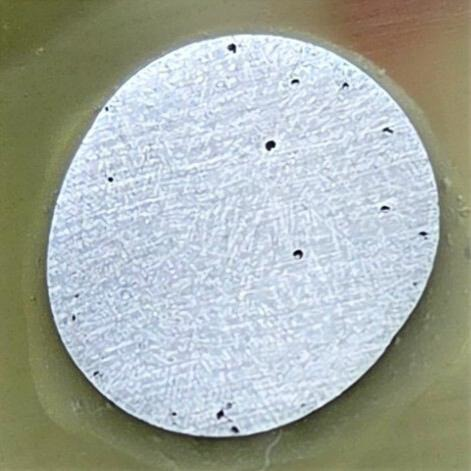
\includegraphics[width=\textwidth]{figs/A1_before.jpg}
         \caption{}
     \end{subfigure}
     \hfill
     \begin{subfigure}[b]{0.22\textwidth}
         \centering
         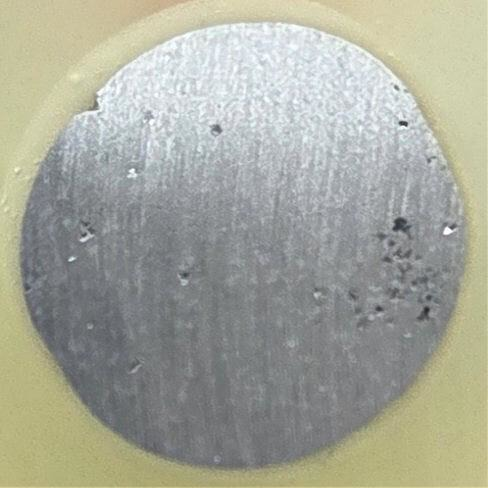
\includegraphics[width=\textwidth]{figs/A2_before.jpg}
         \caption{}
     \end{subfigure}
     \hfill
     \begin{subfigure}[b]{0.22\textwidth}
         \centering
         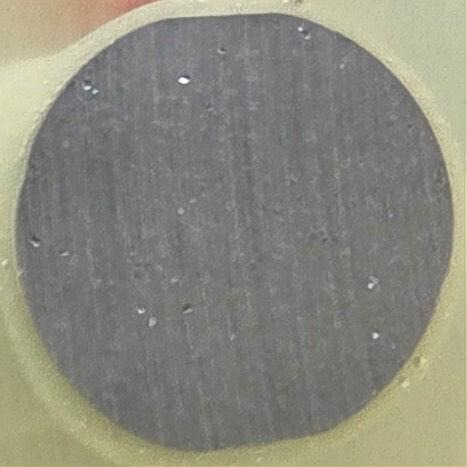
\includegraphics[width=\textwidth]{figs/A3_before.jpg}
         \caption{}
     \end{subfigure}
     \hfill
     \begin{subfigure}[b]{0.22\textwidth}
         \centering
         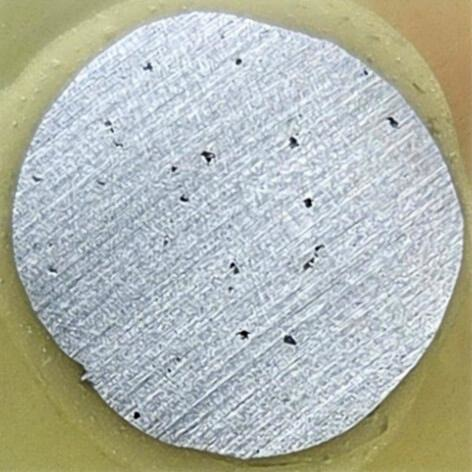
\includegraphics[width=\textwidth]{figs/A4_before.jpg}
         \caption{}
     \end{subfigure}
     \caption{Surface condition before measurements.}
     \label{fig:before_measurements}
\end{figure}

\begin{table}[htbp]
    \centering
    \small % Define a letra mais pequena
    \setlength{\tabcolsep}{25pt} % Aumenta a largura da tabela (espaço entre colunas)
    \caption{Chemical composition of the AC46000 aluminium alloy (wt\%)}
    \label{tab:AC46000_composition}
    \begin{tabular}{ll}
        \toprule
        Element & Content \\
        \midrule
        Si (Silicon)   & 8.00 -- 11.0      \\
        Cu (Copper)    & 2.00 -- 4.00      \\
        Fe (Iron)      & 0.00 -- 1.30      \\
        Others*        & < 4.50            \\
        Al (Aluminium) & Balance           \\
        \bottomrule
        \multicolumn{2}{l}{\footnotesize *Includes Zn, Mg, Mn, Ni, Pb, Ti, Sn, Cr.}
    \end{tabular}
\end{table}

The selected corrosion inhibitors are listed in Table~\ref{tab:inhibitor}, with a standard concentration of 0.005 M, except for those with lower saturation limits. Sodium chloride (NaCl) at 0.05 M was used as the electrolyte. This concentration is commonly chosen because it provides high conductivity, resulting in low solution impedance, and allows easy comparison with existing studies. The pH of each solution was also measured prior to experimentation.

\begin{table}[htbp]
    \centering
    \small % Letra mais pequena
    \setlength{\tabcolsep}{12pt} % Ajuste da largura (espaço entre colunas)
    \caption{Composition of the solutions for testing the effectiveness of the inhibitors and respective pH values}
    \label{tab:inhibitor}
    \begin{tabular}{lcc}
        \toprule
        Solution Composition & \begin{tabular}[c]{@{}c@{}}Concentration of\\ the reagent\end{tabular} & pH \\
        \midrule
        1. NaCl 0.05 M                           & ---       & 7.38 \\
        2. NaCl 0.05 M + NaVO$_3$                & 0.005 M   & 7.41 \\
        3. NaCl 0.05 M + Na$_2$MoO$_4$           & 0.005 M   & 6.70 \\
        4. NaCl 0.05 M + 2-mercaptobenzothiazole & Saturated & 5.67 \\
        \bottomrule
    \end{tabular}
\end{table}

EIS measurements were then performed inside a Faraday cage using a Gamry Interface 1000 potentiostat linked to a computer and Gamry Framework v.6.33 and Echem Analyst v.6.33 software packages for data acquisition and analysis. Measurements were conducted at open circuit potential with a 10 mV sinusoidal perturbation over a frequency range of 100 kHz to 10 mHz, using 10 points per decade. For the initial measurement, the lower frequency limit was set to 100 mHz due to insufficient sample stability.

A conventional three-electrode configuration was used (Figure~\ref{fig:setup1} and~\ref{fig:setup2}), comprising a saturated calomel electrode (SCE) as the RE, a platinum foil as the CE, and the exposed AC46000 substrate as the WE. The working electrode surface area was 0.95~cm$^{2}$, determined using ImageJ software (Figure~\ref{fig:imagej}). Samples were immersed for a total duration of seven days, with EIS measurements collected at 0 h, 1 h, 4 h, 8 h, 24 h, 48 h, 72 h, 120 h, and 168 h. 
\begin{figure}[ht]
     \centering
     \begin{subfigure}[t]{0.3\textwidth}
         \centering
         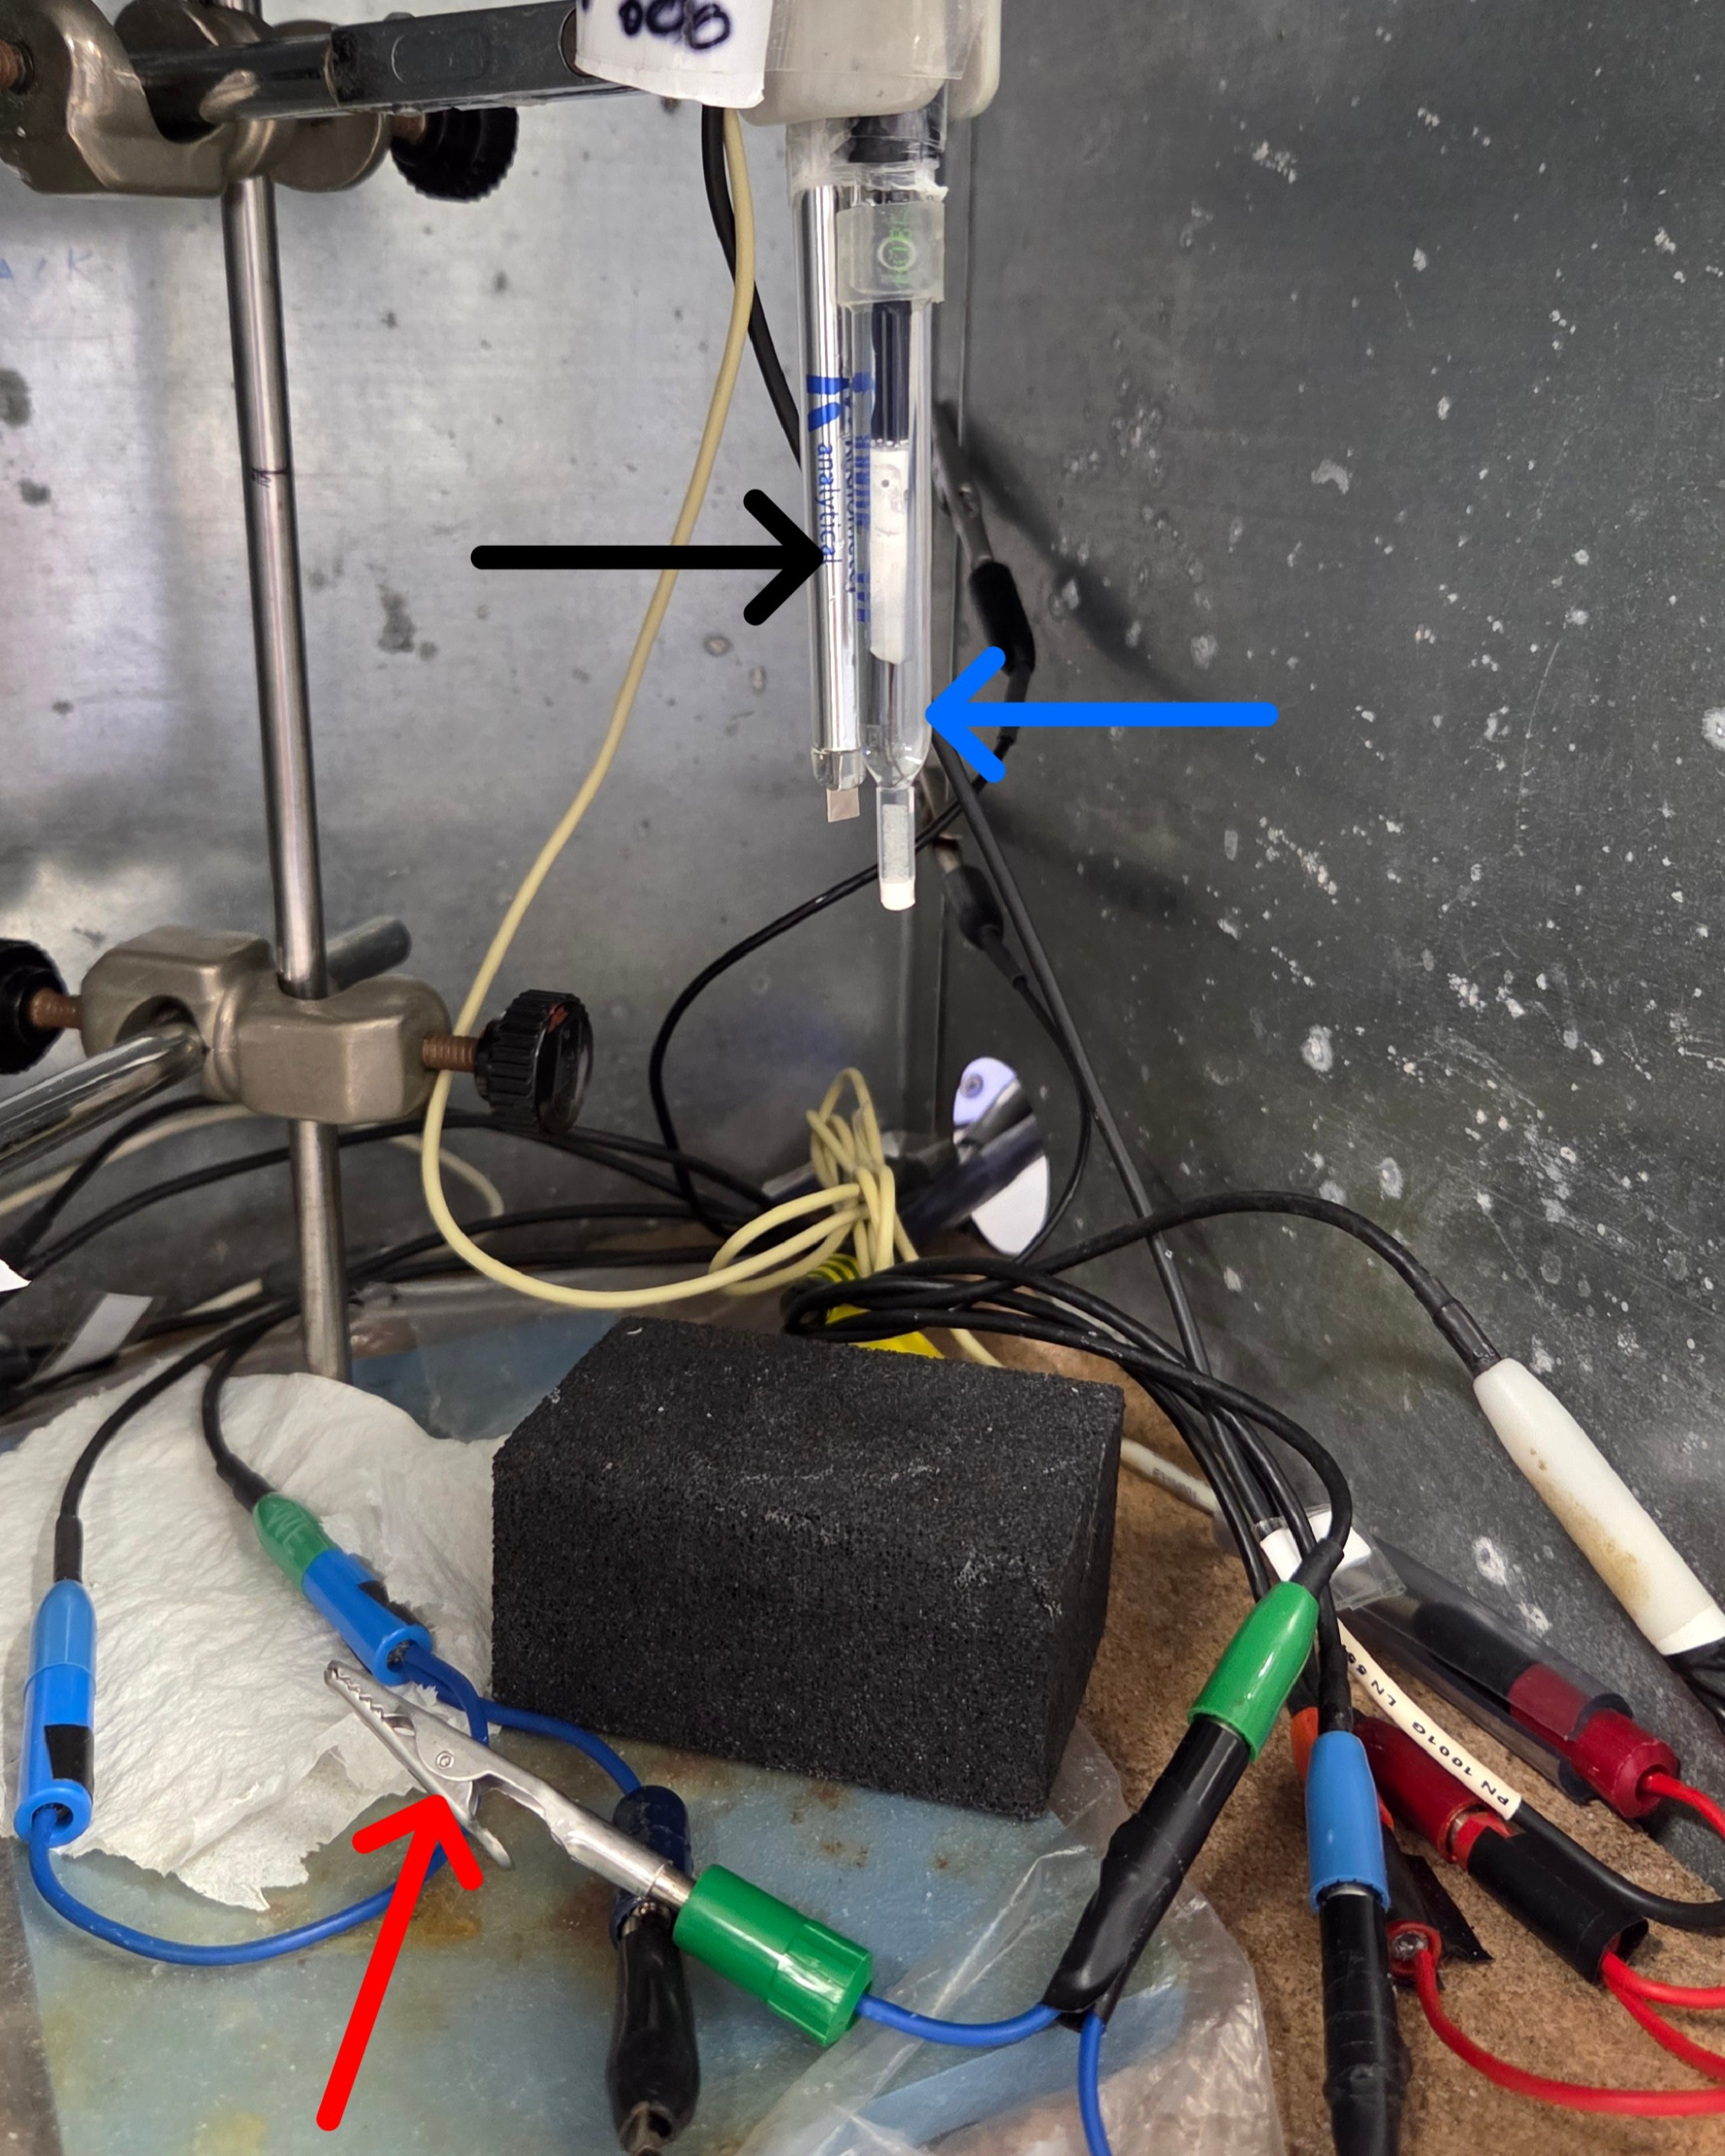
\includegraphics[width=\textwidth]{figs/setup1.JPG}
         \caption{Without the CE (black) and RE (blue) immersed and the WE (red) disconnected.}
         \label{fig:setup1}
     \end{subfigure}
     \hfill
     \begin{subfigure}[t]{0.3\textwidth}
         \centering
         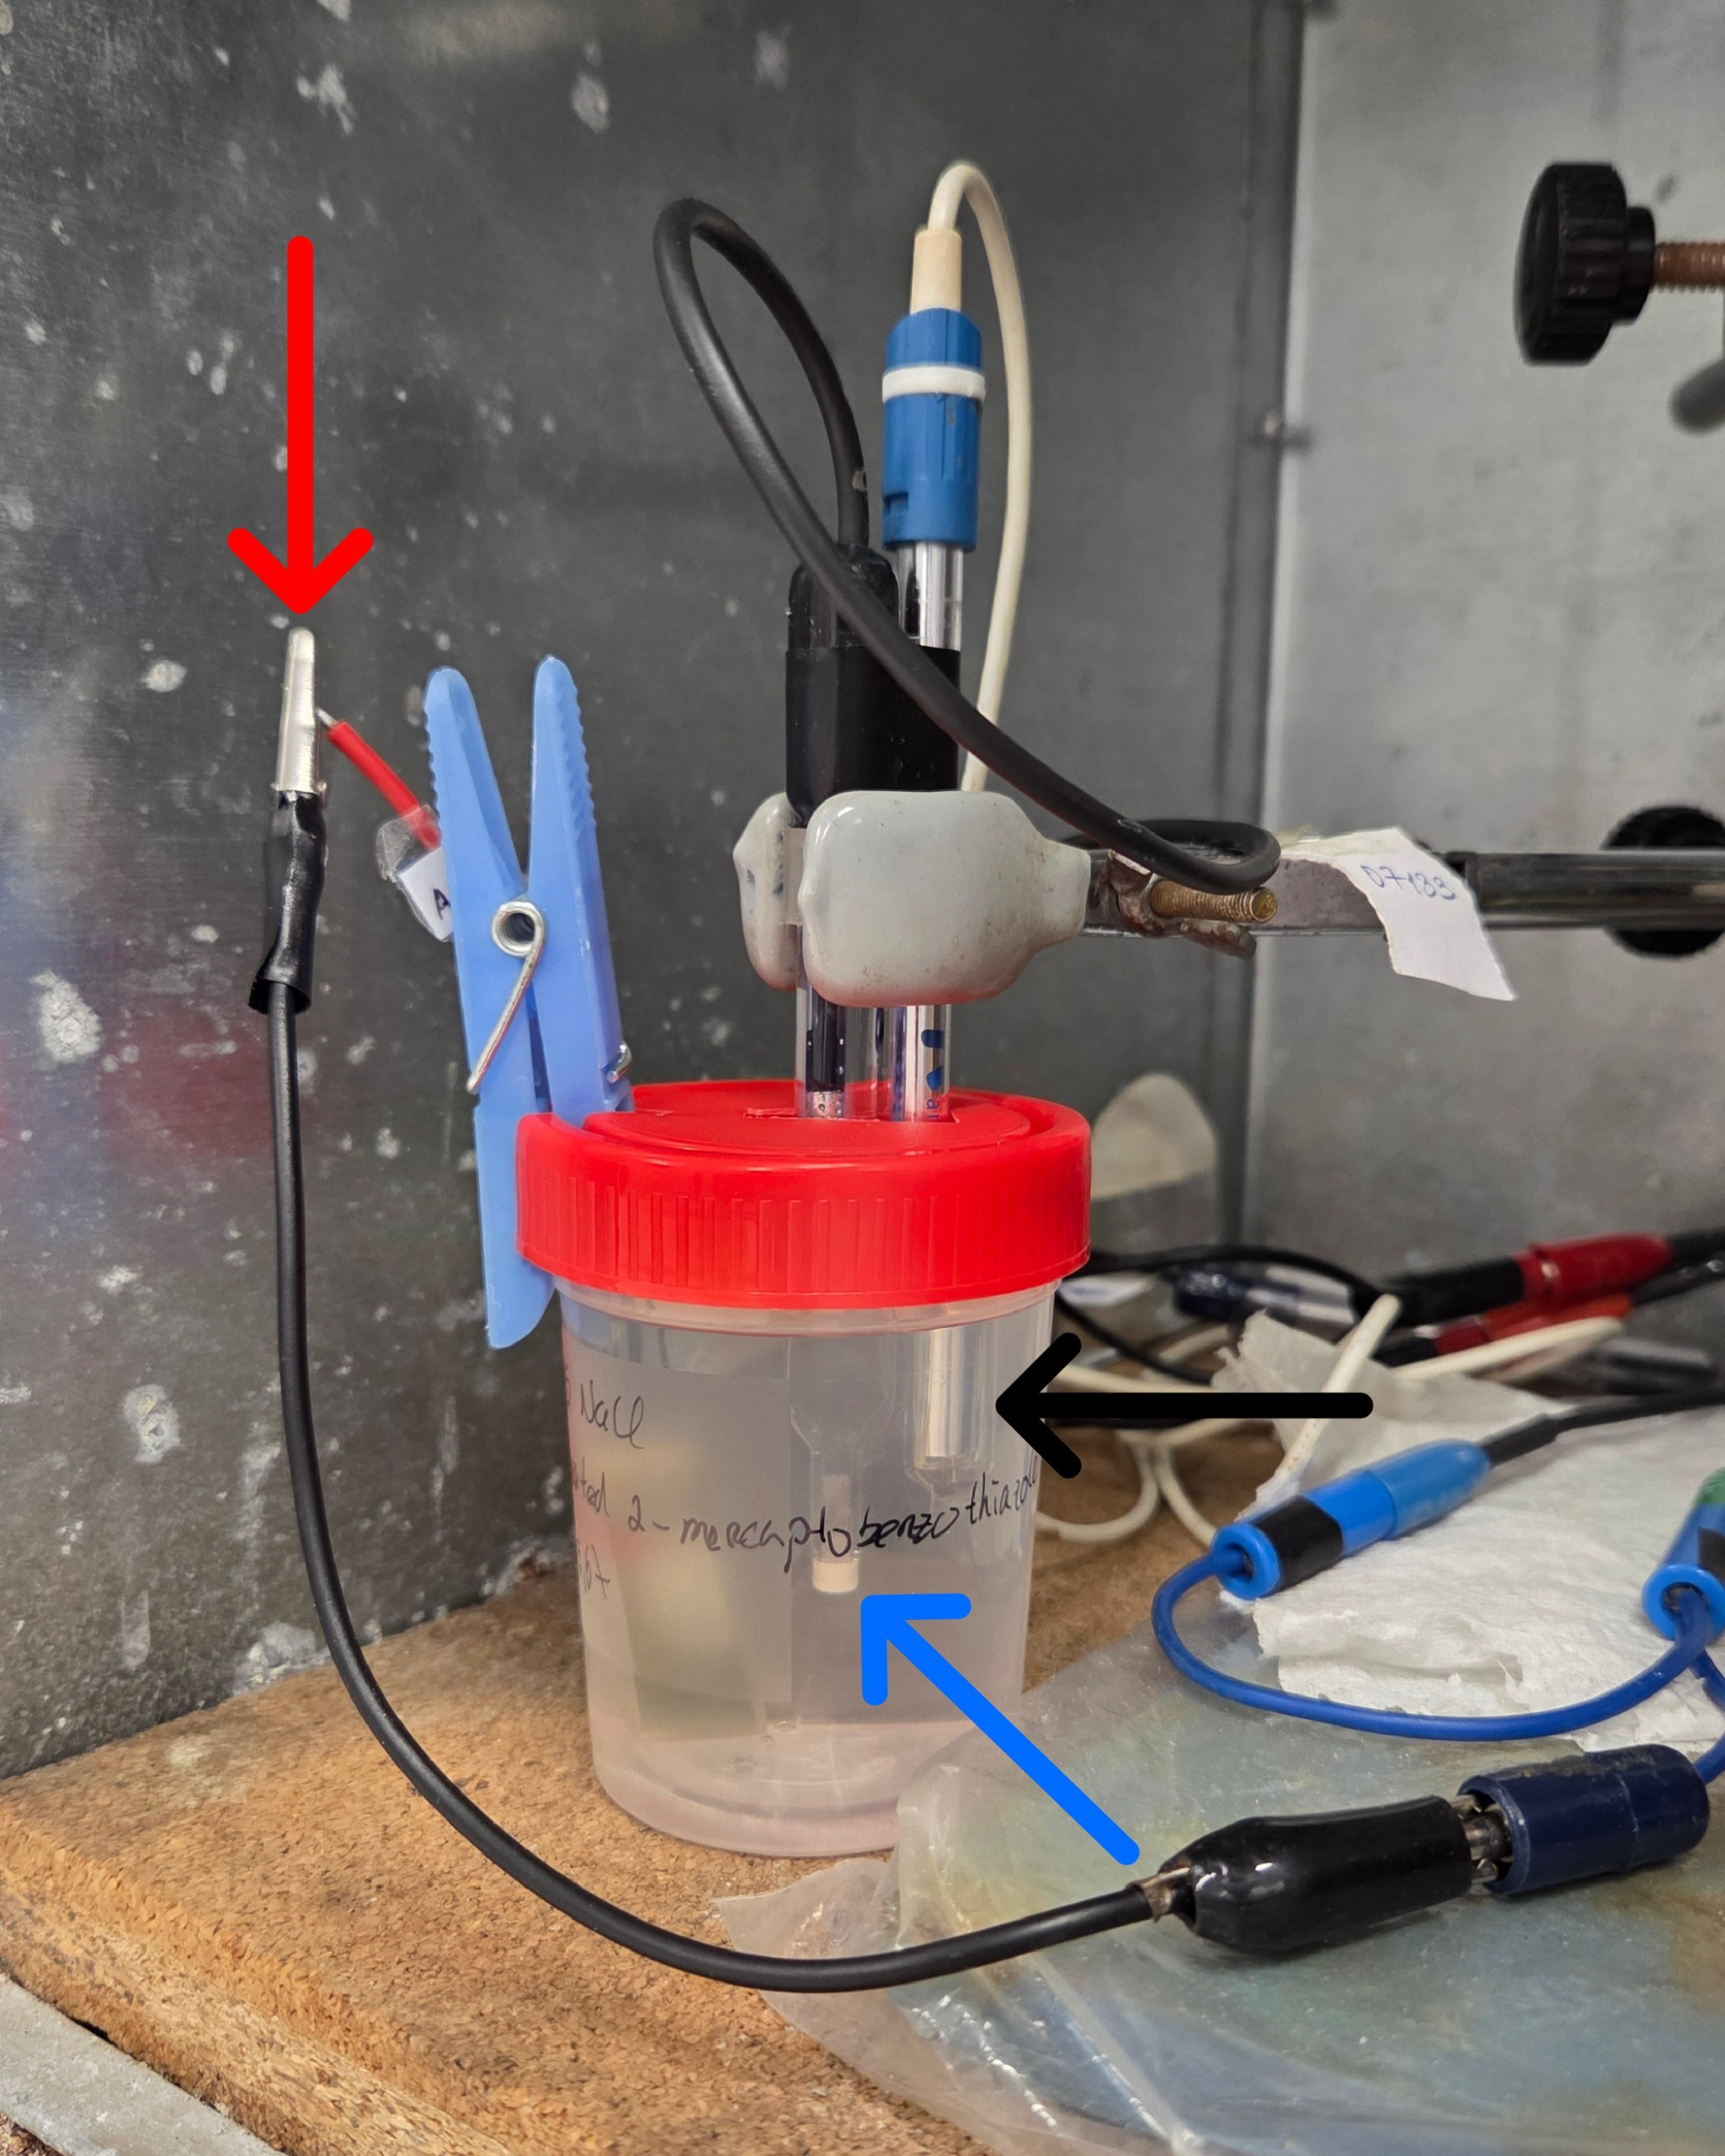
\includegraphics[width=\textwidth]{figs/setup2.JPG}
         \caption{With the electrodes immersed and the WE electrically connected to the metal surface.}
         \label{fig:setup2}
     \end{subfigure}
     \hfill
     \begin{subfigure}[t]{0.3\textwidth}
         \centering
         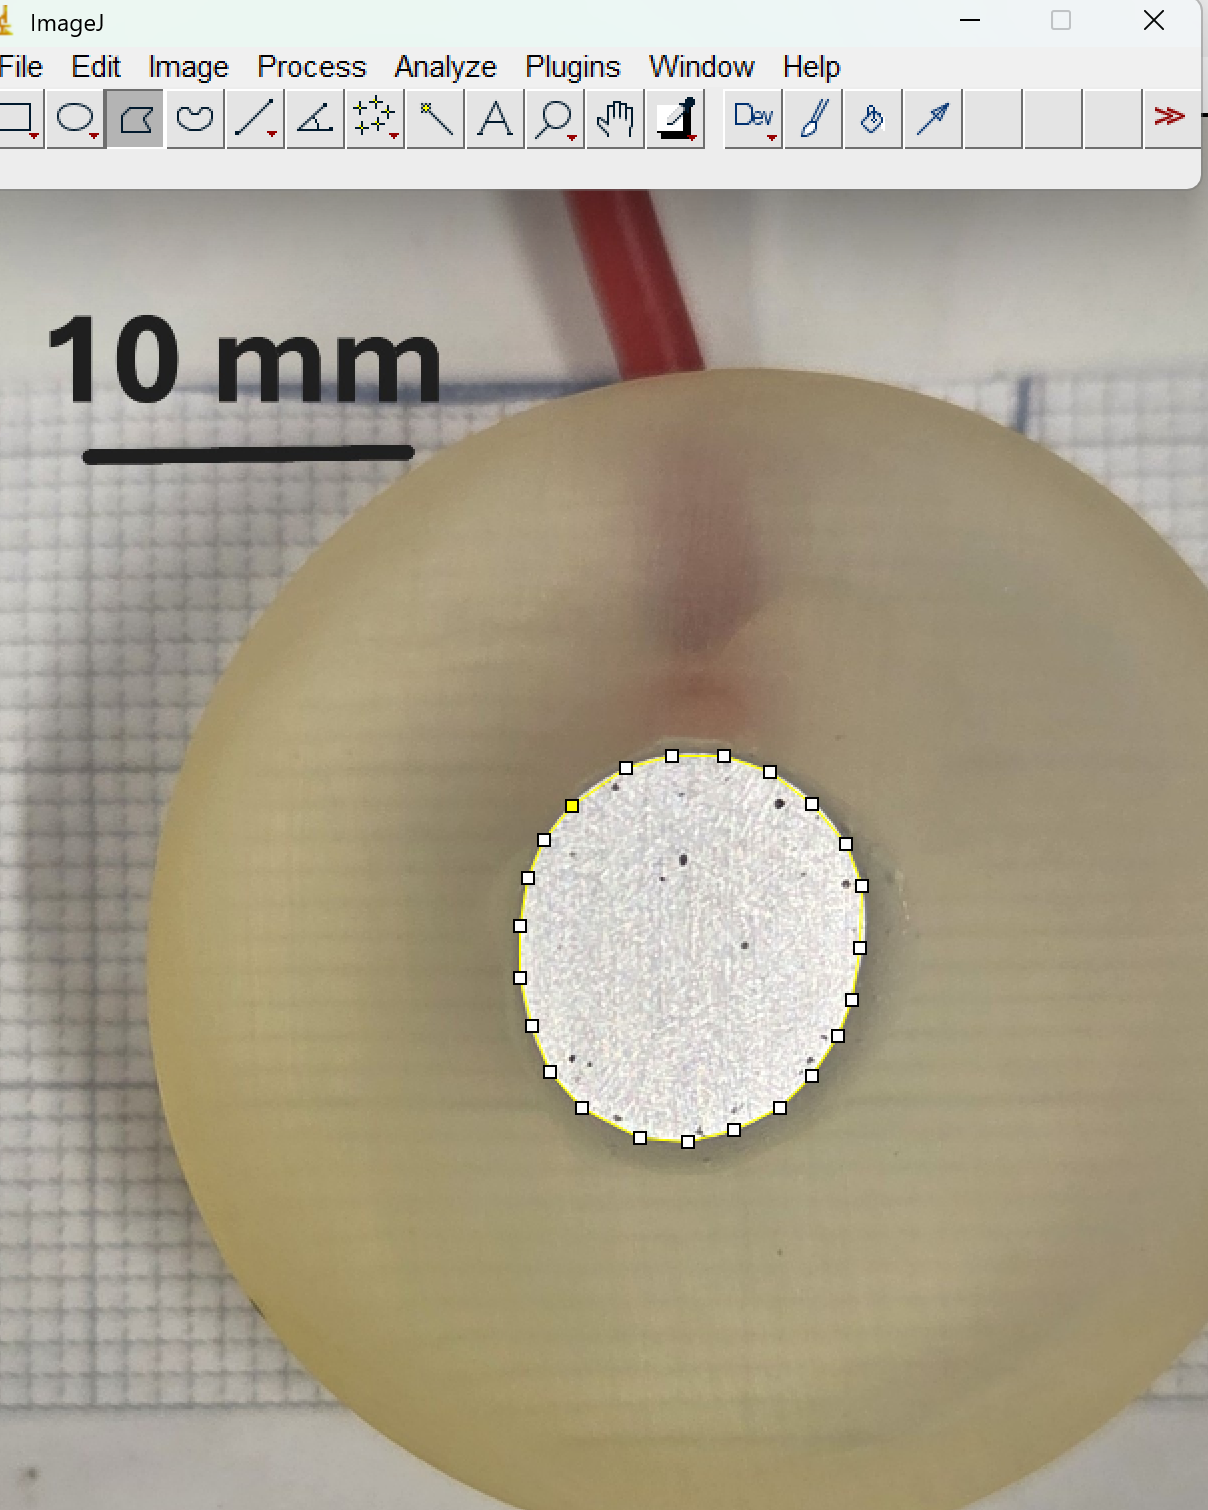
\includegraphics[width=\textwidth]{figs/Imagej.png}
         \caption{Determination of the exposed working electrode area using ImageJ software.}
         \label{fig:imagej}
     \end{subfigure}
     
     \caption{Electrochemical cell setup and working electrode area determination prior to EIS measurements.}
     \label{fig:setup}
\end{figure}



\chapter{Results}
The EIS results after 0 h and 168 h of immersion in NaCl electrolytes doped with different corrosion inhibitors are illustraded in Figure~\ref{Bodeplots1}

\begin{figure}[!ht]
     \centering
     \begin{subfigure}[b]{0.48\textwidth}
         \centering
         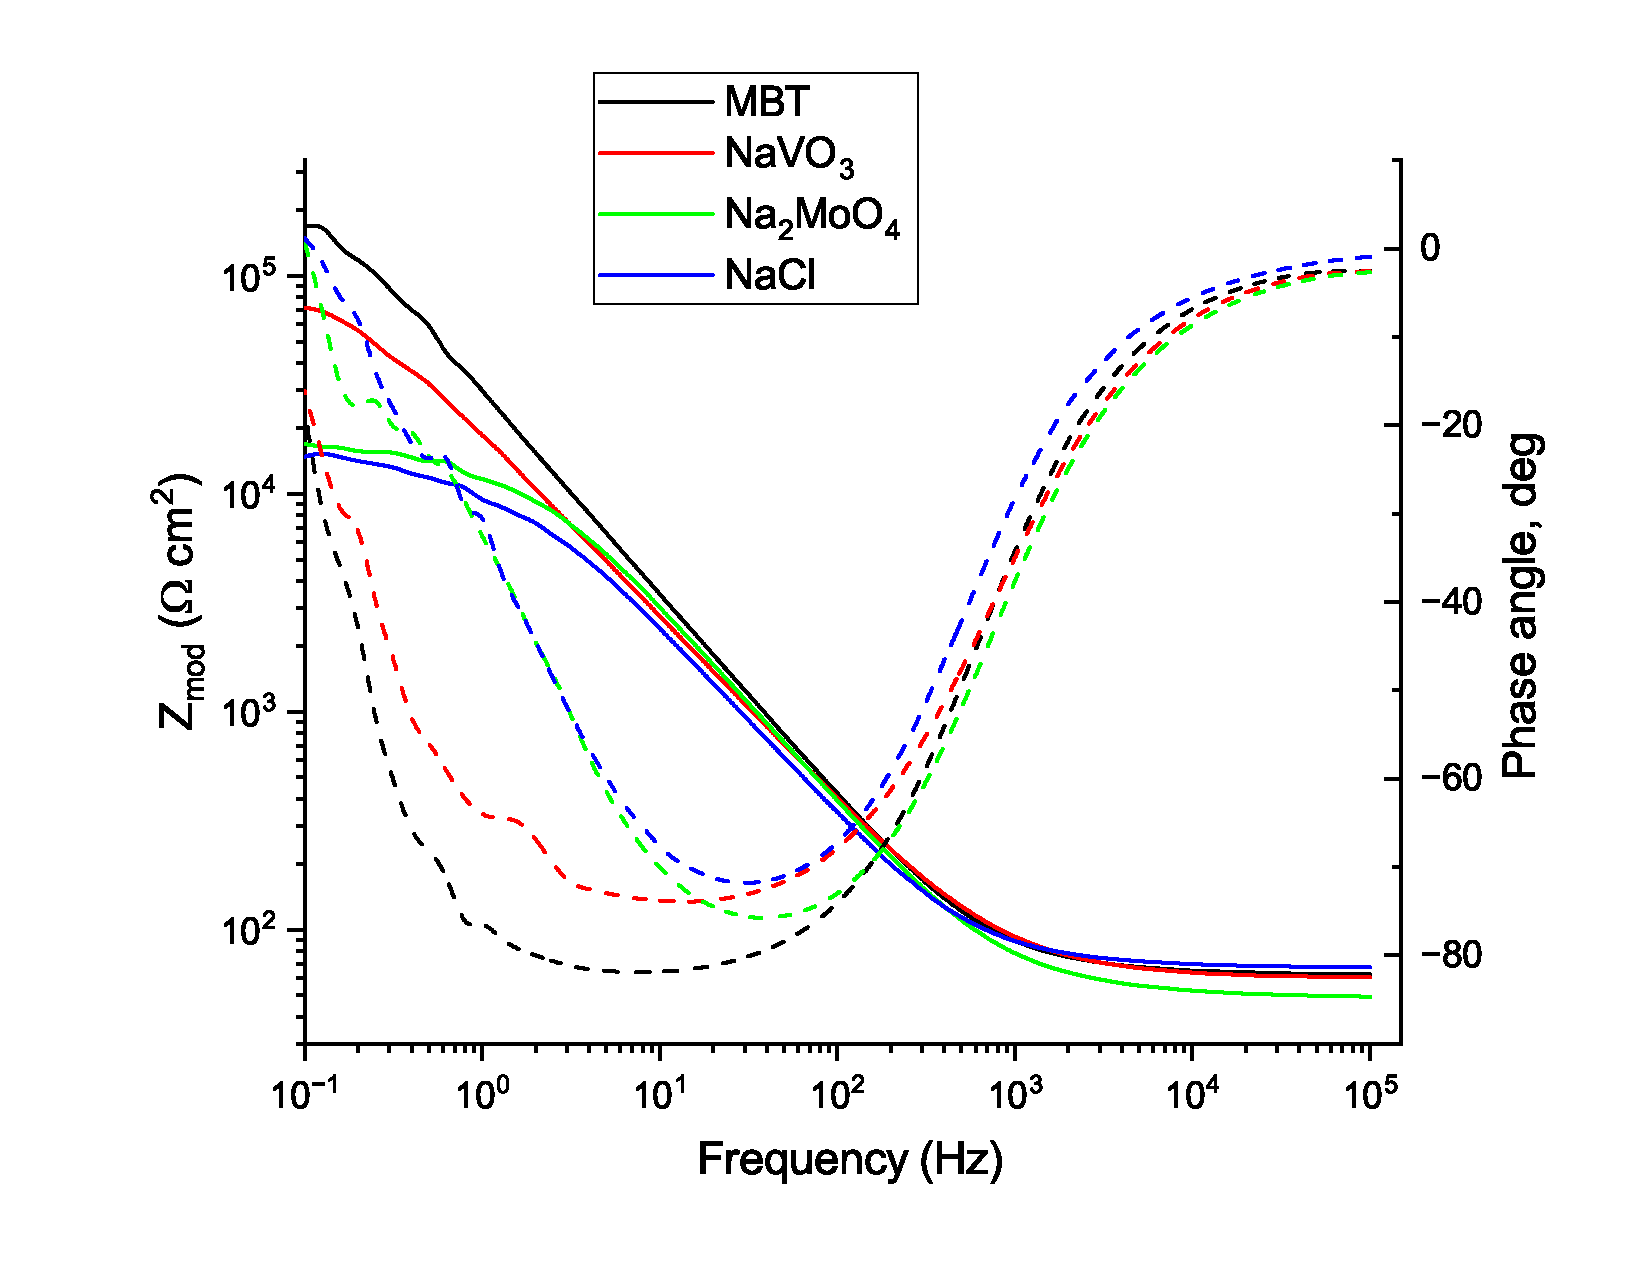
\includegraphics[width=\textwidth]{plots/Bode_0h.eps}
         \caption{}
         \label{fig:Bode0h}
     \end{subfigure}
     \hfill 
     \begin{subfigure}[b]{0.48\textwidth}
         \centering
         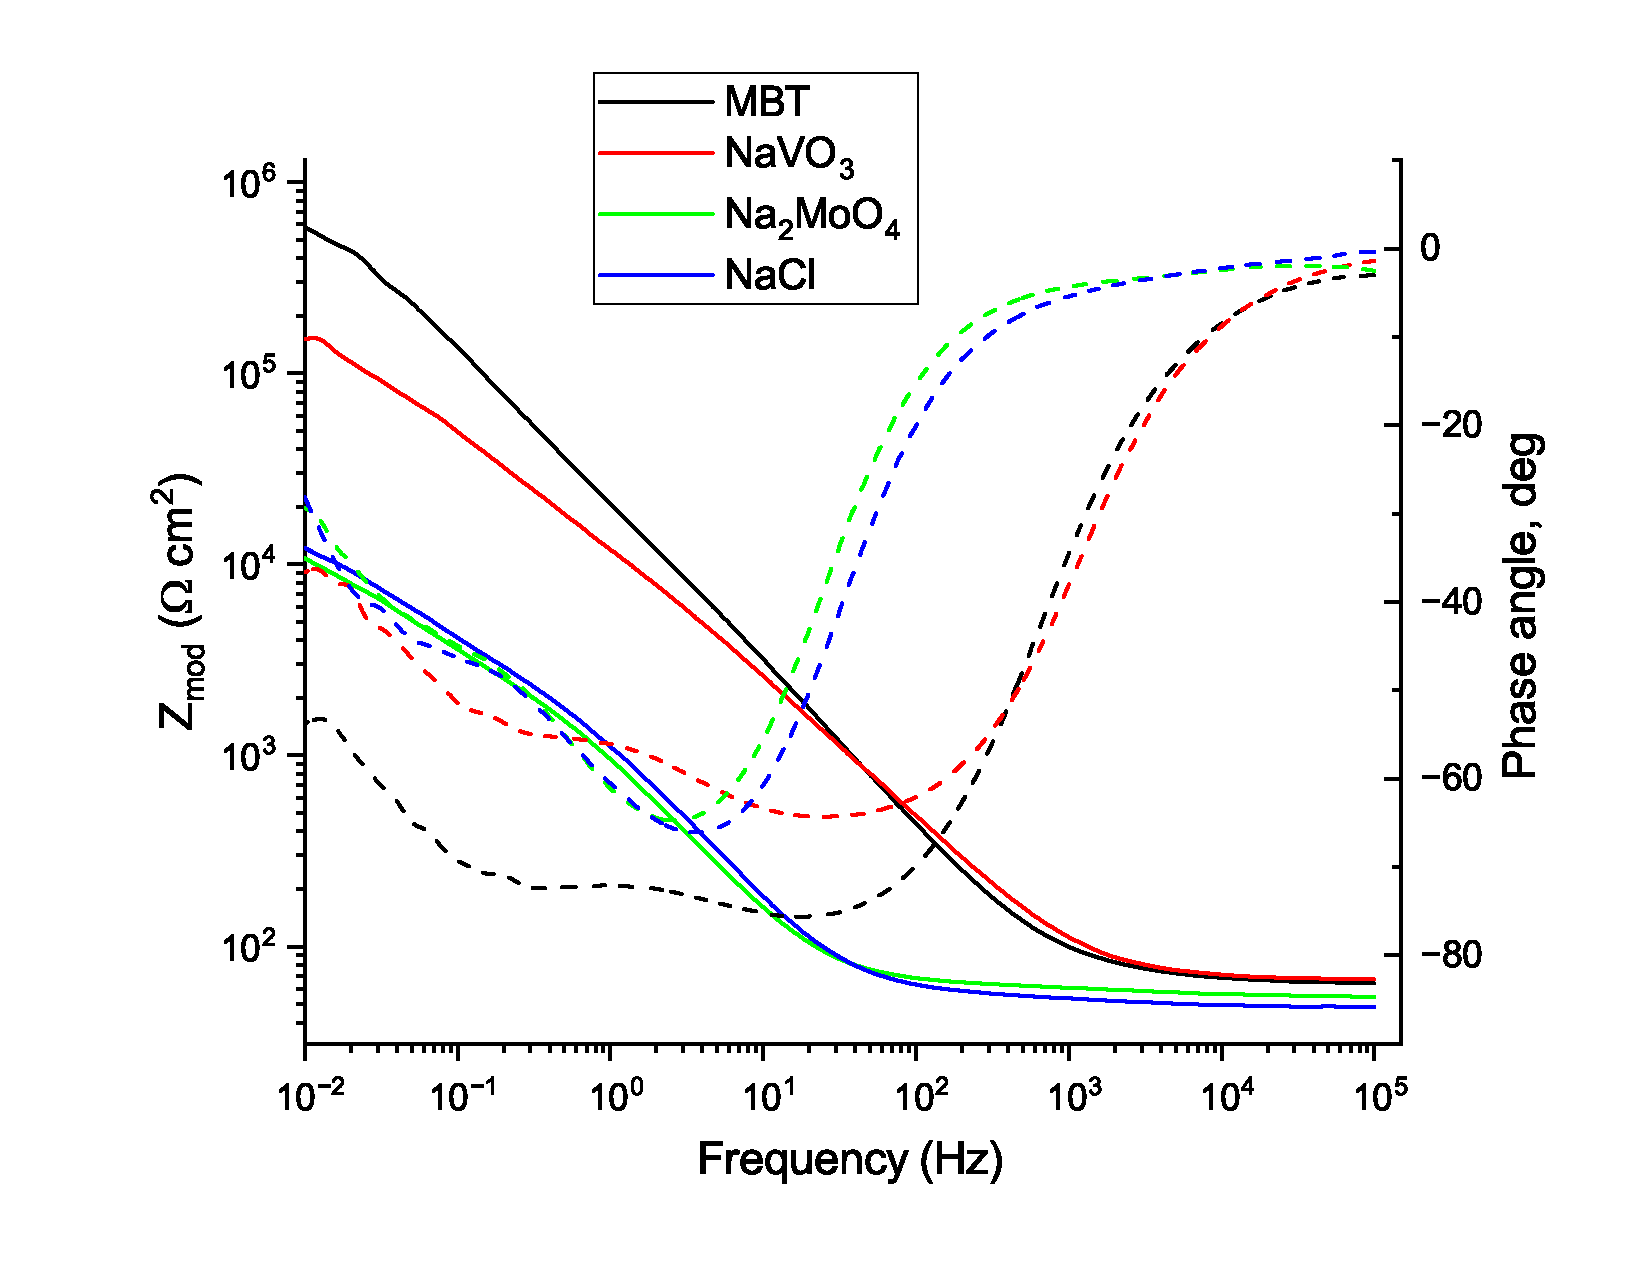
\includegraphics[width=\textwidth]{plots/Bode_168h.eps}
         \caption{}
         \label{fig:Bode168h}
     \end{subfigure}
     
     \vspace{0.5cm}

     \begin{subfigure}[b]{0.48\textwidth}
         \centering
         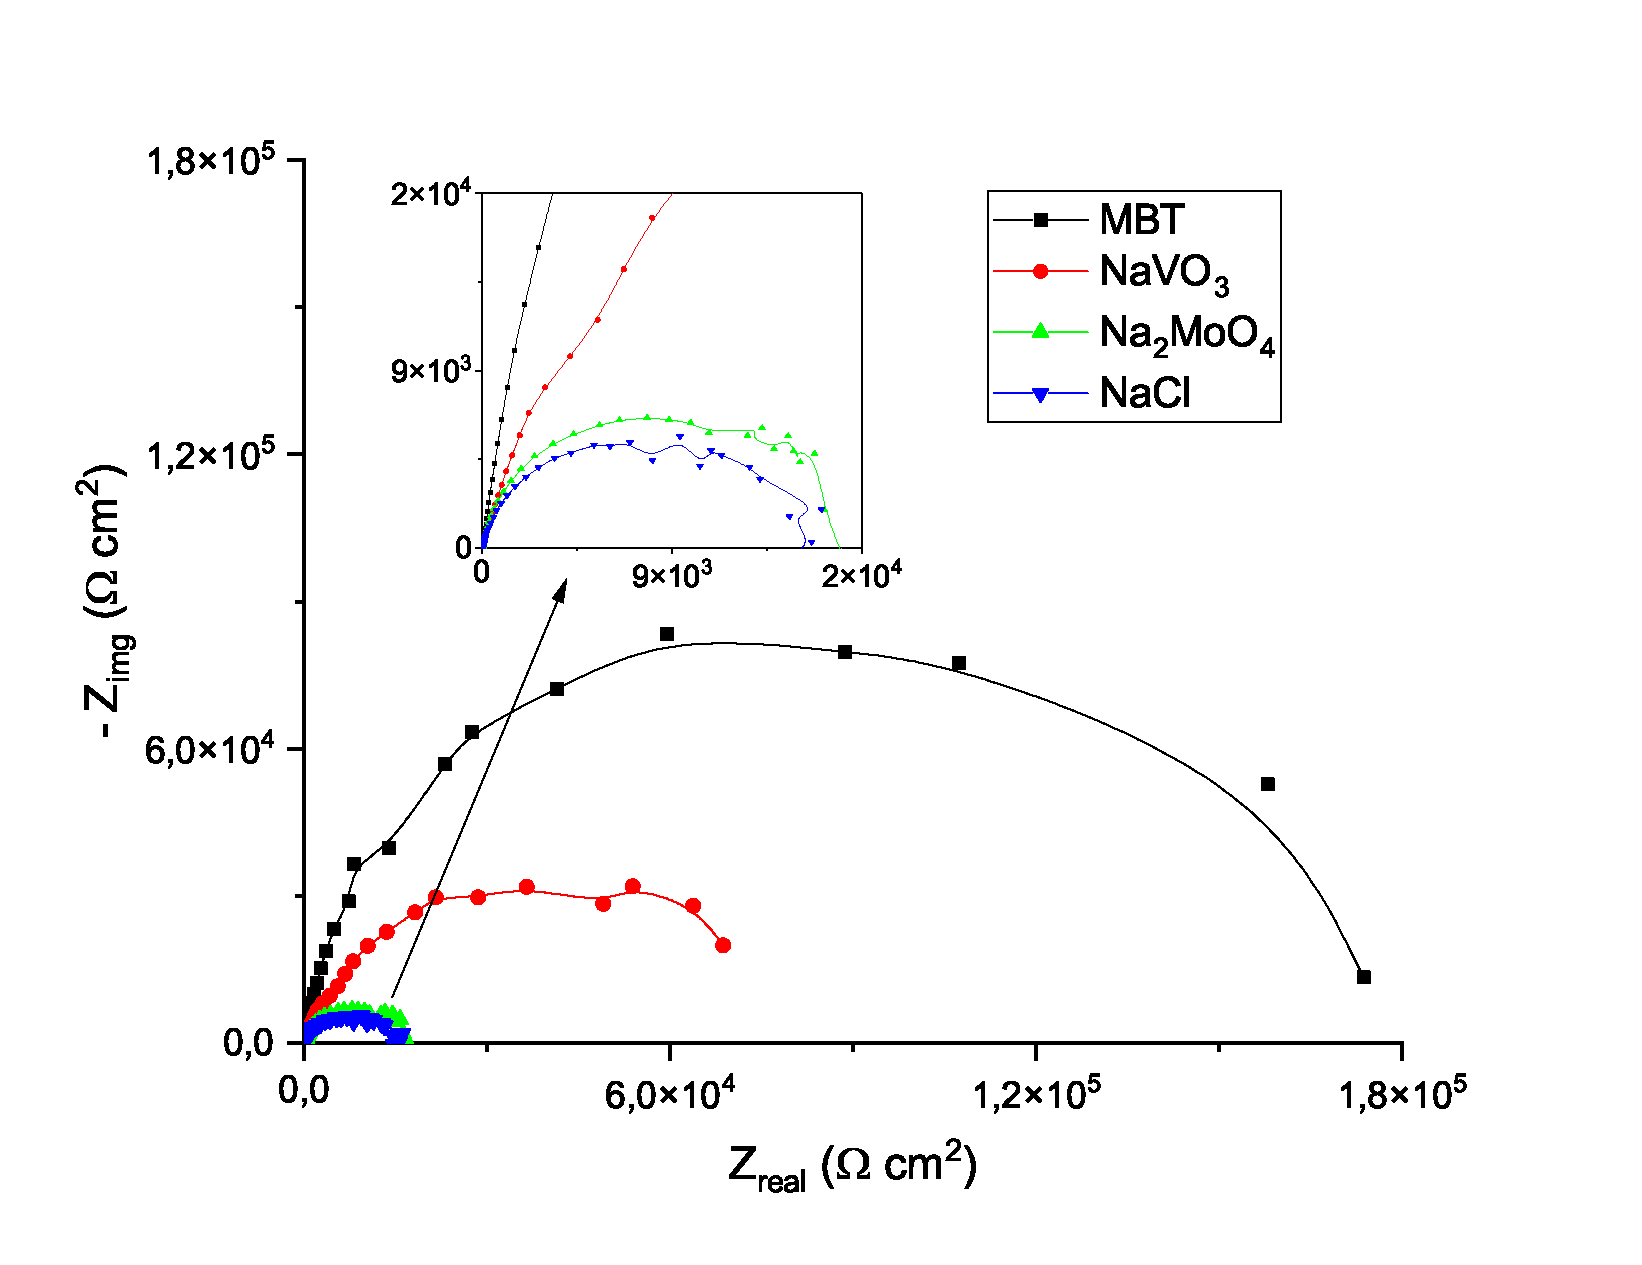
\includegraphics[width=\textwidth]{plots/Nyquist_0h_3.eps}
         \caption{}
         \label{fig:Nyquist0h}
     \end{subfigure}
     \hfill
     \begin{subfigure}[b]{0.48\textwidth}
         \centering
         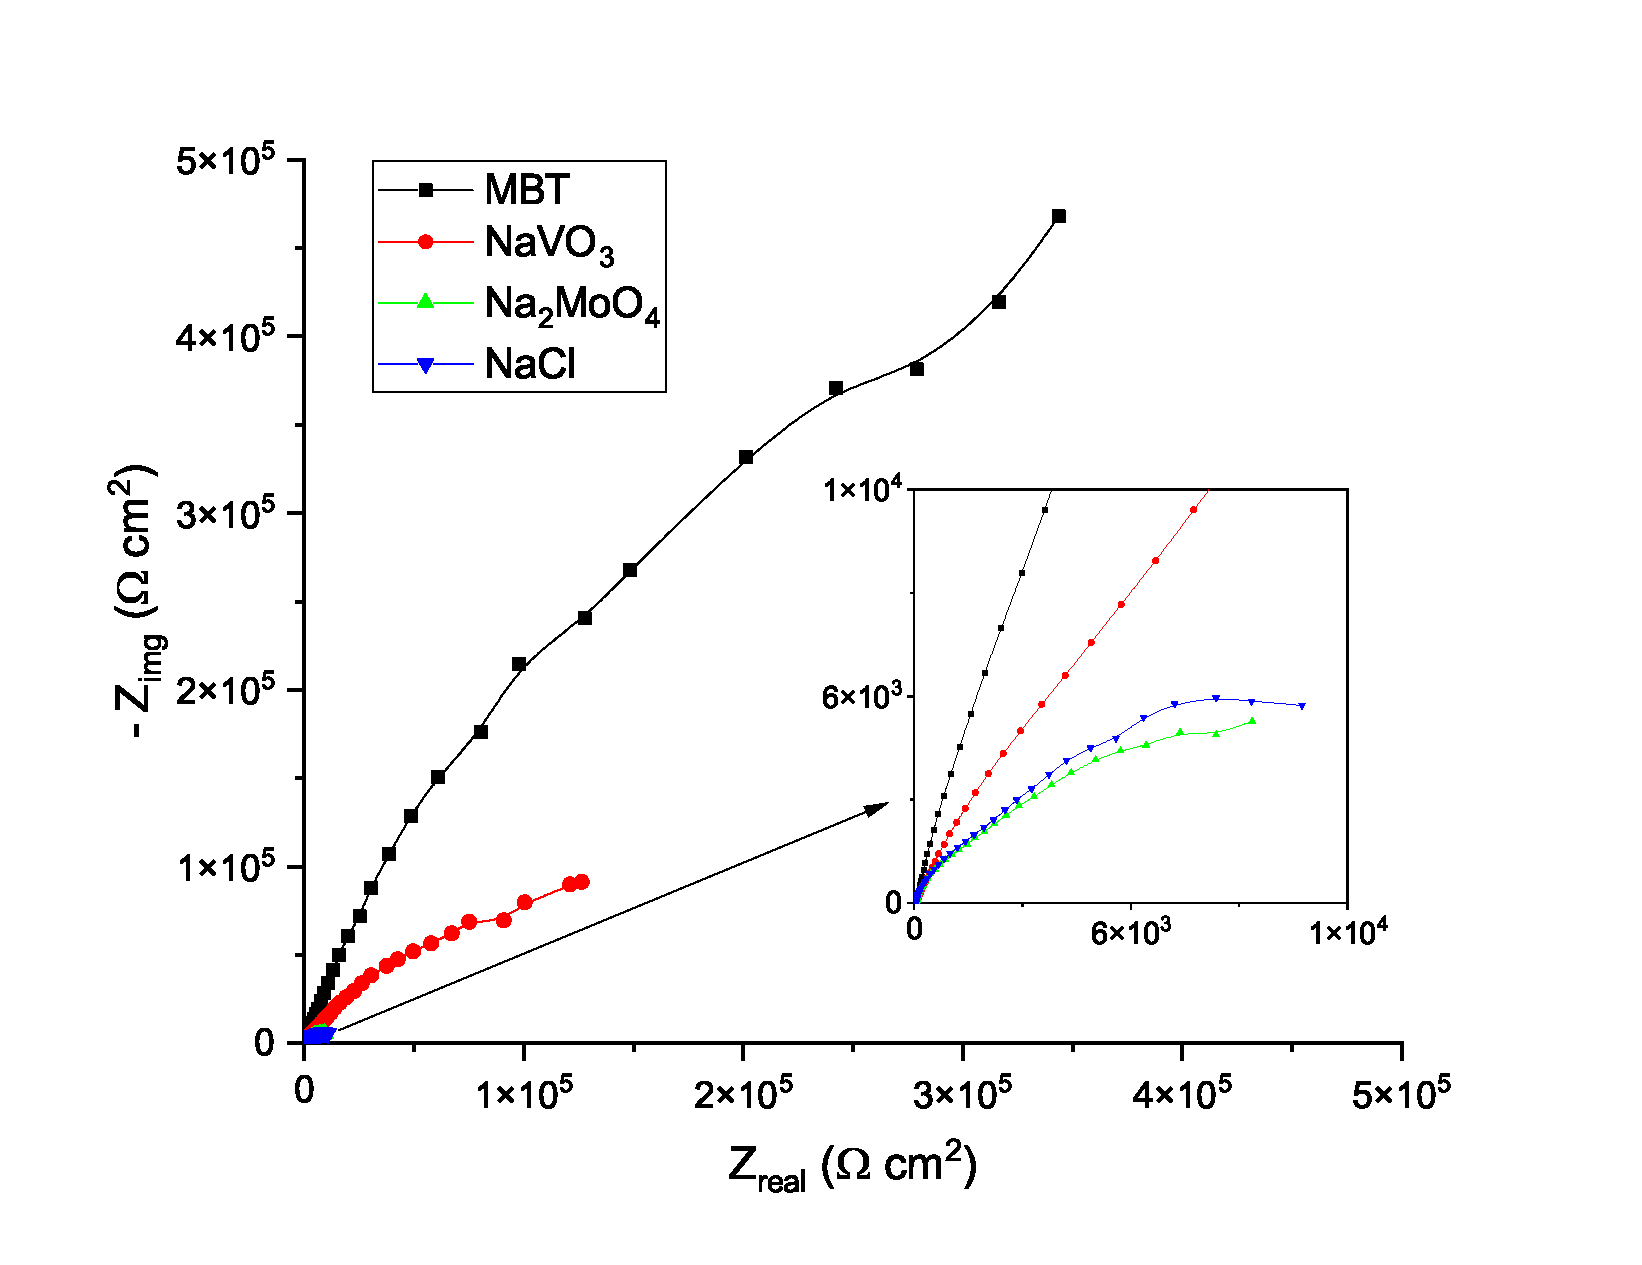
\includegraphics[width=\textwidth]{plots/Nyquist_168h_3.eps}
         \caption{}
         \label{fig:Nyquist168h}
     \end{subfigure}
     \caption{(a) and (b) Bode plots obtained for AC46000 after 0 h and 168h of immersion in 0.05 M NaCl with and without inhibitors; (c) and (d) Nyquist plots obtained for the same conditions.}
     \label{Bodeplots1}
\end{figure}

The figures for the other hours (1h, 4h, 8h, 24h, 48h, 72h and 120h) are displayed in the appendix in Figure~\ref{Bodeplots2}. 

To better visualize the changes in OCP and processes of charge transfer, OCP and variation of the modulus of impedance were plotted against time in Figure~\ref{OCP_Imp}.

\begin{figure}[!ht]
     \centering
     \begin{subfigure}[b]{0.48\textwidth}
         \centering
         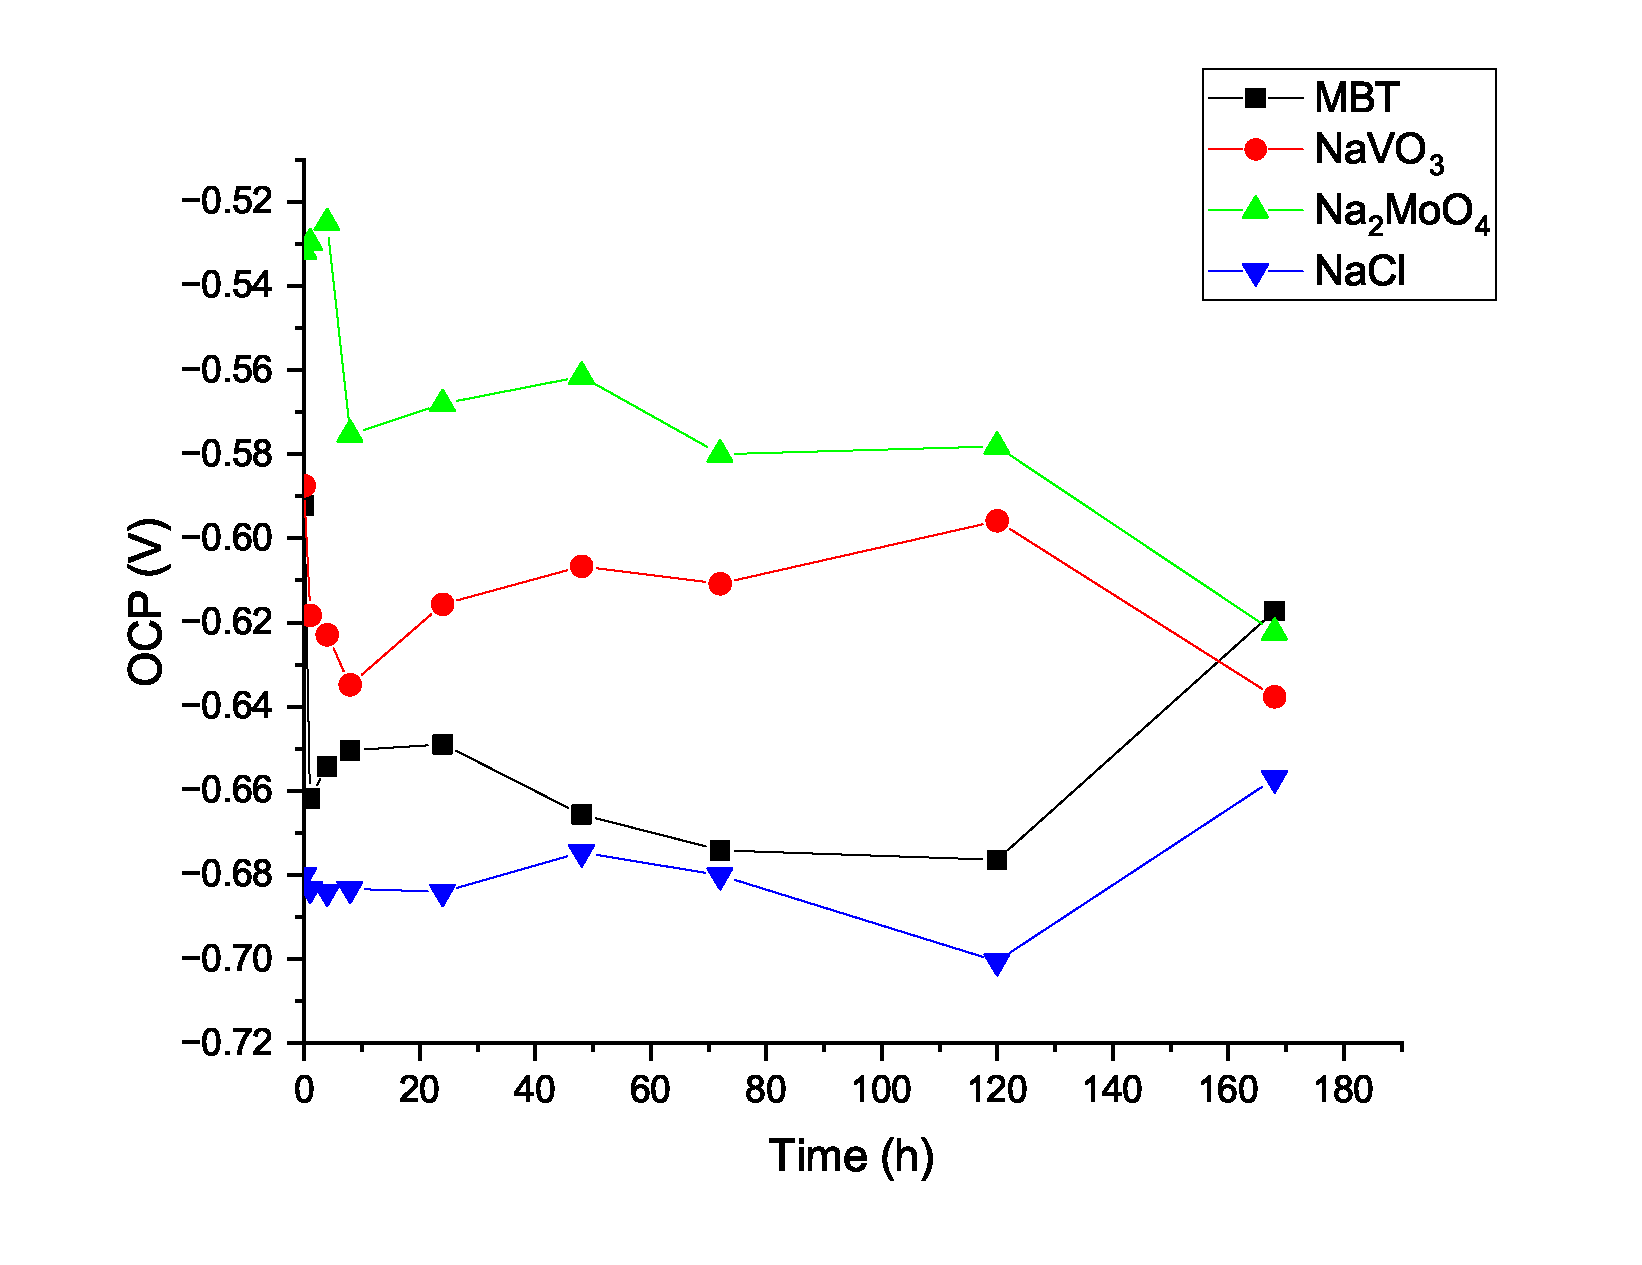
\includegraphics[width=\textwidth]{plots/OCP.eps}
         \caption{}
         \label{fig:OCP}
     \end{subfigure}
     \hfill 
     \begin{subfigure}[b]{0.48\textwidth}
         \centering
         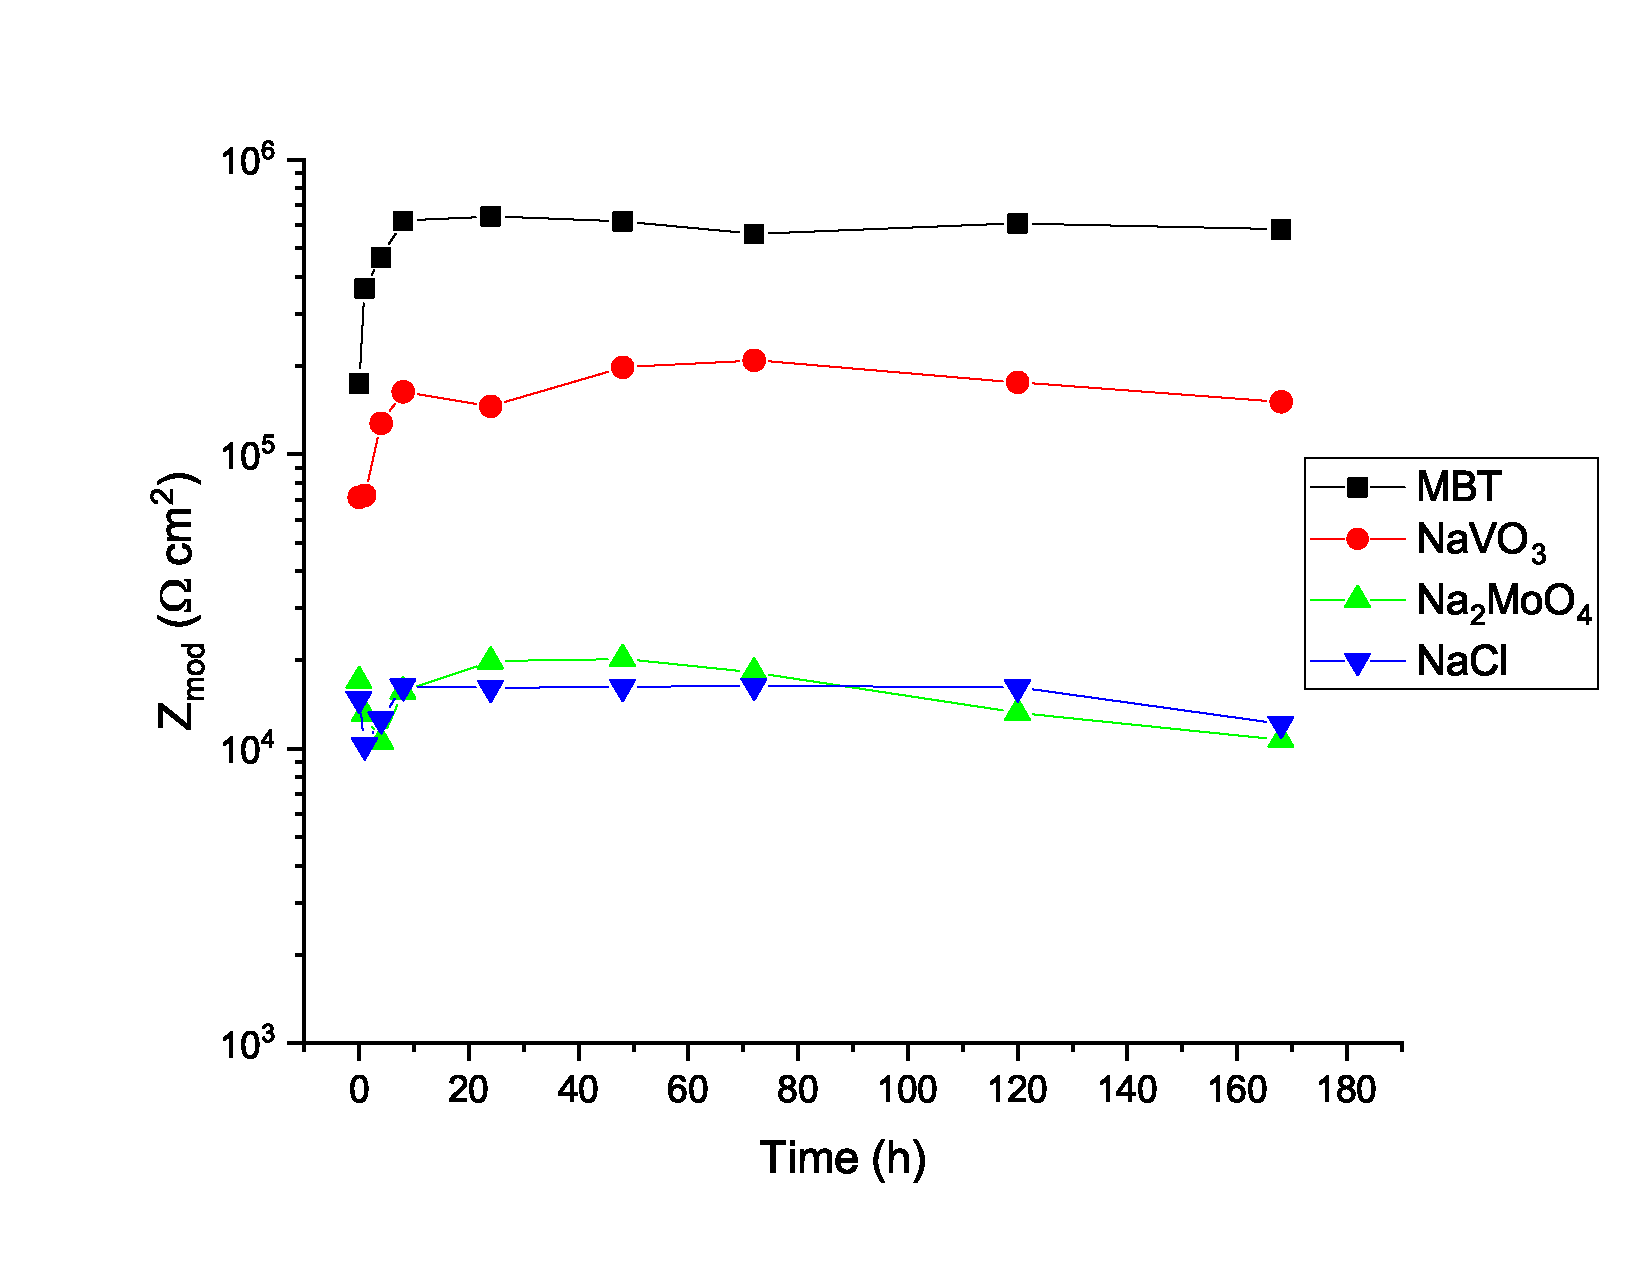
\includegraphics[width=\textwidth]{plots/Impedance3.eps}
         \caption{}
         \label{fig:Impedance}
     \end{subfigure}
     \caption{(a) Variation of OCP over time; (b) Variation of the modulus of impedance in the lowest frequency measured over time.} 
     \label{OCP_Imp}
\end{figure}

\begin{figure}[ht]
     \centering
     \begin{subfigure}[b]{0.22\textwidth}
         \centering
         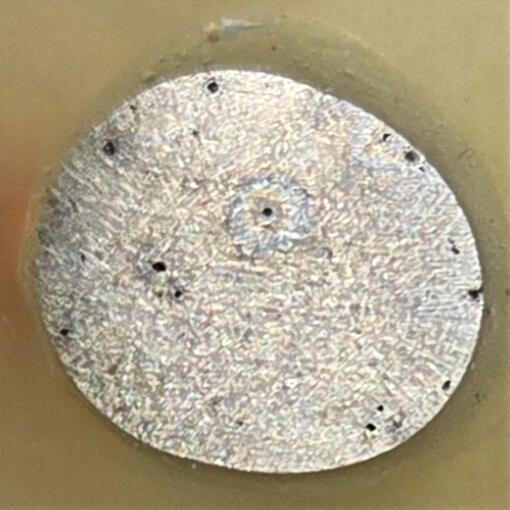
\includegraphics[width=\textwidth]{figs/A1_after.jpg}
         \caption{MBT}
         \label{A1}
     \end{subfigure}
     \hfill
     \begin{subfigure}[b]{0.22\textwidth}
         \centering
         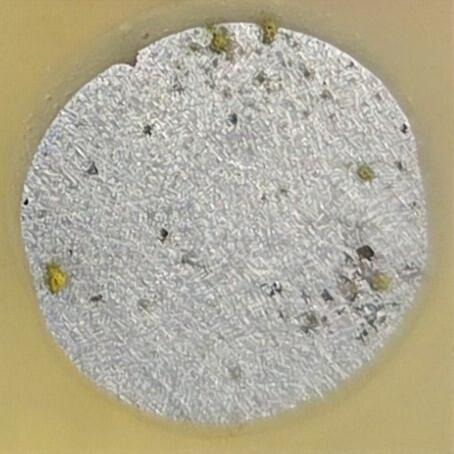
\includegraphics[width=\textwidth]{figs/A2_after.jpg}
         \caption{NaVO$_3$}
         \label{A2}
     \end{subfigure}
     \hfill
     \begin{subfigure}[b]{0.22\textwidth}
         \centering
         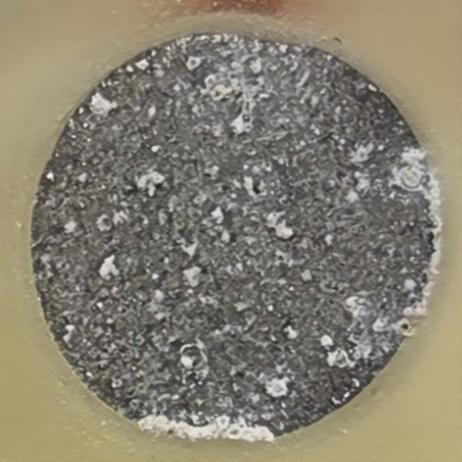
\includegraphics[width=\textwidth]{figs/A3_after.jpg}
         \caption{Na$_2$MoO$_4$}
         \label{A3}
     \end{subfigure}
     \hfill
     \begin{subfigure}[b]{0.22\textwidth}
         \centering
         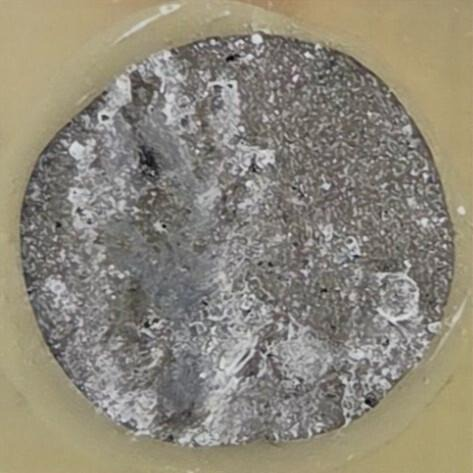
\includegraphics[width=\textwidth]{figs/A4_after.jpg}
         \caption{Uninhibited}
         \label{A4}
     \end{subfigure}
     \caption{Surface condition after 168h of immersion in 0.05 M NaCl with and without inhibitors.}
     \label{fig:after}
\end{figure}

\chapter{Discussion}

The EIS results (\Cref{fig:Bode0h,fig:Bode168h,fig:Nyquist0h,fig:Nyquist168h}) reveal clear differences in corrosion-inhibition performance over the 168 h immersion period. A consistent ranking emerges, with MBT providing the highest level of protection, followed by sodium metavanadate (NaVO$_3$), while sodium molybdate (Na$_2$MoO$_4$) performs comparably to the uninhibited NaCl electrolyte.

MBT- and NaVO$_3$-containing systems exhibit low-frequency impedance values approximately 1.5 and 1 order of magnitude higher, respectively, than those measured in the Na$_2$MoO$_4$ and uninhibited NaCl solutions, indicating superior corrosion resistance. This trend is confirmed by the Nyquist plots, where the latter systems display smaller semicircular arcs corresponding to lower charge-transfer resistance and poorer protective performance.

These findings contrast with earlier reports. \citet{Tedim2010} observed inferior performance of MBT relative to vanadates for AA2024, while \citet{Matsui2025} reported enhanced molybdate performance for an Al-Si-Cu alloy similar to AC46000. The discrepancy with the former study may stem from differences in alloy composition, as AA2024 contains higher magnesium content, whereas AC46000 is silicon-rich. In the latter case, the use of Mg-Al layered double hydroxides suggests a possible synergistic role of magnesium in the molybdate inhibition mechanism.

The time evolution of the low-frequency impedance, shown in the Bode plots (\Cref{fig:Impedance}), further supports these observations. For the NaCl and Na$_2$MoO$_4$ systems, the already low impedance values decrease slightly with immersion time, indicating progressive surface degradation and the absence of a stable protective layer. In contrast, the MBT and NaVO$_3$ systems maintain elevated impedance throughout exposure, consistent with sustained barrier properties. Such behavior is commonly associated with the formation of corrosion-product layers that hinder mass transport at the interface \cite{Tedim2014}.

At the initial immersion stage, all systems exhibit well-defined capacitive arcs, indicating charge-transfer-controlled behavior. After 168 h, deviations from ideal semicircular responses are observed across all samples, reflecting increasing interfacial complexity during prolonged exposure. This evolution is consistent with a transition toward mass-transfer-influenced processes, as reported by \citet{He2020} and \citet{Lazanas2023}.

Although the molybdate-containing samples show less negative OCP values up to approximately 160 h (\Cref{fig:OCP}), this does not necessarily indicate effective corrosion protection. The shift can result from increased cathodic currents associated with accelerated cathodic reactions, which promote localized dissolution of the aluminium matrix. As a result, the OCP may appear more positive despite ongoing corrosion. This underscores the distinction between thermodynamic indicators such as OCP and the kinetic resistance to corrosion captured by EIS and demonstrates that an OCP shift alone is insufficient to confirm protection without the formation of a stable, adherent surface film.

The electrochemical results are supported by post-test visual inspection of the samples (\Cref{fig:after}). MBT-treated surfaces remain largely uniform, with only a single visible corrosion pit. As reported by \citet{Garg2025}, MBT acts through a dual inhibition mechanism, protecting both the general aluminium surface and localized vulnerable sites. A thin molecular layer forms on the aluminium matrix, limiting overall oxidation, while preferential adsorption at intermetallic particles (IMPs) suppresses localized attack. Chloride ions assist this process by disrupting the native oxide film and exposing copper-rich IMP remnants, enabling MBT adsorption. The resulting protective layer inhibits the trenching and pitting that typically drive localized corrosion.

Metavanadate-treated samples display moderate surface modification, characterized by yellowish deposits composed of an insoluble compound referred to as aluminium vanadate. These deposits likely form from the reaction between aqueous metavanadate species (NaVO$_3$) and Al$^{3+}$ ions released by localized anodic dissolution of the aluminium matrix adjacent to cathodically active IMPs, where the cathodic reaction promotes an increase in local pH, as proposed by \citet{Kharitonov2019} and \citet{Huang2024}. 

In contrast, samples exposed to molybdate-containing and uninhibited NaCl solutions exhibit pronounced corrosion damage. The strong agreement between electrochemical measurements and visual observations confirms that, although interfacial complexity increases for all systems over time, effective inhibitors substantially limit surface degradation.







\chapter{Conclusion \& Future Work}
In this study, three corrosion inhibitors were evaluated in 0.05 M NaCl solutions to assess their corrosion protection efficiency using EIS. The results show a clear ranking of inhibitor performance: MBT > NaVO$_3$ > Na$_2$MoO$_4$.

To gain a deeper understanding of the inhibition mechanisms, particularly for sodium metavanadate, further surface analysis will be conducted. Scanning Electron Microscopy (SEM) and Energy Dispersive Spectroscopy (EDS) will be employed to characterize the aluminium-vanadate deposits and verify the formation of a passive layer, which contributes to the reduction of corrosion.

Building on these results, additional EIS studies will be performed across a broader range of inhibitors to determine whether MBT consistently provides the highest level of protection. The next candidates to be investigated include benzotriazole (BTA), L-cysteine, and 8-hydroxyquinoline. Both individual inhibitors and potential synergistic combinations will be explored.

With the completion of these activities, WP2 will be concluded. This will allow the project to progress to WP3, which focuses on substrate preparation and characterization, followed by WP4, where ZnAl layered double hydroxides (LDH) will be synthesized and subjected to anion exchange with the most effective corrosion inhibitor identified in this study. Further electrochemical and surface evaluations will then be performed.

Subsequently, WP5 will address corrosion performance assessment using EIS, as described in this report, along with complementary techniques such as the Scanning Vibrating Electrode Technique (SVET) to evaluate potential self-healing behavior.

Finally, for WP6 a complete multilayer protective system will be developed using anaphoretic coating techniques. This system will be applied to components with complex geometries, and its corrosion performance will be systematically evaluated.

\bibliographystyle{plainnat}
\bibliography{references}


\chapter*{Appendix}
\label{appendix}
\setcounter{figure}{0} 
\renewcommand{\thefigure}{A.\arabic{figure}} 


\begin{figure}[!ht]
     \centering
     \begin{subfigure}[b]{0.48\textwidth}
         \centering
         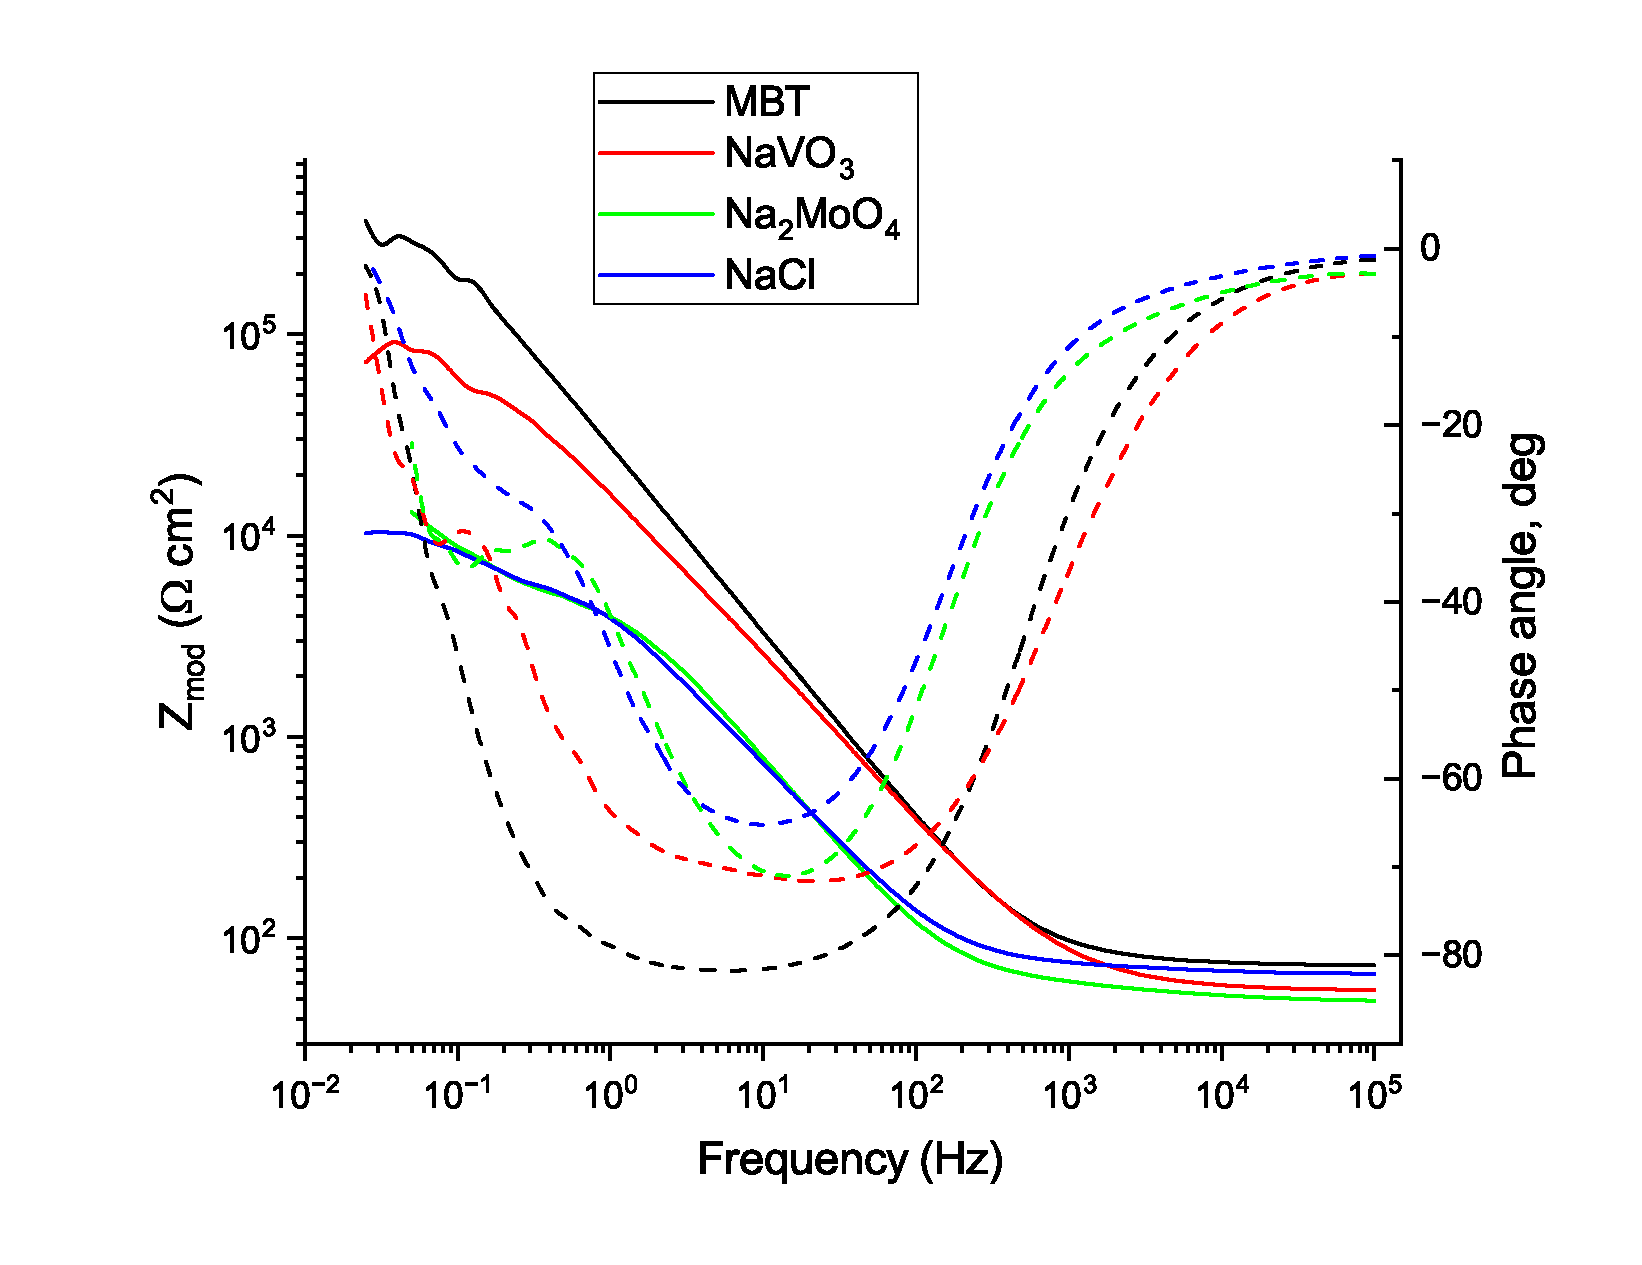
\includegraphics[width=\textwidth]{plots/Bode_1h.eps}
         \caption{}
         \label{fig:Bode1h}
     \end{subfigure}
     \hfill 
     \begin{subfigure}[b]{0.48\textwidth}
         \centering
         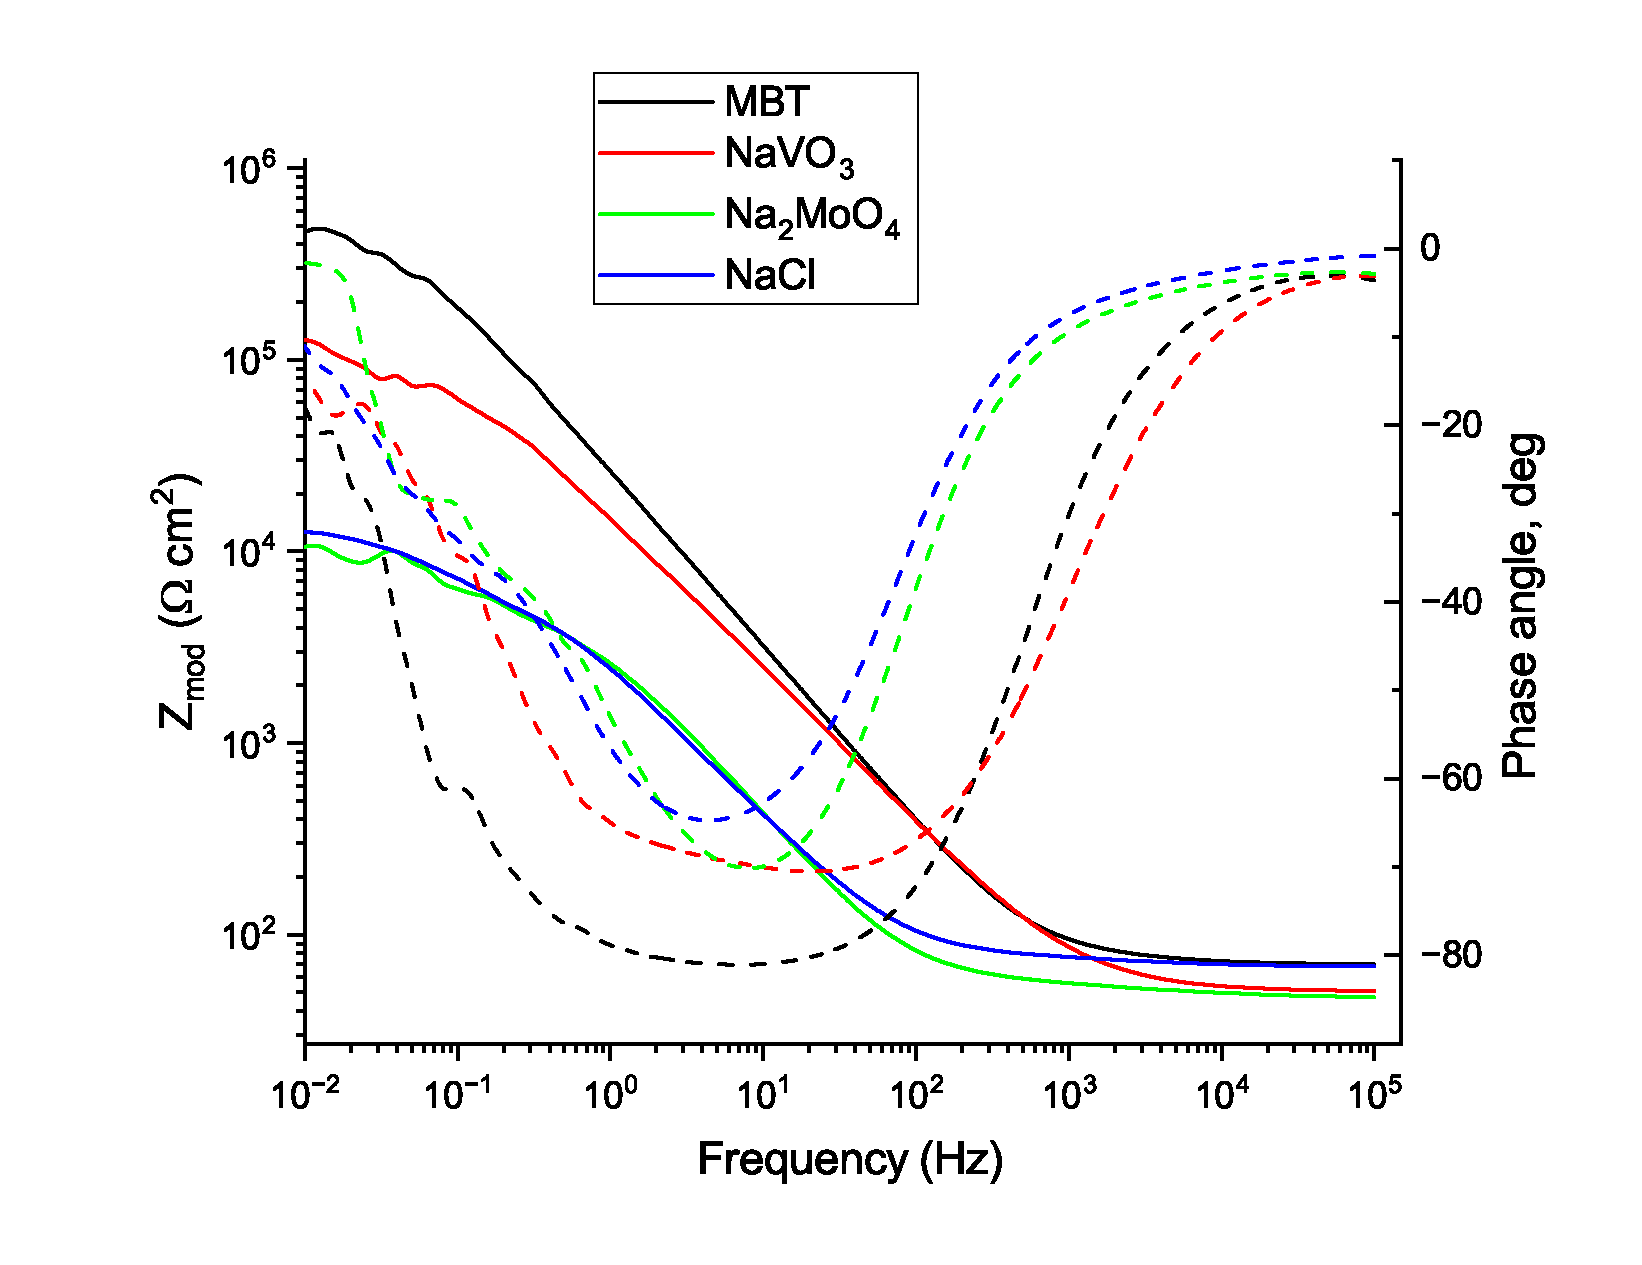
\includegraphics[width=\textwidth]{plots/Bode_4h.eps}
         \caption{}
         \label{fig:Bode4h}
     \end{subfigure}

     \vspace{0.5cm}

     \begin{subfigure}[b]{0.48\textwidth}
         \centering
         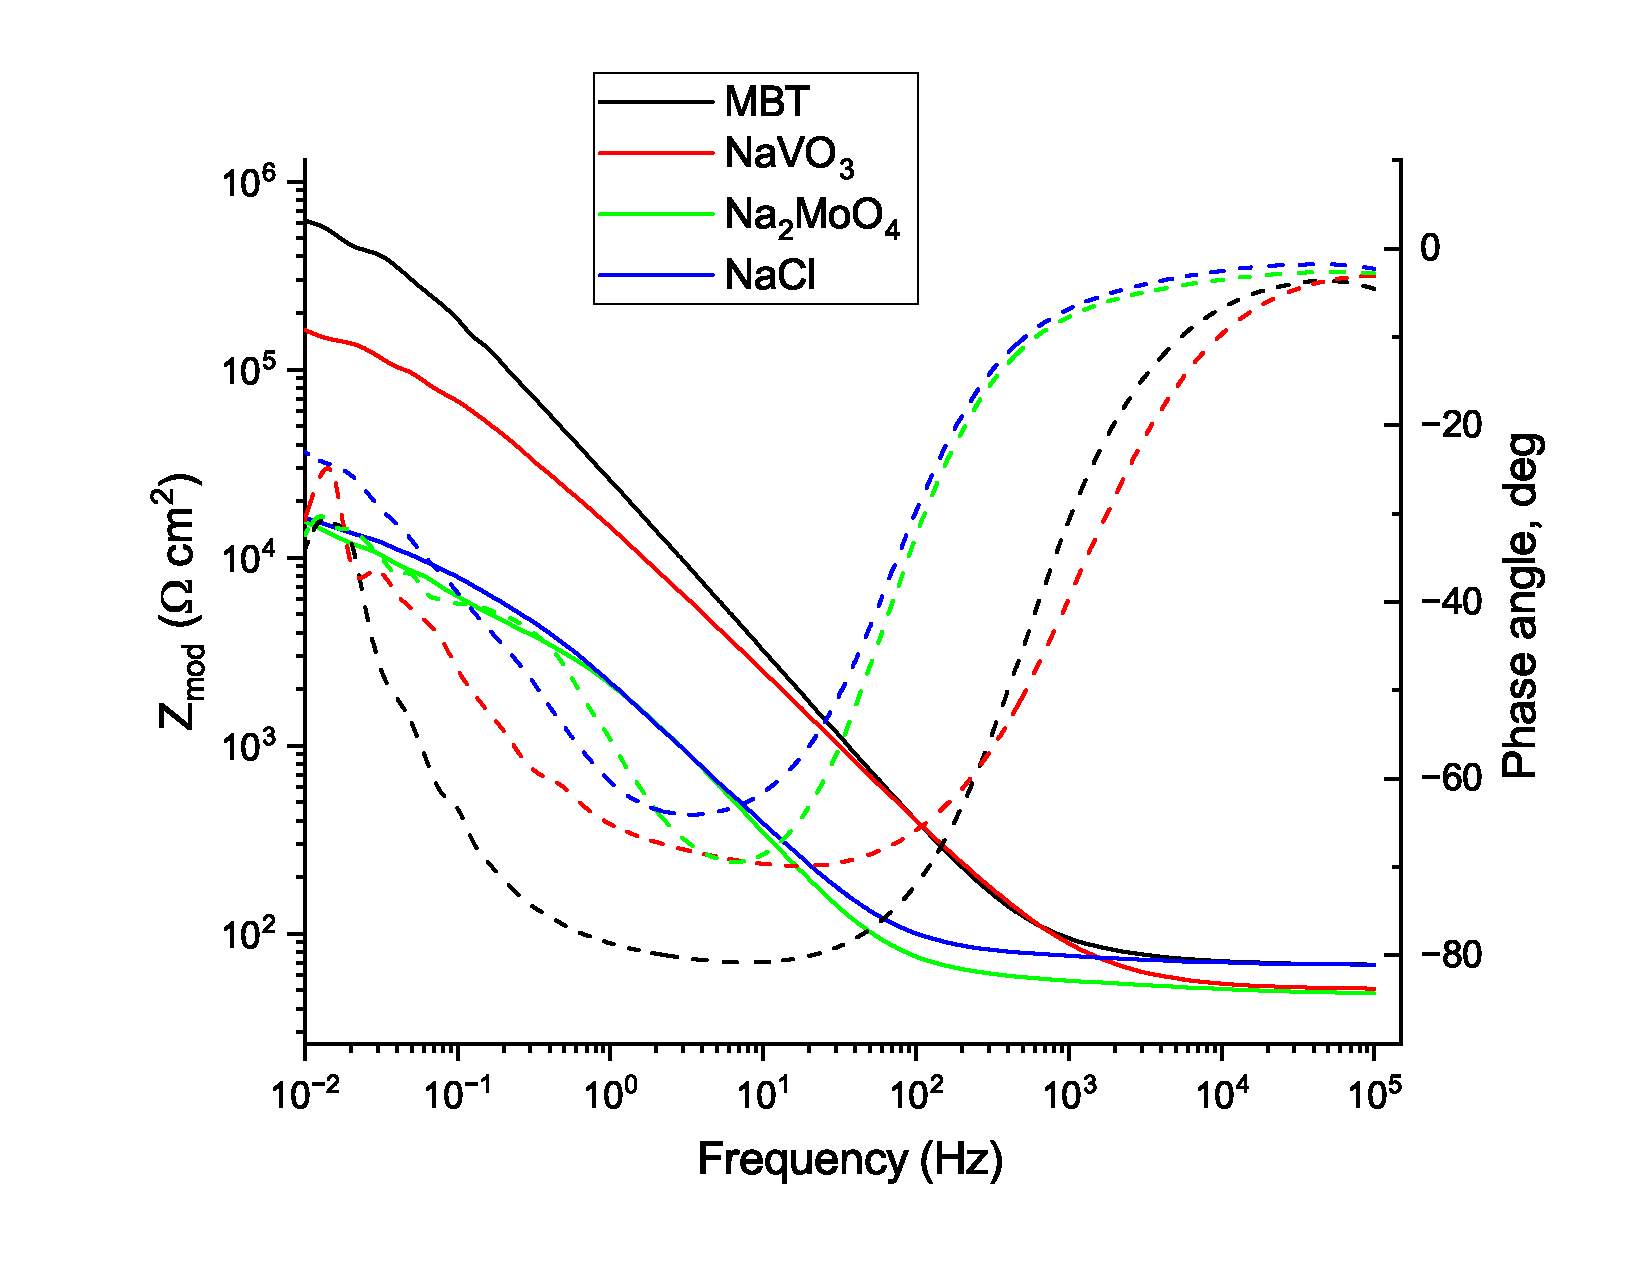
\includegraphics[width=\textwidth]{plots/Bode_8h.eps}
         \caption{}
         \label{fig:Bode8h}
     \end{subfigure}
     \hfill
     \begin{subfigure}[b]{0.48\textwidth}
         \centering
         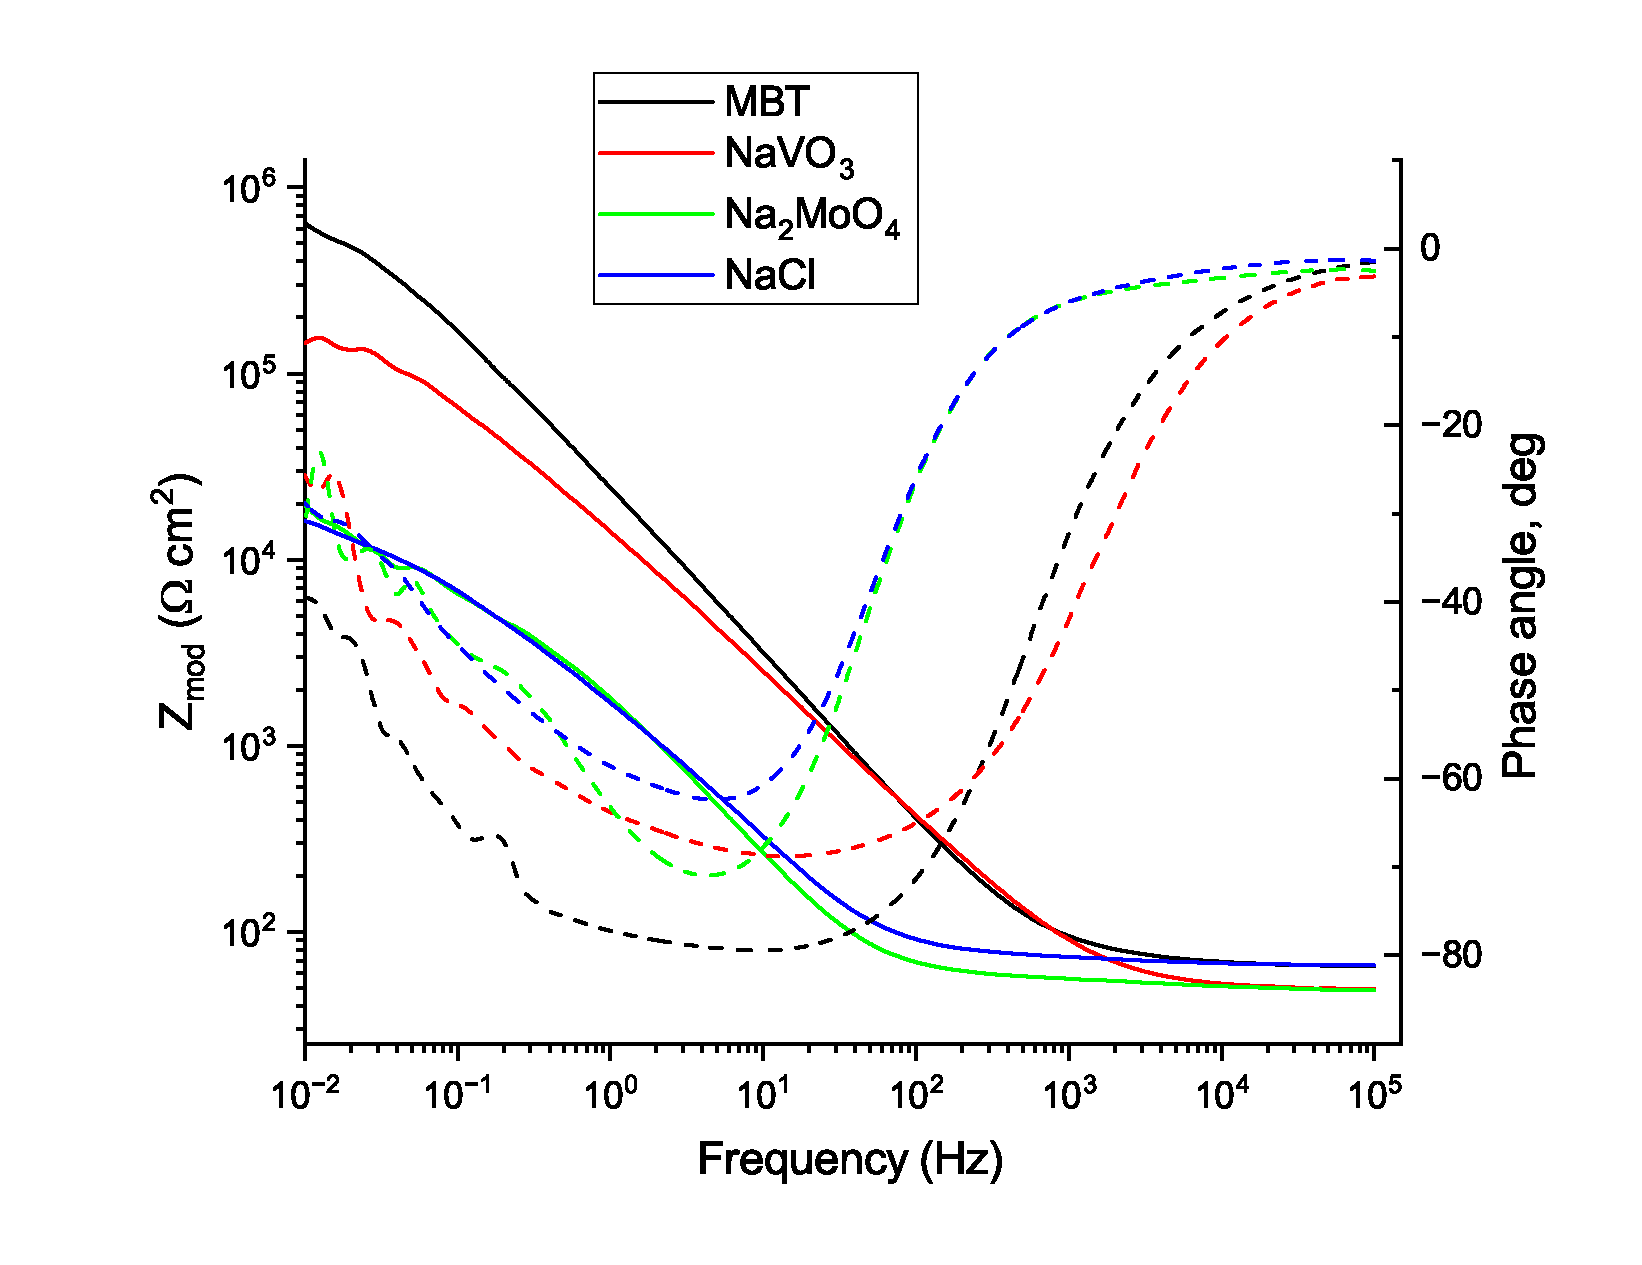
\includegraphics[width=\textwidth]{plots/Bode_24h.eps}
         \caption{}
         \label{fig:Bode24h}
     \end{subfigure}
     \caption{(a),(b),(c) and (d) Bode plots obtained for AC46000 after 1h, 4h, 8h, and 24h of immersion in 0.05 M NaCl with and without inhibitors.}
     \label{Bodeplots2}
\end{figure}

\begin{figure}[t]
     \ContinuedFloat
     \centering
     \begin{subfigure}[b]{0.48\textwidth}
         \centering
         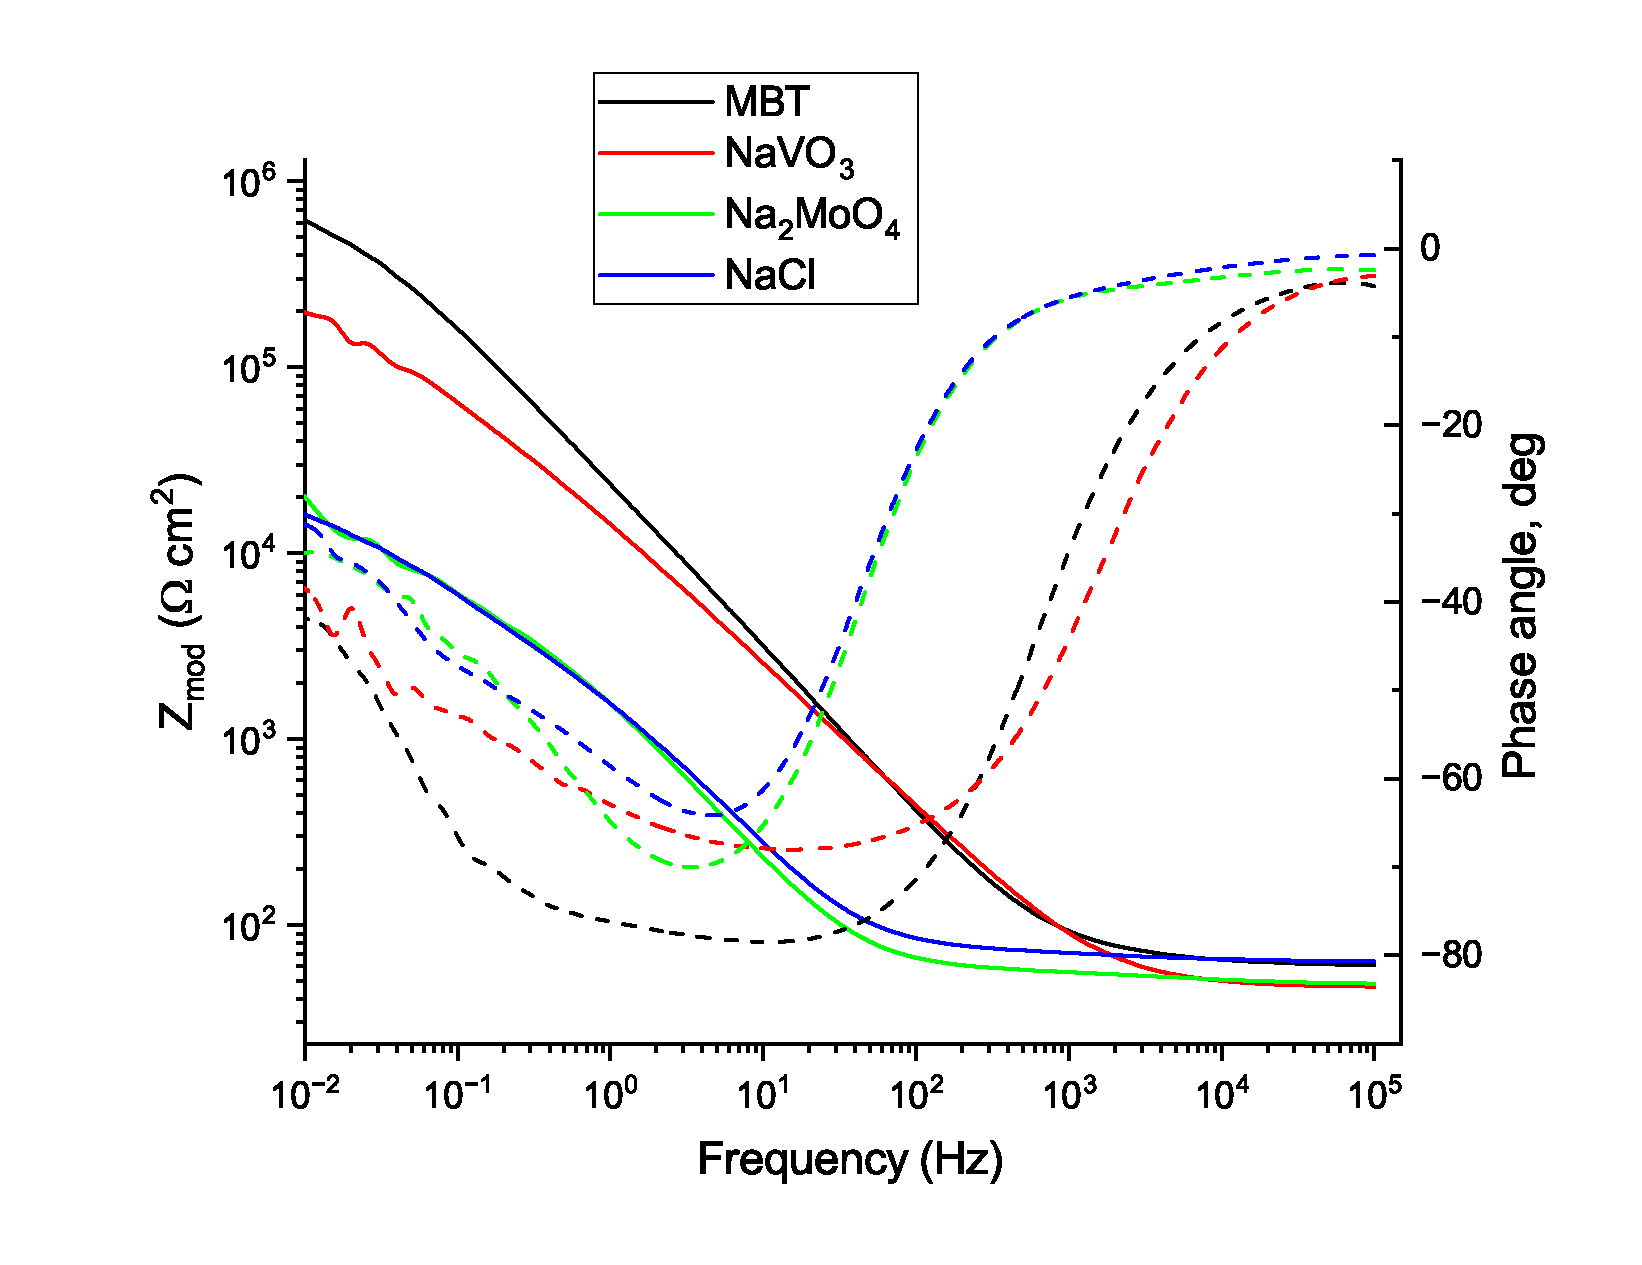
\includegraphics[width=\textwidth]{plots/Bode_48h.eps}
         \caption{}
         \label{fig:Bode48h}
     \end{subfigure}
     \hfill
     \begin{subfigure}[b]{0.48\textwidth}
         \centering
         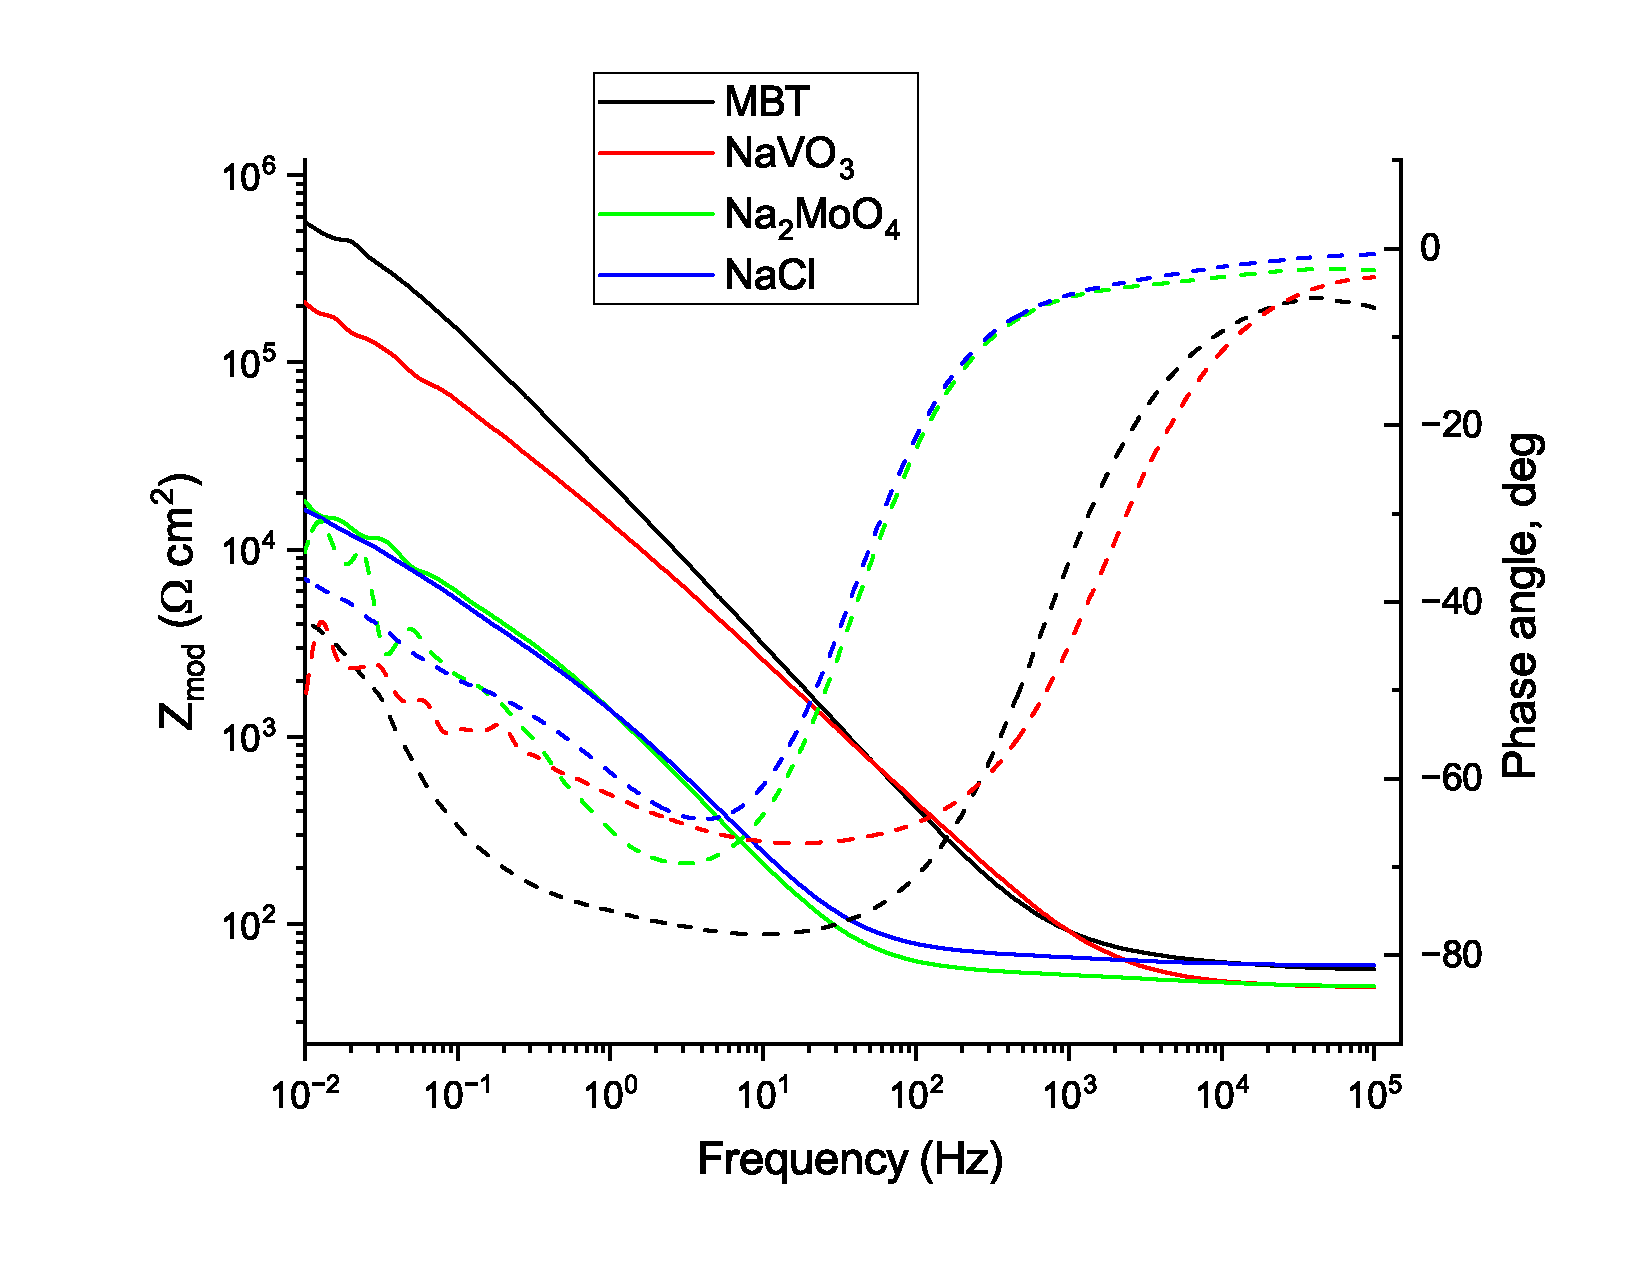
\includegraphics[width=\textwidth]{plots/Bode_72h.eps}
         \caption{}
         \label{fig:Bode72h}
     \end{subfigure}

     \vspace{0.5cm}

     \begin{subfigure}[b]{0.48\textwidth}
         \centering
         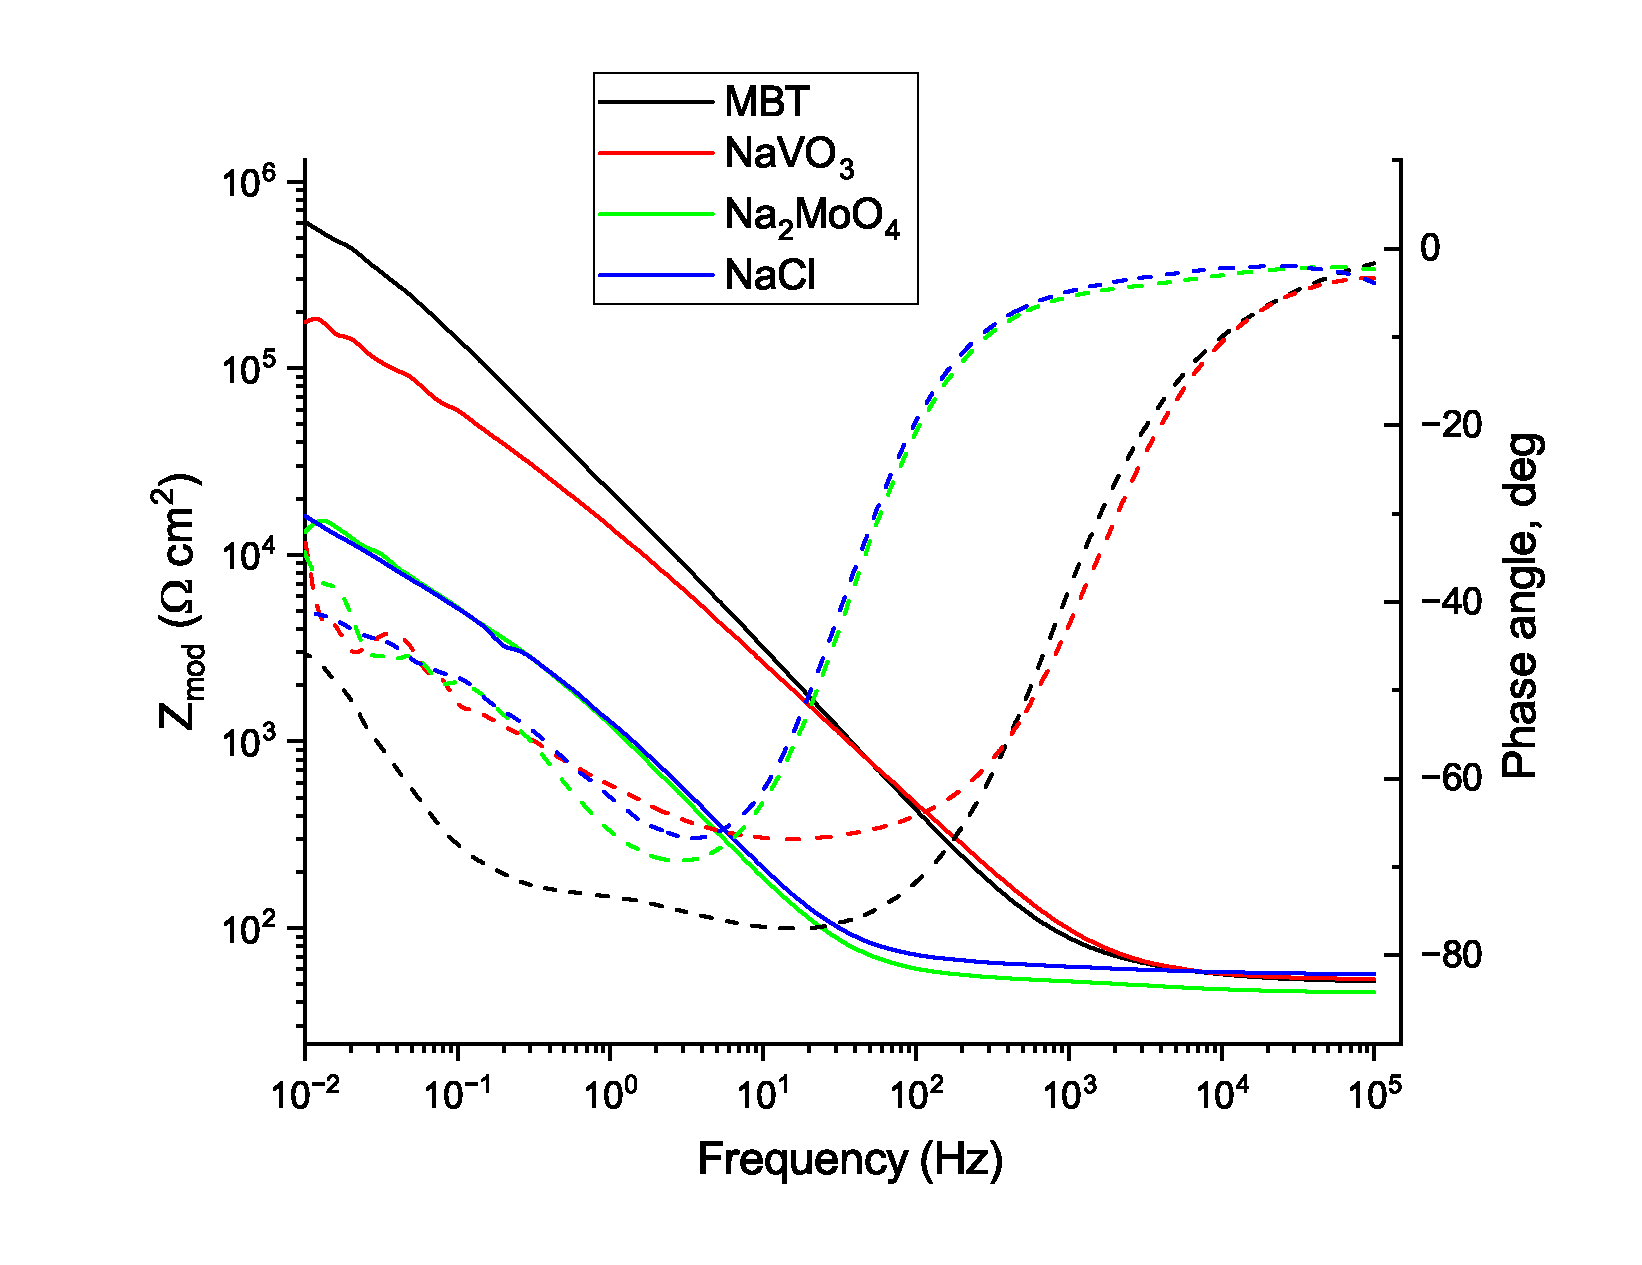
\includegraphics[width=\textwidth]{plots/Bode_120h.eps}
         \caption{}
         \label{fig:Bode120h}
     \end{subfigure}
     \hfill 
     \begin{subfigure}[b]{0.48\textwidth}
         \centering
         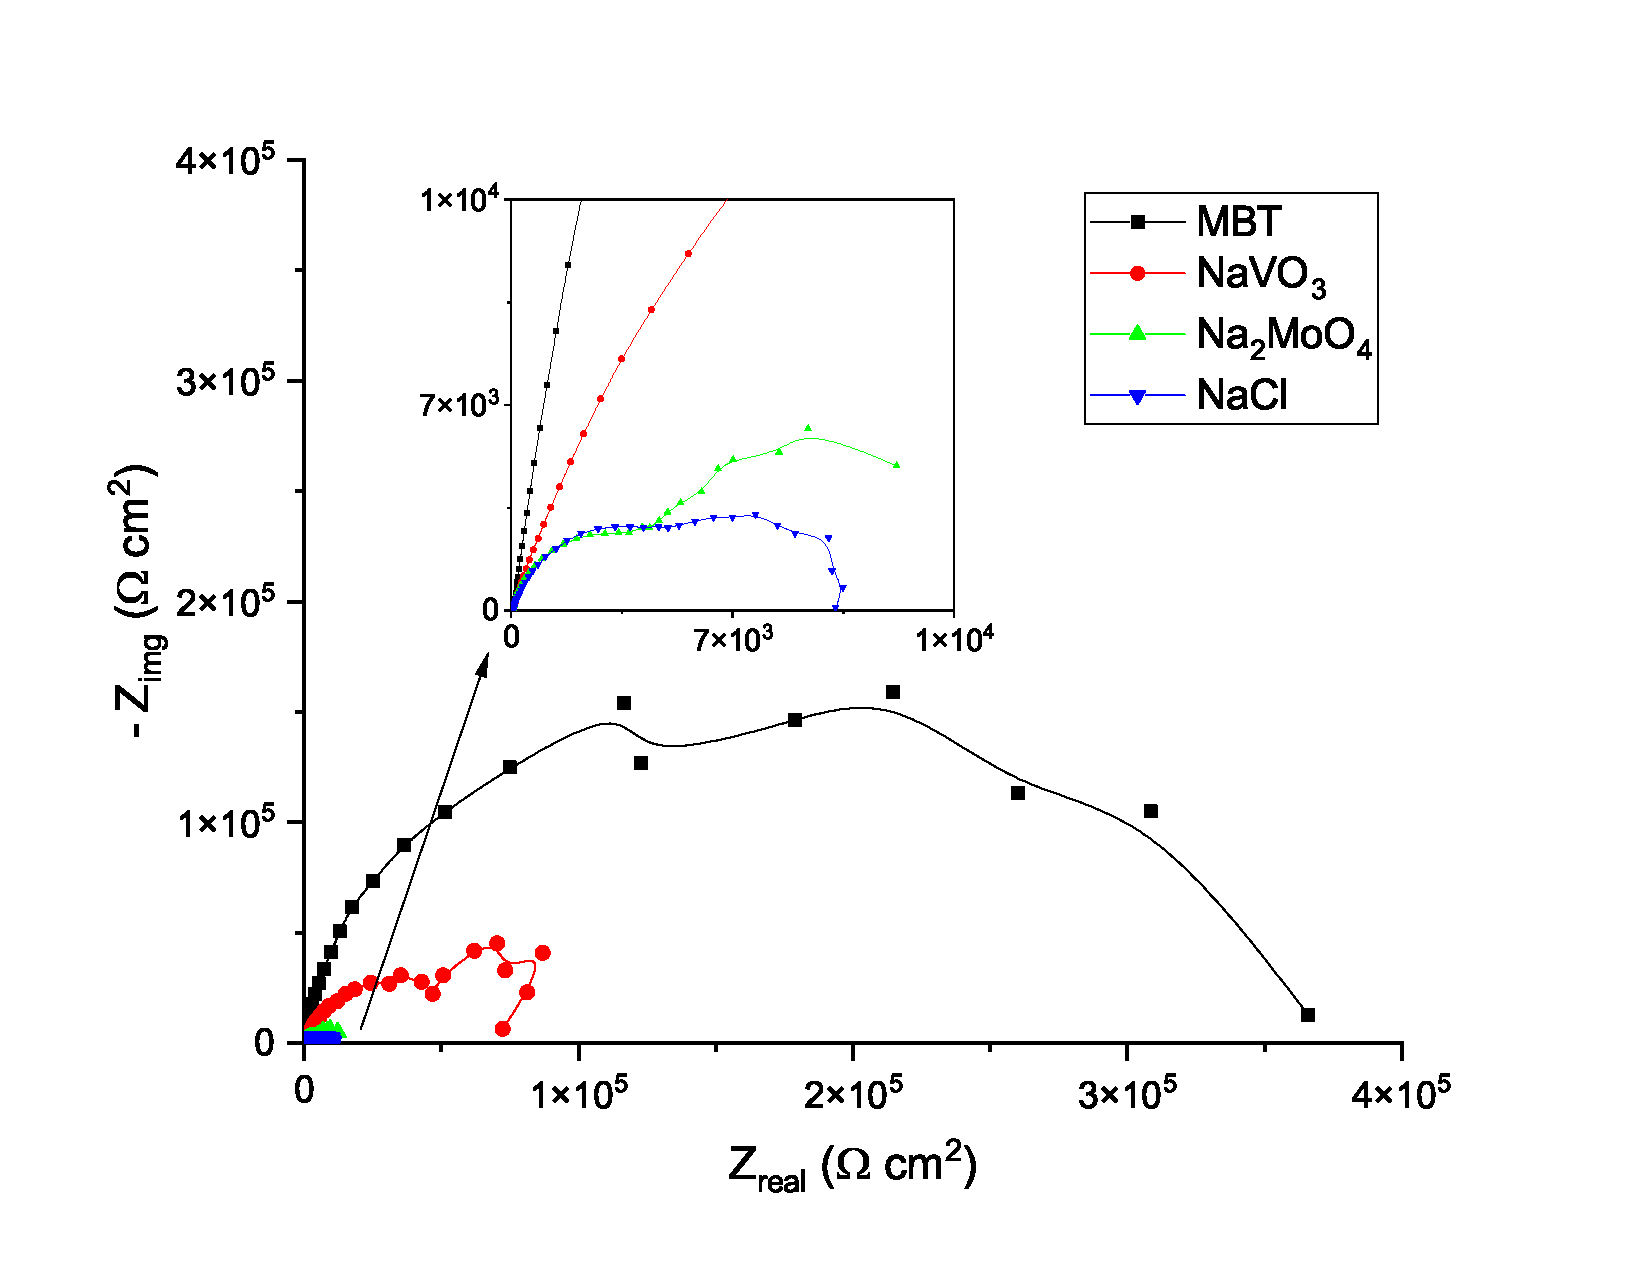
\includegraphics[width=\textwidth]{plots/Nyquist_1h_3.eps}
         \caption{}
         \label{fig:Nyquist1h}
     \end{subfigure}

     \vspace{0.5cm}

     \begin{subfigure}[b]{0.48\textwidth}
         \centering
         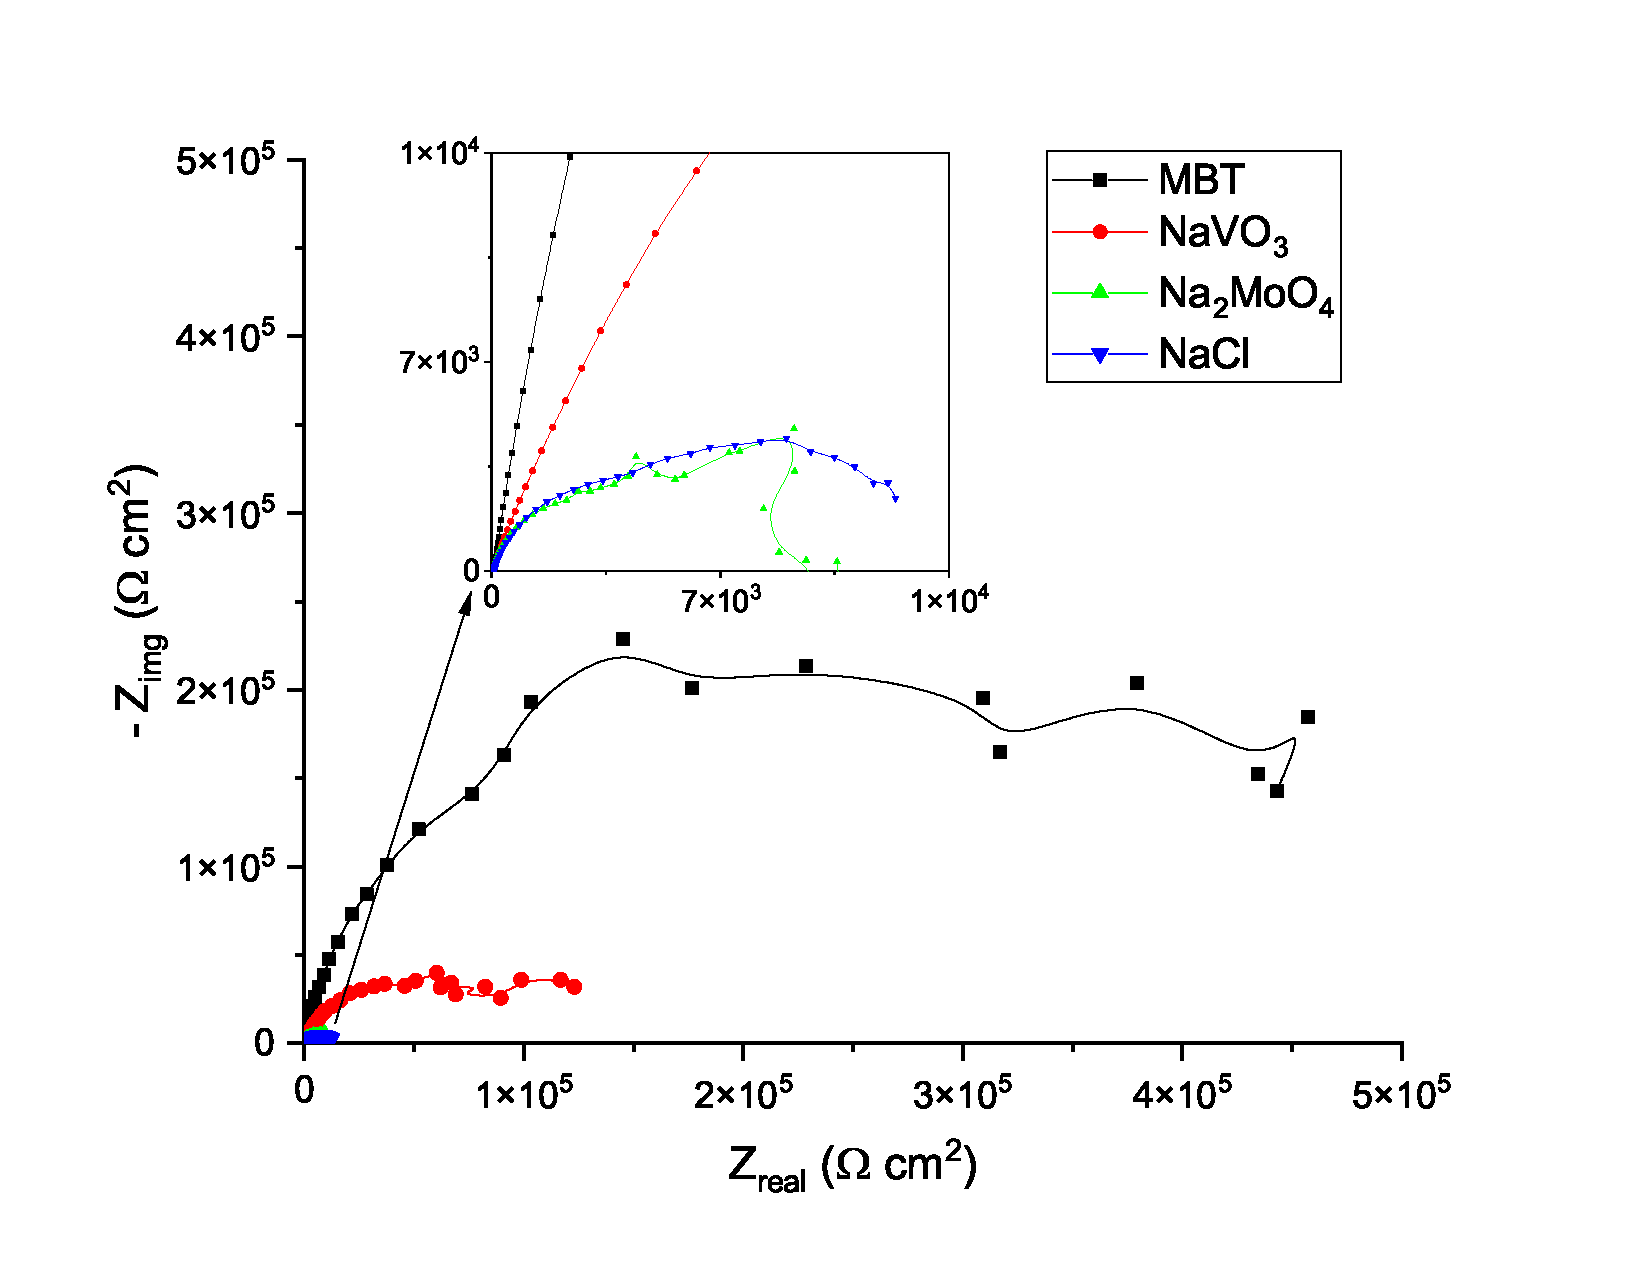
\includegraphics[width=\textwidth]{plots/Nyquist_4h_3.eps}
         \caption{}
         \label{fig:Nyquist4h}
     \end{subfigure}
     \hfill
     \begin{subfigure}[b]{0.48\textwidth}
         \centering
         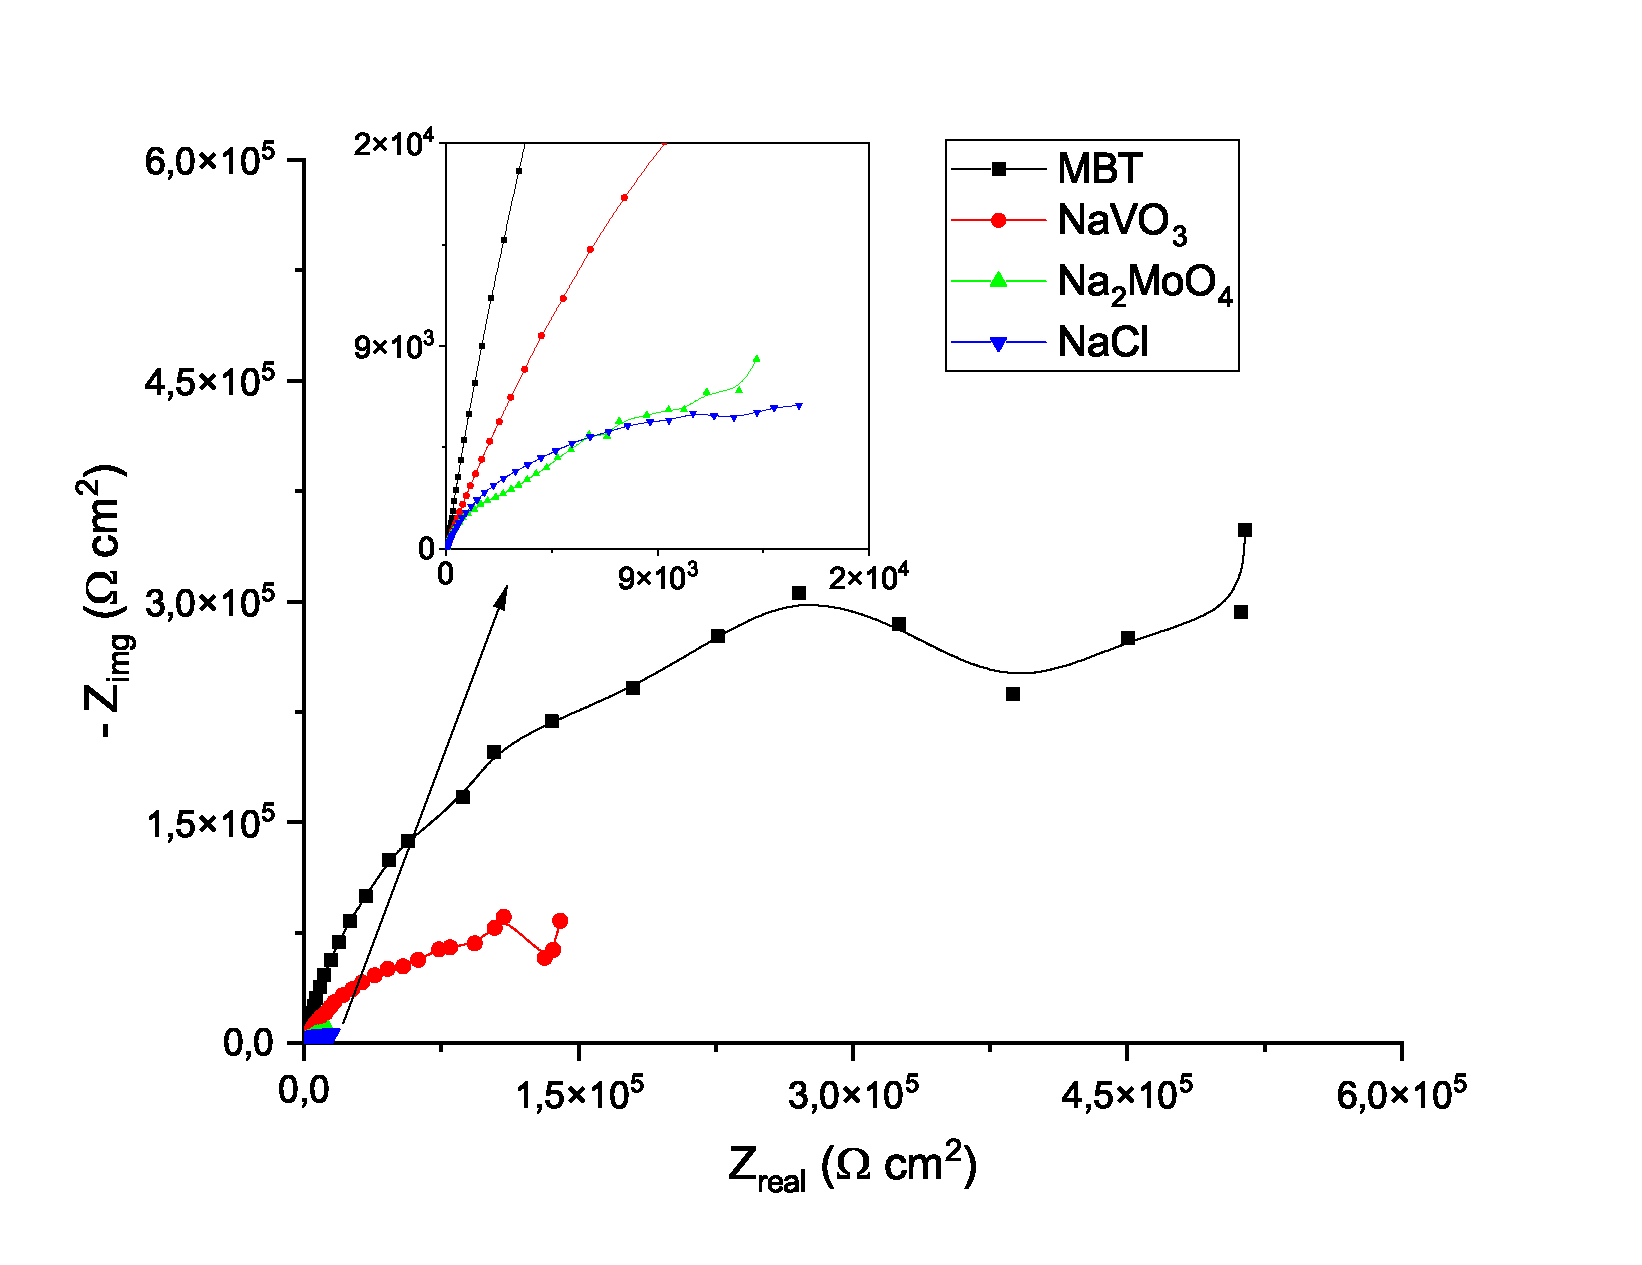
\includegraphics[width=\textwidth]{plots/Nyquist_8h_3.eps}
         \caption{}
         \label{fig:Nyquist8h}
     \end{subfigure}
     \caption{(e),(f) and (g) Bode plots obtained for AC46000 after 48h, 72h and 120h of immersion in 0.05 M NaCl with and without inhibitors; (h),(i) and (j) Nyquist plots obtained for AC46000 after 1h, 4h and 8h of immersion in 0.05 M NaCl with and without inhibitors;}
     \label{Nyquistplots1}
\end{figure}

\begin{figure}[!ht]
     \ContinuedFloat
     \centering
     \begin{subfigure}[b]{0.48\textwidth}
         \centering
         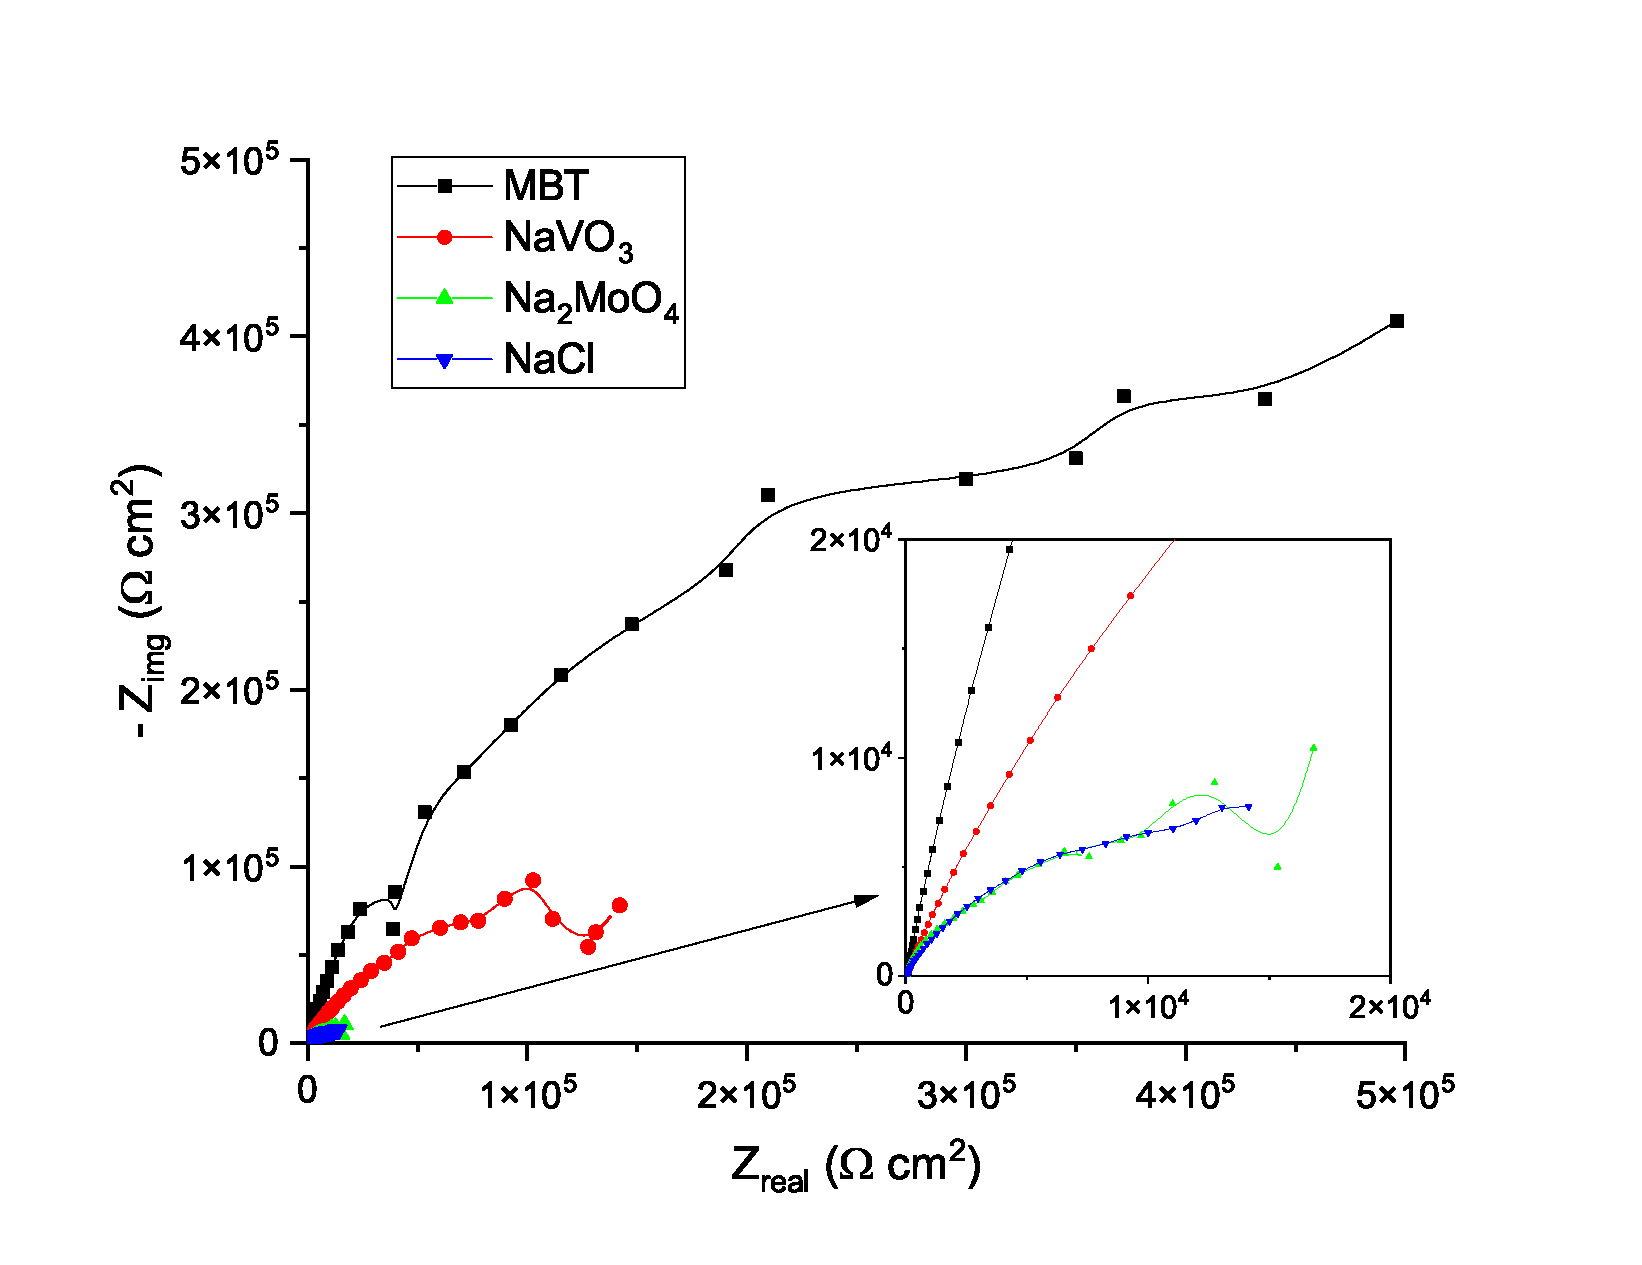
\includegraphics[width=\textwidth]{plots/Nyquist_24h_3.eps}
         \caption{}
         \label{fig:Nyquist24h}
     \end{subfigure} 
     \hfill
     \begin{subfigure}[b]{0.48\textwidth}
         \centering
         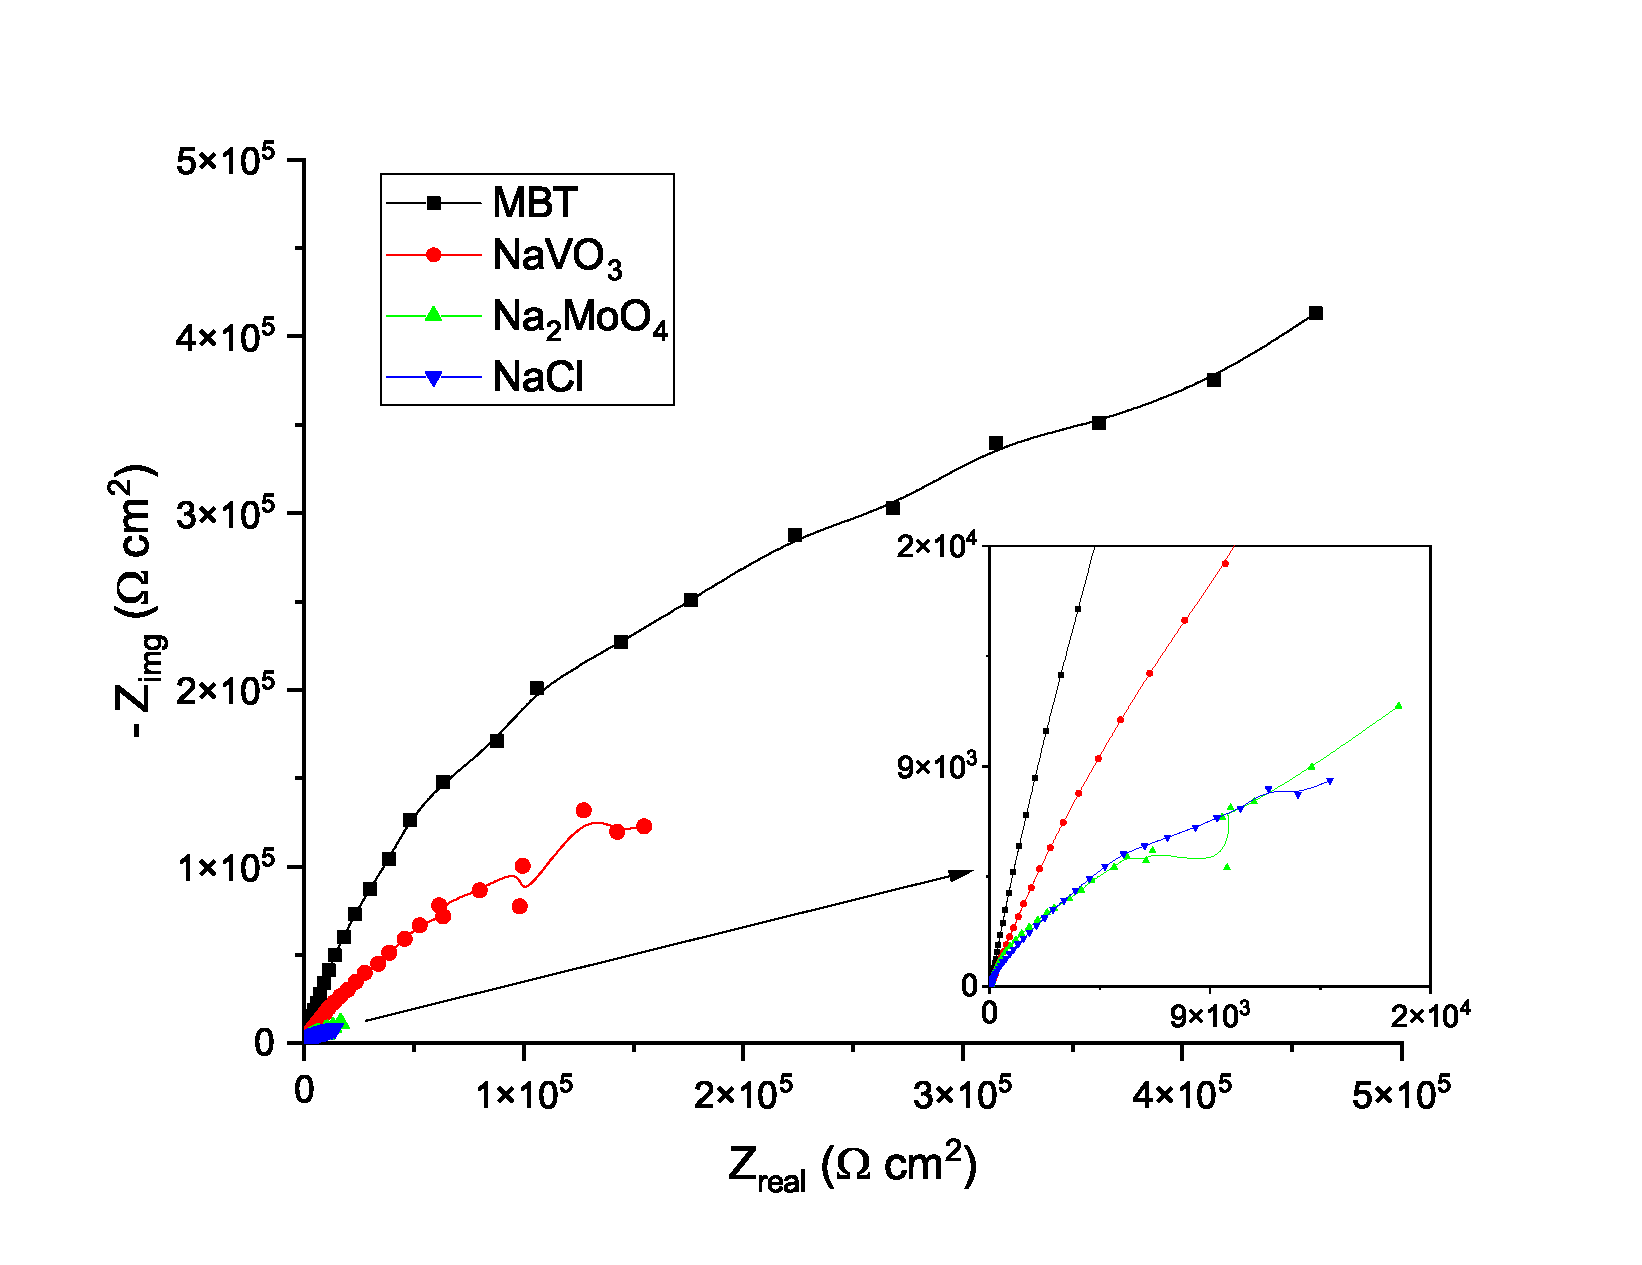
\includegraphics[width=\textwidth]{plots/Nyquist_48h_3.eps}
         \caption{}
         \label{fig:Nyquist48h}
     \end{subfigure}

     \vspace{0.5cm}

     \begin{subfigure}[b]{0.48\textwidth}
         \centering
         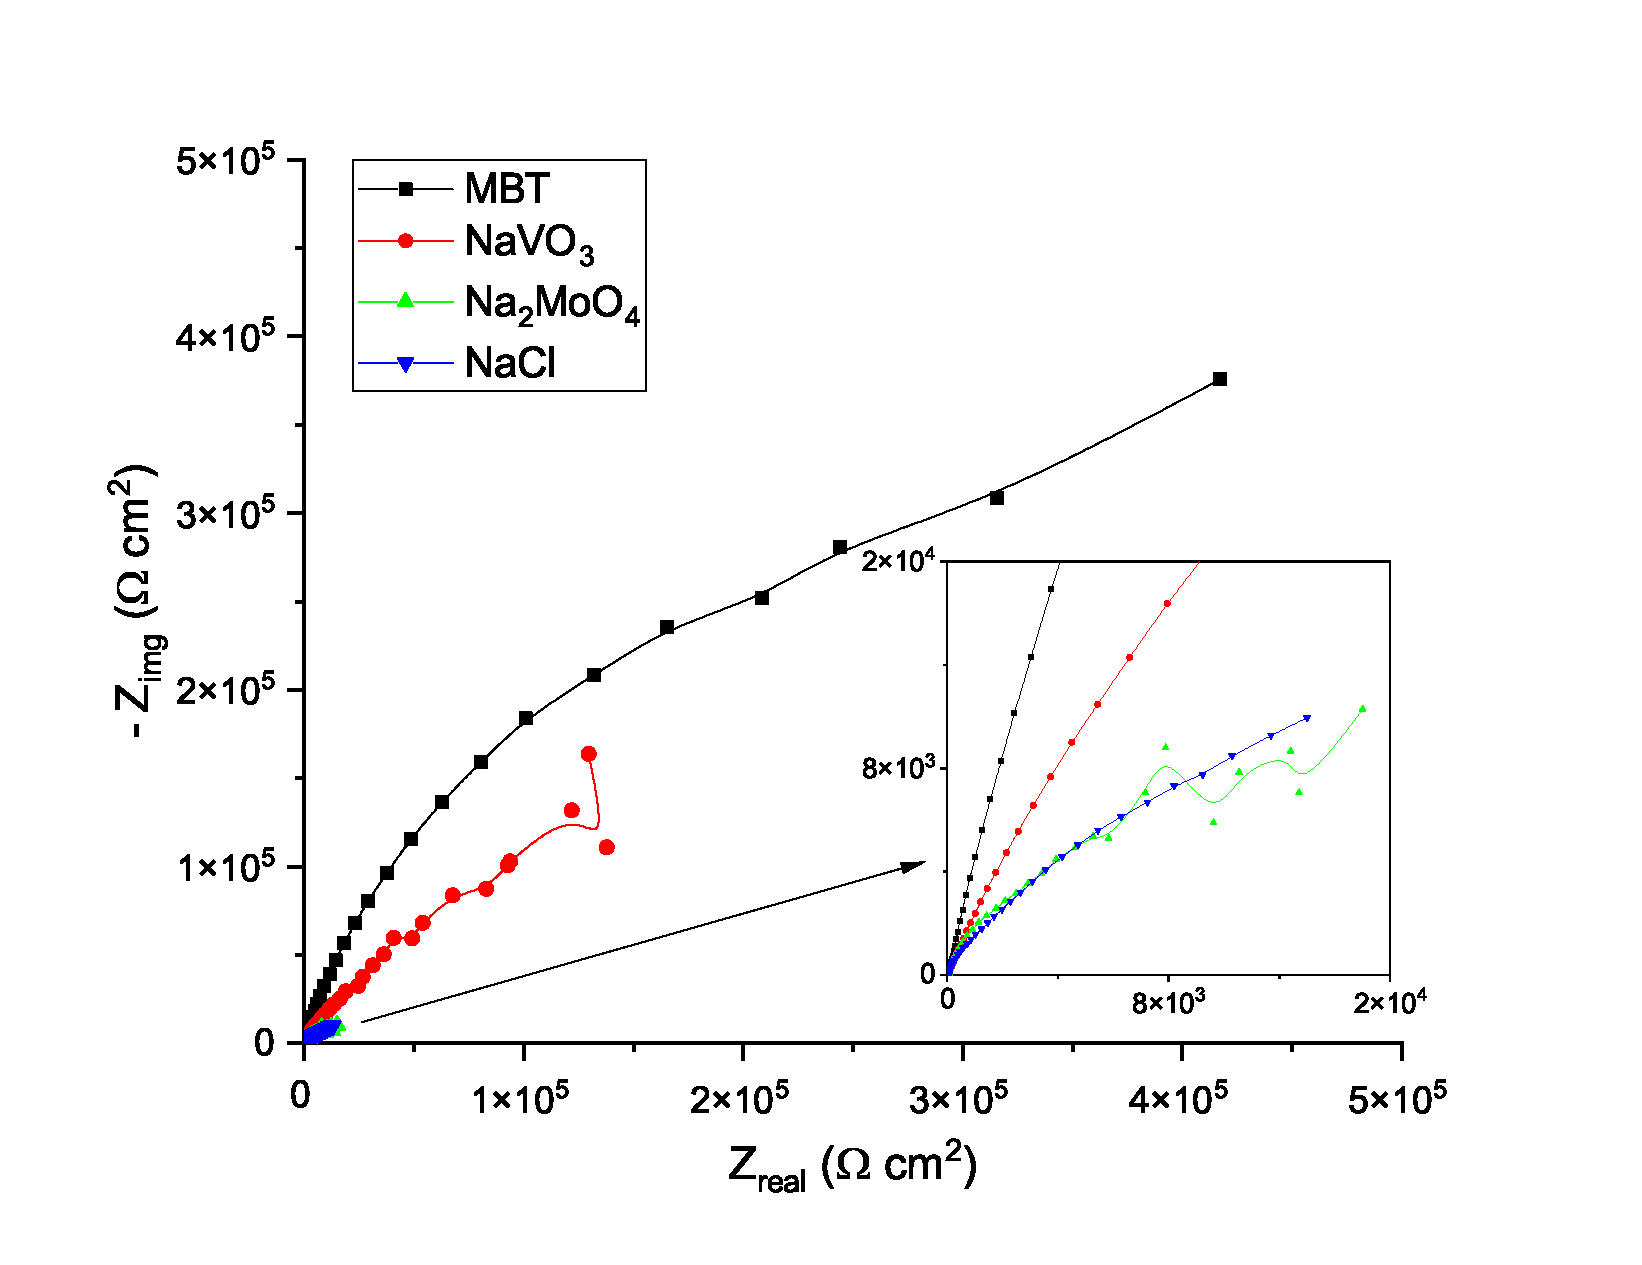
\includegraphics[width=\textwidth]{plots/Nyquist_72h_3.eps}
         \caption{}
         \label{fig:Nyquist72h}
     \end{subfigure}
     \hfill 
     \begin{subfigure}[b]{0.48\textwidth}
         \centering
         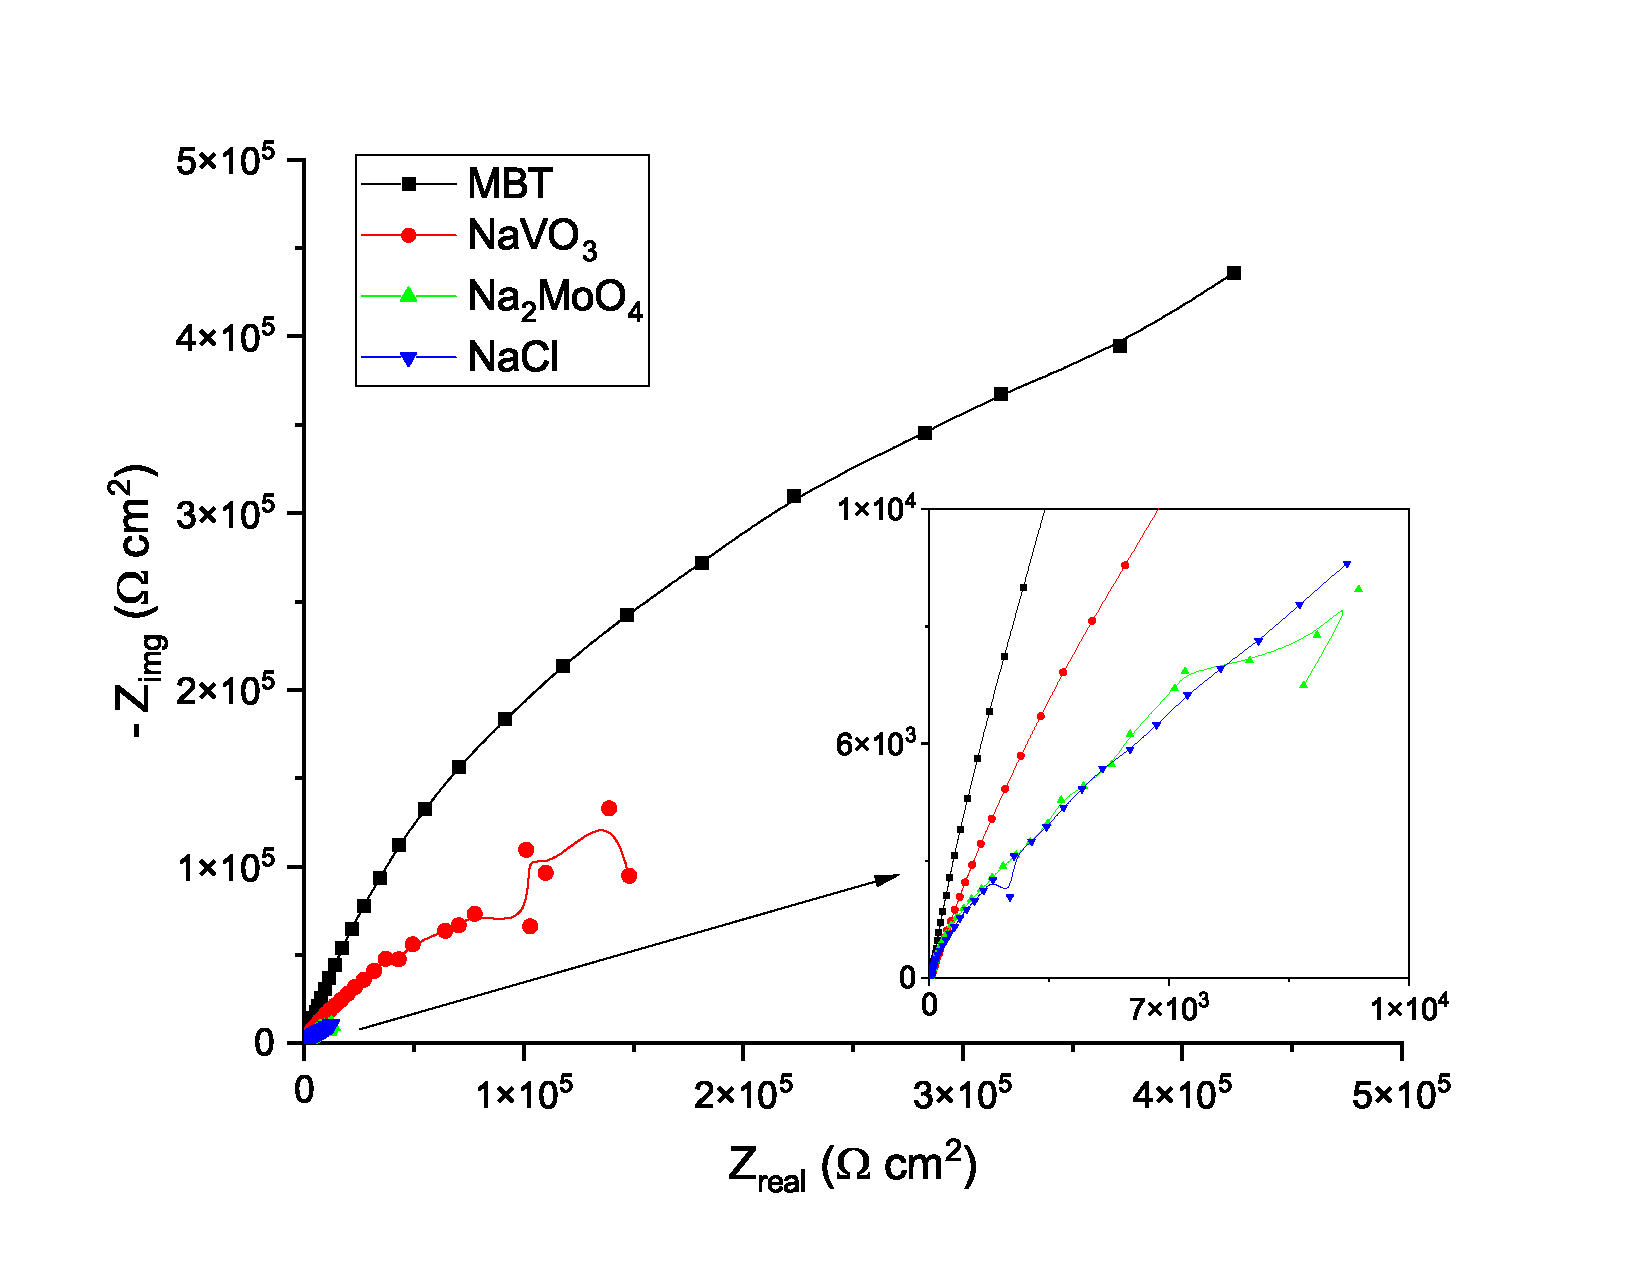
\includegraphics[width=\textwidth]{plots/Nyquist_120h_3.eps}
         \caption{}
         \label{fig:Nyquist120h}
     \end{subfigure}
     \caption{(k),(l),(m) and (n) Nyquist plots obtained for AC46000 after 24h, 48h, 72h and 120h of immersion in 0.05 M NaCl with and without inhibitors;} 
     \label{Nyquistplots2}
\end{figure}


\end{document}
